\documentclass[10pt, svgnames]{beamer}

\usetheme{Singapore}
%% \usetheme{Frankfurt}
%% \usecolortheme{seahorse}
% \usetheme{Madrid}
\setbeamertemplate{navigation symbols}{}
\setbeamertemplate{footline}[frame number]

\usepackage{etex}
\usepackage{xcolor}
\usepackage{ctable}
\usepackage{multirow}
\usepackage{tikz}
\usepackage{amsmath}
\usepackage{atlasphysics}
\usepackage{brett_latex_commands}
\usepackage[normalem]{ulem}
\usepackage{nicefrac}

% \setbeamerfont{block title}{size=\scriptsize}

% ------------------------------------------------------------------------------
%% \newcommand{\Stop}{\ensuremath{\tilde{t}}}
%% \newcommand{\AntiStop}{\ensuremath{\tilde{t}^{*}}}
%% \newcommand{\TTBAR}{\ensuremath{t\bar{t}}}
%% \newcommand{\ZGAMMA}{\ensuremath{Z/\gamma^{*}}}
%% \newcommand{\Ht}{\ensuremath{H_\mathrm{T}}}
%% \newcommand{\Met}{\ensuremath{E^\mathrm{miss}_\mathrm{T}}}
%% \newcommand{\MetRel}{\ensuremath{E^\mathrm{miss,rel}_\mathrm{T}}}
%% \newcommand{\MetSig}{\ensuremath{E^\mathrm{miss}_\mathrm{T}\mathrm{ significance}}}
%% \newcommand{\MetSigEqn}{\ensuremath{E^\mathrm{miss}_\mathrm{T}/\sqrt{\Ht}}}
%% \newcommand{\Mll}{\ensuremath{m_{\ell\ell}}}
%% \newcommand{\Mbl}{\ensuremath{m_{\mathrm{b}\ell}}}
%% \newcommand{\MblAsym}{\ensuremath{m_{\mathrm{b}\ell}\mathrm{~asymmetry}}}
%% \newcommand{\MblAsymEqn}{\ensuremath{\left(\Mbl^0-\Mbl^1\right)/\left(\Mbl^0+\Mbl^1\right)}}

% ------------------------------------------------------------------------------
\newcommand{\beginbackup}{
   \newcounter{framenumbervorappendix}
   \setcounter{framenumbervorappendix}{\value{framenumber}}
}
\newcommand{\backupend}{
   \addtocounter{framenumbervorappendix}{-\value{framenumber}}
   \addtocounter{framenumber}{\value{framenumbervorappendix}} 
}

% ------------------------------------------------------------------------------
\title{
  A search for \BMINUSL\ $R$-Parity violating scalar top decays
  % in $\sqrt{s} = 8~\TeV$ pp collisions with the ATLAS experiment
}
% \subtitle{PhD Thesis Defense}
\author[Brett Jackson]{
  \textcolor{blue}{Brett Jackson}
  \\
  Evelyn Thomson
}
% \institute{University of Pennsylvania}


\begin{document}

% ------------------------------------------------------------------------------
\begin{frame}
  \titlepage
  \centering{
    \begin{columns}
      \column{0.25\textwidth}
      \hfill
        
\includegraphics[height=0.25\textheight]{shield.pdf}
      \column{0.50\textwidth}
      \centering{
        {\color{red} PhD Thesis Defense}
      }
      \column{0.25\textwidth}
        
\includegraphics[height=0.25\textheight]{ATLAS_White_560x720_01.jpg}
    \end{columns}
  }
\end{frame}

% ==============================================================================
\section{Introduction}

% ------------------------------------------------------------------------------
\begin{frame}
  \frametitle{About me}
  \begin{columns}
    \column{0.6\linewidth}
    \begin{description}[0ex]
      \item[2008-2010] (Philadelphia) \\
        \begin{itemize}
          \item Classes at Penn
          \item TRT timing studies
        \end{itemize}
      \item[2010-2012] (\cern) \\
        \begin{itemize}
          \item Continued work on TRT
          \item Muon isolation
          \item Small studies for $Z'$ search
        \end{itemize}
      \item[2012-2013] (\cern) \\
        \begin{itemize}
          \item Started working in SUSY group
          \item Search for direct gaugino production
        \end{itemize}
      \item[2013-2015] (\cern) \\
        \begin{itemize}
          \item \BMINUSL\ stop search (This talk)
        \end{itemize}
    \end{description}
    %%
    \column{0.4\linewidth}
    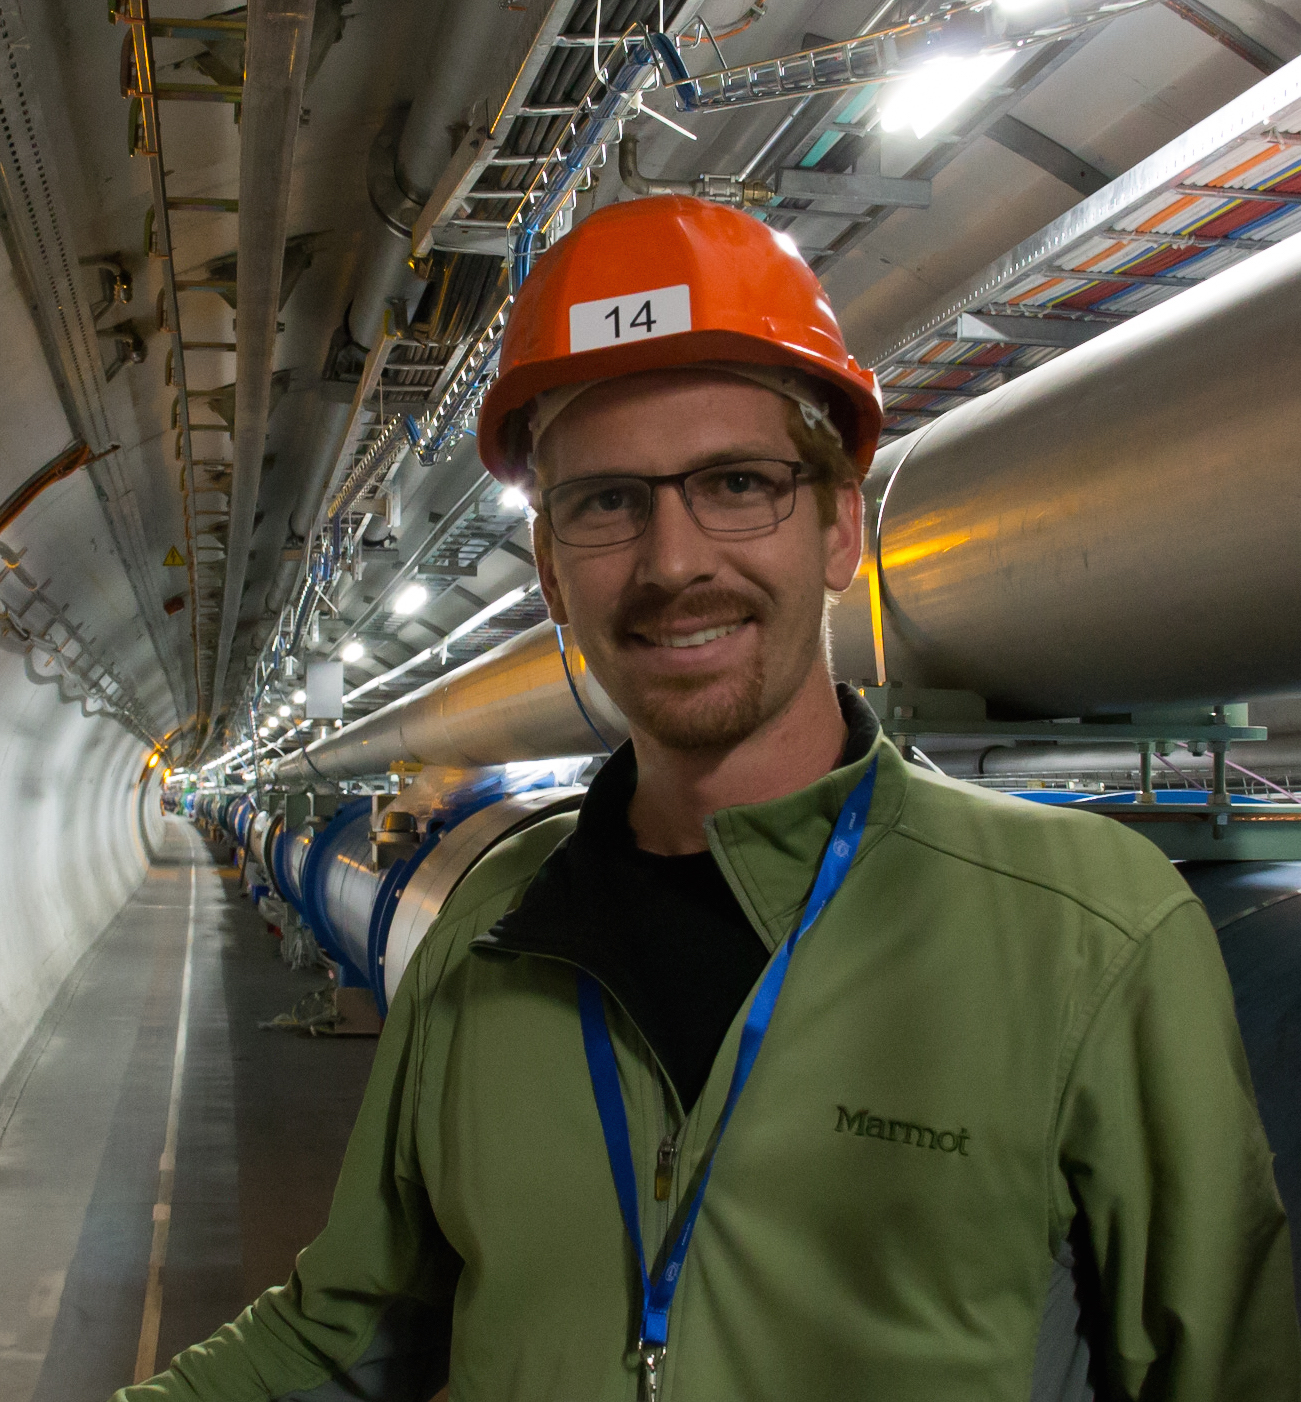
\includegraphics[
      width=\textwidth
    ]
    {figures/IMG_5092.jpg}
  \end{columns}
\end{frame}

% ------------------------------------------------------------------------------
% Display TOC and set up so that TOC is displayed before each section
\begin{frame}{Table of contents}
  \tableofcontents
\end{frame}

\AtBeginSection[]
{
  \begin{frame}{Table of contents}
    \tableofcontents[currentsection]
  \end{frame}
}

% ==============================================================================
\section{Theoretical motivation}
\subsection{Standard Model}

% ------------------------------------------------------------------------------
\begin{frame}
  \frametitle{Standard Model}
  %%
  \begin{itemize}
    \item Quantum field theory
    \item Describes matter and electroweak and strong interactions
    \item Tested over the last \textbf{50 years}!
  \end{itemize}
  %%
  \begin{center}
    \begin{tikzpicture}
      \node[
        anchor=south west,
        inner sep=0
      ] (image) at (0,0) {
        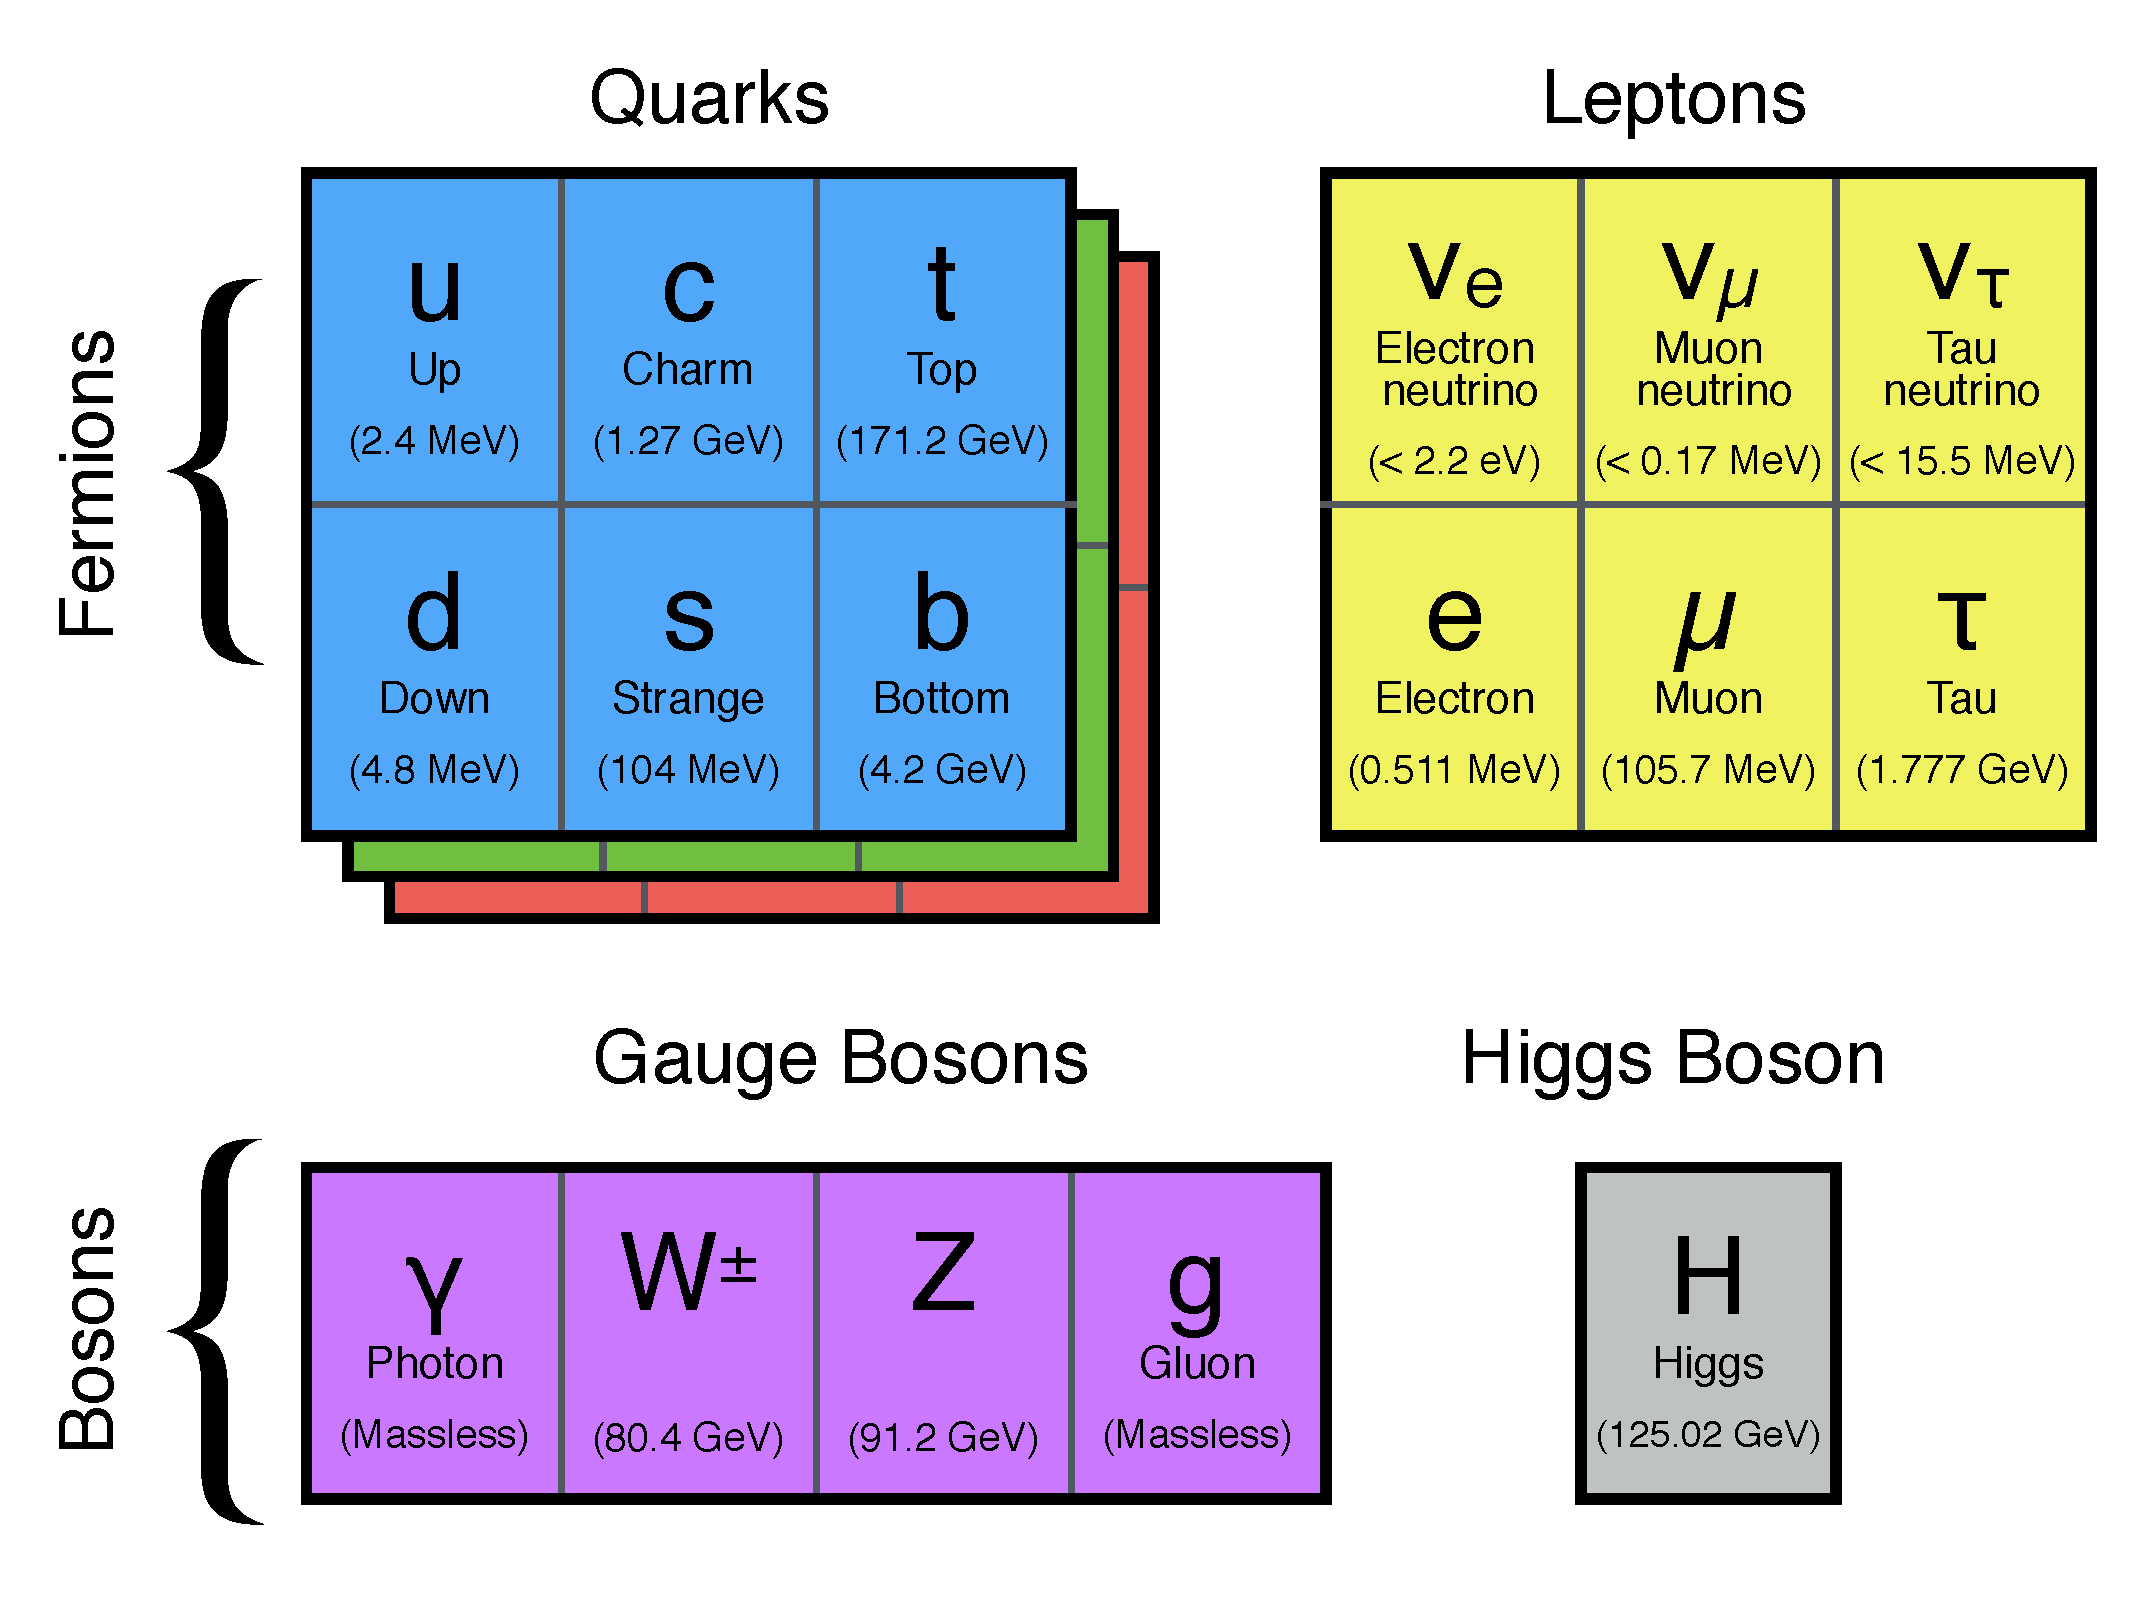
\includegraphics[width=0.65\textwidth]
        {figures/theory/sm_particle_content.pdf}
      };
      \begin{scope}[
          x={(image.south east)}, y={(image.north west)}
        ]
        %%
        \draw[
          nice_red,
          ultra thick,
          rounded corners
        ]
        (0.67, 0.02)
        rectangle
        (0.90, 0.40);
        %%
        \node[
          rectangle,
          rounded corners=1ex,
          fill=nice_blue,
          text=white,
          anchor=west
        ]
        at (0.95, 0.25) {
          \footnotesize
          \begin{tabular}{c}
            Missing until \\ 2012!
          \end{tabular}
        };
        %%
        %% \MyGrid
      \end{scope}
    \end{tikzpicture}
  \end{center}
\end{frame}

% ------------------------------------------------------------------------------
\begin{frame}
  \frametitle{Higgs boson discovery!}
  %%
  \begin{itemize}
    \item July 4, 2012: Announced discovery of a ``new boson''
    \item Scalar particle with mass of 125~\GeV
    \item Discovered in $\gamma\gamma$, $ZZ^{*}$, and $WW^{*}$ channels
    \item This turned out to be the Higgs boson
  \end{itemize}
  %%
  \vspace{1ex}
  %%
  \begin{columns}
    \column{0.45\textwidth}
    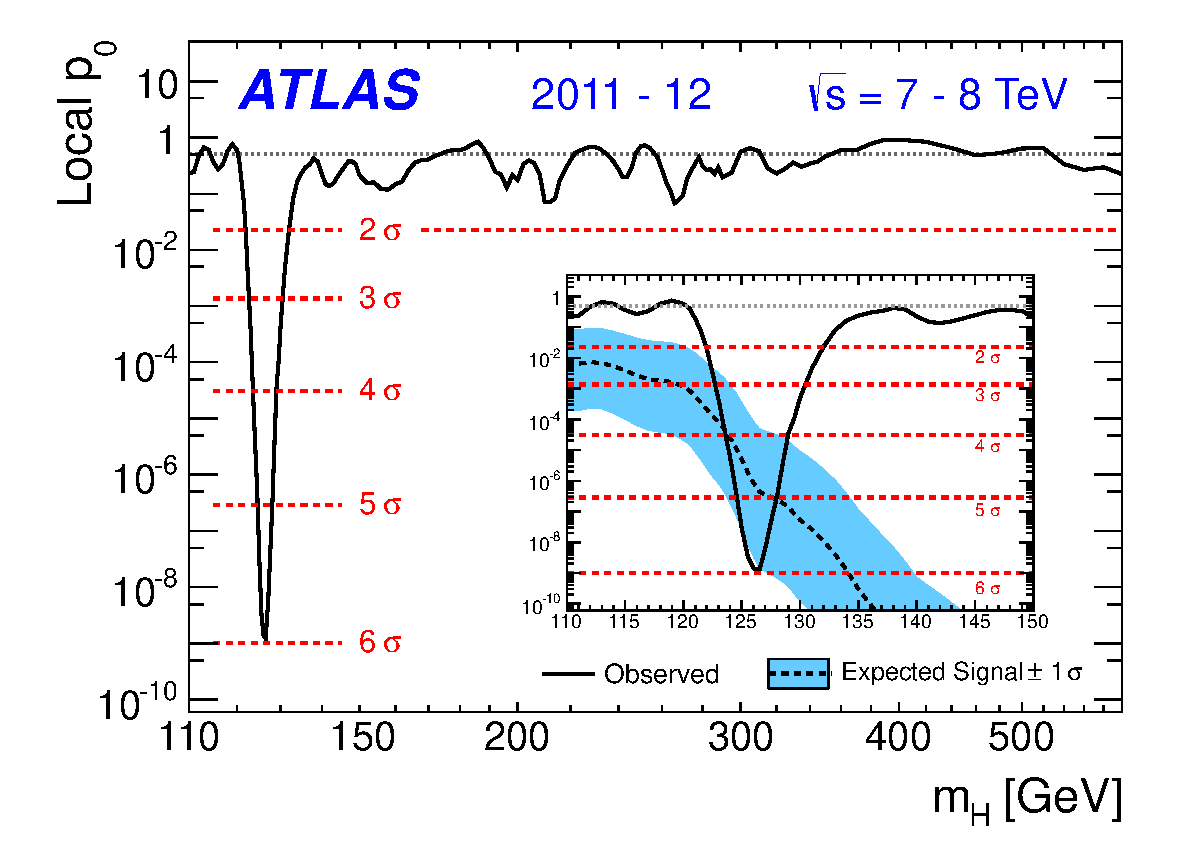
\includegraphics[width=\textwidth]{figures/theory/figaux_109.pdf}
    \column{0.55\textwidth}
    \begin{tikzpicture}
      \node[
        anchor=south west,
        inner sep=0,
      ] (image) at (0,0) {
        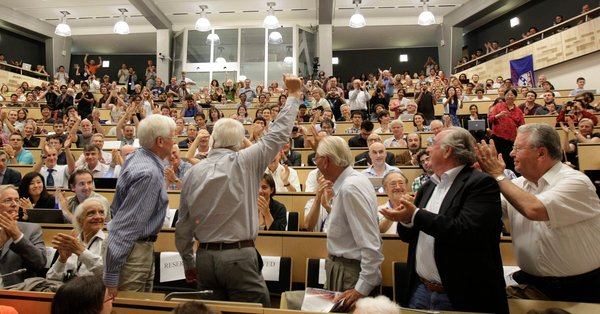
\includegraphics[width=\textwidth]{figures/theory/Higgs-articleLarge.jpg}
      };
      \begin{scope}[
          x={(image.south east)}, y={(image.north west)}
        ]
        %%
        % \draw[
        %   % -triangle 60,
        %   -stealth,
        %   nice_blue,
        %   ultra thick,
        %   % rounded corners
        % ]
        % (0.7, 0.90) -- (0.83, 0.80);
        %%
        \draw[
          nice_blue,
          ultra thick,
          rounded corners
        ]
        (0.75, 0.65) rectangle (0.95, 0.90);
        %%
        % \MyGrid
      \end{scope}
    \end{tikzpicture}
  \end{columns}
  %% \vspace{1ex}
  %% That's it, we can all go home...
\end{frame}

% ------------------------------------------------------------------------------
\begin{frame}
  \frametitle{Shortcomings}
  %%
  \begin{columns}
    \column{0.75\textwidth}
    \begin{itemize}
      % \item \sout{Gravity not included}
      \item Gravity not included
      % \item No neutrino masses, even with  BEH mechanism
      \item Missing dark matter candidate
      \item Hierarchy problem
        \begin{itemize}
          \item Large difference between electroweak scale and Planck scale
          \item Radiative corrections to Higgs mass diverge quadratically
          % \item Physical Higgs mass is difference between bare mass and
          %   radiative corrections
          \item Requires ``\textbf{\color{nice_blue} fine tuning}'' to obtain
            % physical Higgs mass of
            125~\GeV
        \end{itemize}
    \end{itemize}
    %%
    \column{0.25\textwidth}
    \begin{tikzpicture}[scale=0.9]
      \node[void] (in) at (0,0)  {};
      \node[void] (v1) at (1,0) {};
      \node[void] (v2) at (2,0) {};
      \node[void] (out) at (3,0) {};
      \draw[spin0] (in) -- node [above]{$H$} (v1) ;
      \draw (1.5,0) circle (0.5);
      \node at (1.5,0.7) {$f$};
      \draw[spin0] (v2) -- node [above]{$H$} (out);
    \end{tikzpicture}
    %%
    \vspace{0.75ex}
    %%
    \begin{tikzpicture}[scale=0.9]
      \node[void] (in) at (0,0)  {};
      \node[void] (v1) at (1,0) {};
      \node[void] (v2) at (2,0) {};
      \node[void] (out) at (3,0) {};
      \draw[massvect] (v1) arc(180:0:0.5) ;
      \node at (1.5,0.8) {$W,Z$};
      \draw[spin0] (in) -- node [above]{$H$} (v1) -- (v2) -- node [above]{$H$} (out);
    \end{tikzpicture}
    %%
    \vspace{0.75ex}
    %%
    \begin{tikzpicture}[scale=0.9]
      \node[void] (in) at (0,0)  {};
      \node[void] (v1) at (1,0) {};
      \node[void] (v2) at (2,0) {};
      \node[void] (out) at (3,0) {};
      \draw[massvect] (1.5,0.45) circle (0.5);
      \node at (1.5,1.3) {$W,Z$};
      \draw[spin0] (in) -- node [above]{$H$} (v1) -- (v2) -- node [above]{$H$} (out);
    \end{tikzpicture}
    %%
    \vspace{0.75ex}
    %%
    \begin{tikzpicture}[scale=0.9]
      \node[void] (in) at (0,0)  {};
      \node[void] (v1) at (1,0) {};
      \node[void] (v2) at (2,0) {};
      \node[void] (out) at (3,0) {};
      \draw[spin0] (1.5,0.5) circle (0.5);
      \node at (1.5,1.3) {$H$};
      %%
      \draw[spin0]
      (in) -- node [above]{$H$} (v1) -- (v2) -- node [above]{$H$} (out);
    \end{tikzpicture}
  \end{columns}
\end{frame}

% ==============================================================================
\subsection{Supersymmetry}

% ------------------------------------------------------------------------------
\begin{frame}
  \frametitle{Supersymmetry}
  %%
  \begin{itemize}
    \item Fermions and bosons have radiative corrections with opposite sign
    \item \textbf{\color{nice_blue} Double particle content} by introducing
      ``superpartners''
      \begin{itemize}
        \item SM fermions $\rightarrow$ boson ``sfermion''
        \item SM gauge bosons $\rightarrow$ fermion ``gaugino''
        \item Higgs doublet $\rightarrow$ Two Higgs supermultiplets +
          fermion ``Higgsinos''
      \end{itemize}
    \item Superpartners expected to have same mass as SM counterparts
    \item SUSY must be \textbf{\color{nice_blue} broken symmetry}!
  \end{itemize}
  %%
  \begin{center}
    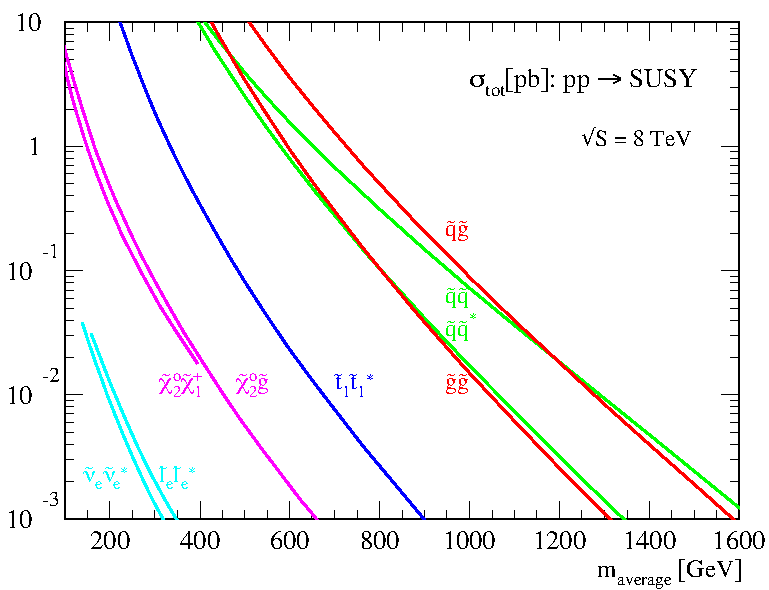
\includegraphics[width=0.5\textwidth]{figures/theory/prospino_lhc8.pdf}
  \end{center}
\end{frame}

% ------------------------------------------------------------------------------
\begin{frame}
  \frametitle{$R$-Parity}
  %%
  \begin{columns}
    %%
    \column{0.70\textwidth}
    \begin{itemize}
      \item Generic MSSM violates leptons and baryon number
        \begin{itemize}
          \item 
            $W_{\Delta L = 1} =
            \frac{1}{2} \lambda^{ijk} L_{i} L_{j} \bar{e}_{k} +
            \lambda'^{ijk} L_{i} Q_{j} \bar{d}_{k} +
            \mu'^{i} L_{i} H_\mathrm{u}$
          \item 
            $W_{\Delta B = 1} =
            \frac{1}{2} \lambda''^{ijk} \bar{u}_{i} \bar{d}_{j} \bar{d}_{k}$
        \end{itemize}
      \item Lead to proton decay!
      \item Forbid these by imposing {\color{nice_blue} $R$-Parity}
        conservation: $R=(-1)^{3(B-L)+2s}$
      \item SUSY particles cannot decay into (only) SM particle
      \item Can pair produce SUSY particles, but need stable lightest
        supersymmetric particle (LSP)
      \item LSP offers dark matter candidate
      \item This works, but it may be ...
    \end{itemize}
    %%
    \column{0.30\textwidth}
    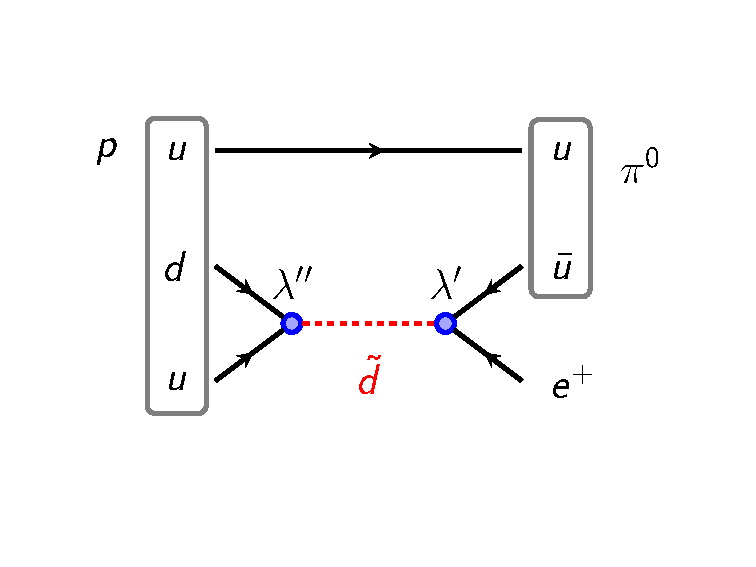
\includegraphics[
      width=\textwidth,
      clip=true,
      trim=1.5cm 1.5cm 1.5cm 1.5cm 
    ]
    {figures/theory/rpv_proton_decay.pdf}
    %%
    \\
    \vspace{5ex}
    %%
    \uncover<2->{
    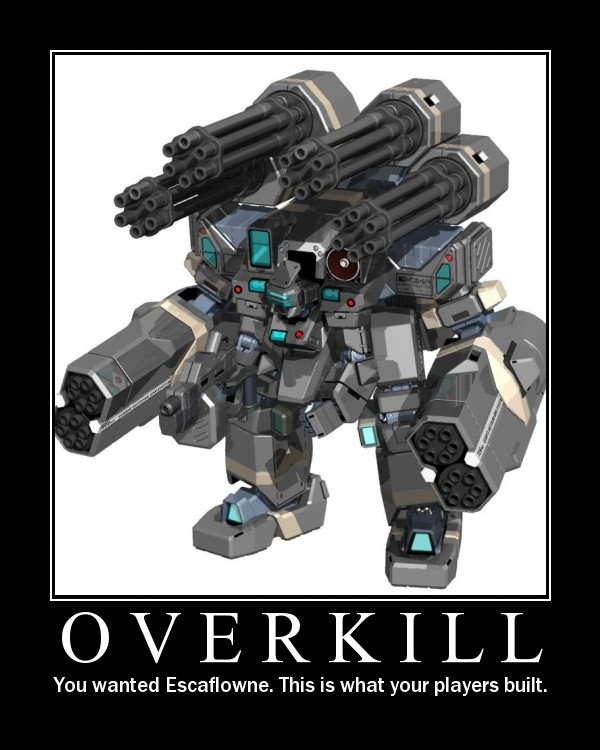
\includegraphics[
      width=\textwidth,
      clip=true,
      trim=0 0 0 0
    ]
    {figures/theory/overkill.jpg}
  }
  \end{columns}
  %%
\end{frame}


% ------------------------------------------------------------------------------
\begin{frame}
  \frametitle{Prevent proton decay?}
  %%
  \begin{center}
    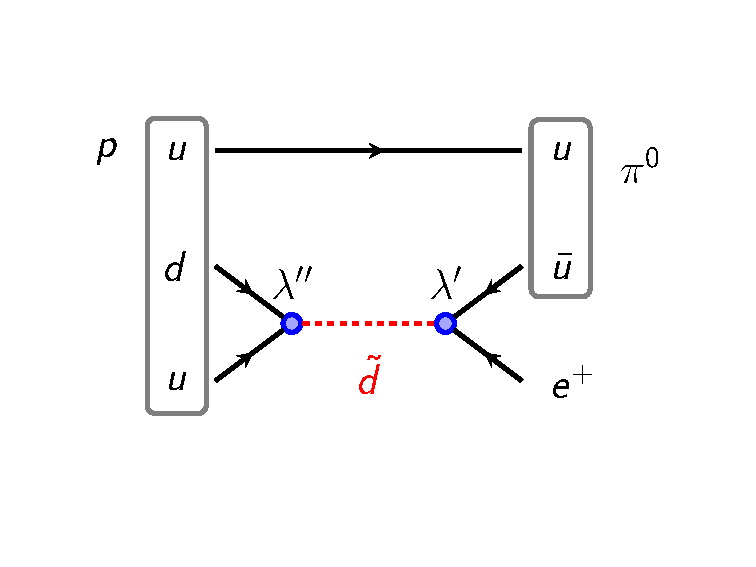
\includegraphics[
      width=0.6\textwidth,
      clip=true,
      trim=1.5cm 1.5cm 1.5cm 1.5cm 
    ]
    {figures/theory/rpv_proton_decay.pdf}
  \end{center}
  %%
  \begin{itemize}
    \item Proton decay requires both lepton number and baryon number violation 
    \item Sufficient to forbid one
  \end{itemize}
  %%
\end{frame}

% ==============================================================================
\subsection{\BMINUSL\ extension}

% ------------------------------------------------------------------------------
\begin{frame}
  \frametitle{\BMINUSL\ Extension}
  \begin{itemize}
    \item Introduce $U(1)_{B-L}$ symmetry group and right-handed neutrinos
    \item Prevents Baryon number violation
      \begin{itemize}
        \item Proton is safe!
        \item Lepton number violation is still allowed
      \end{itemize}
    \item SUSY particles can decay to SM particles
    \item LSP can have charge
      \begin{itemize}
        \item Stop is a possible LSP with unique signature
      \end{itemize}
  \end{itemize}
  %%
  \begin{columns}
    \column{0.60\linewidth}
    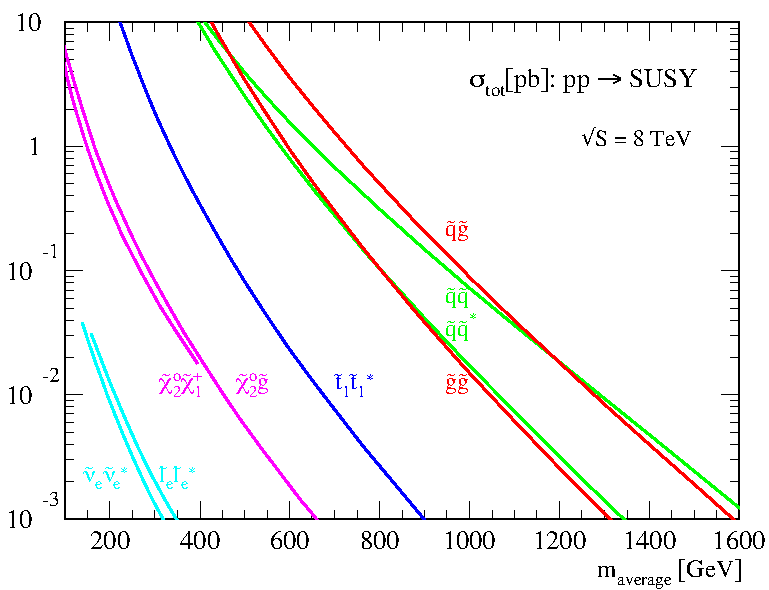
\includegraphics[width=\textwidth]{figures/theory/prospino_lhc8.pdf}
    %%
    \column{0.40\linewidth}
    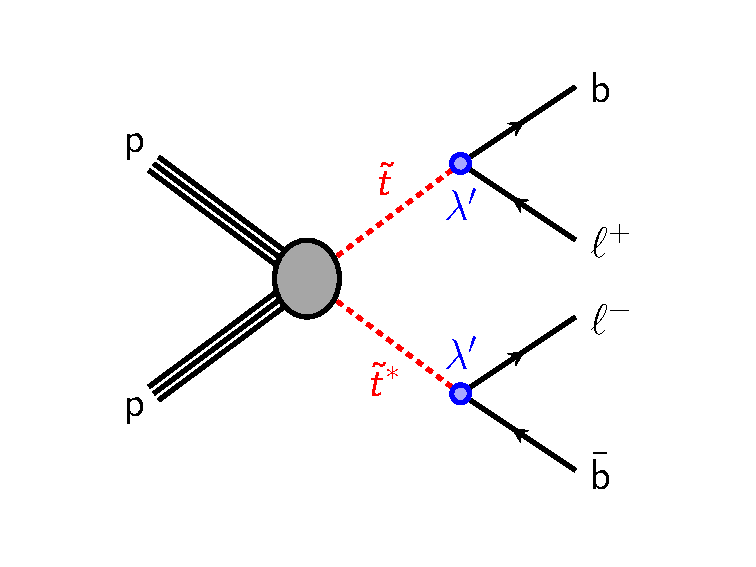
\includegraphics[
      width=\textwidth
    ]{figures/b_minus_l_stop_stop.pdf}
  \end{columns}
  %%
\end{frame}

%% %% % ------------------------------------------------------------------------------
%% \begin{frame}
%%   \frametitle{\BMINUSL\ \stop\ decays}
%%   %%
%%   \begin{itemize}
%%     % \item Decay of the LSP is related to the neutrino sector
%%     \item Look
%%     \item Differs from traditional leptoquark searches because decay can
%%       include $b$-quark and a \textbf{\color{nice_blue} light lepton}
%%     \item Previously, \textbf{\color{nice_blue}no direct search} for this model
%%     \item Results from leptoquark searches have been reinterpreted
%%   \end{itemize}
%%   %%
%%   \begin{center}
%%     \begin{tikzpicture}
%%       \node[
%%         anchor=south west,
%%         inner sep=0
%%       ] (image) at (0,0) {
%%         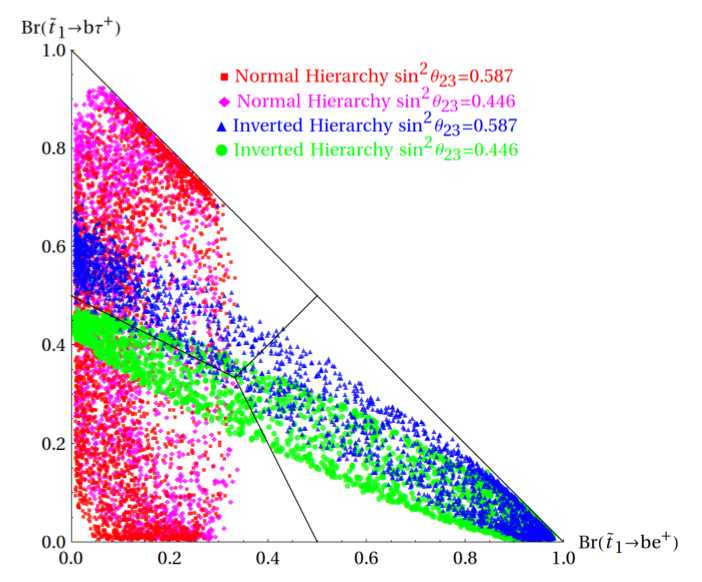
\includegraphics[width=0.55\linewidth]{figures/stop_model_scan.png}
%%         % 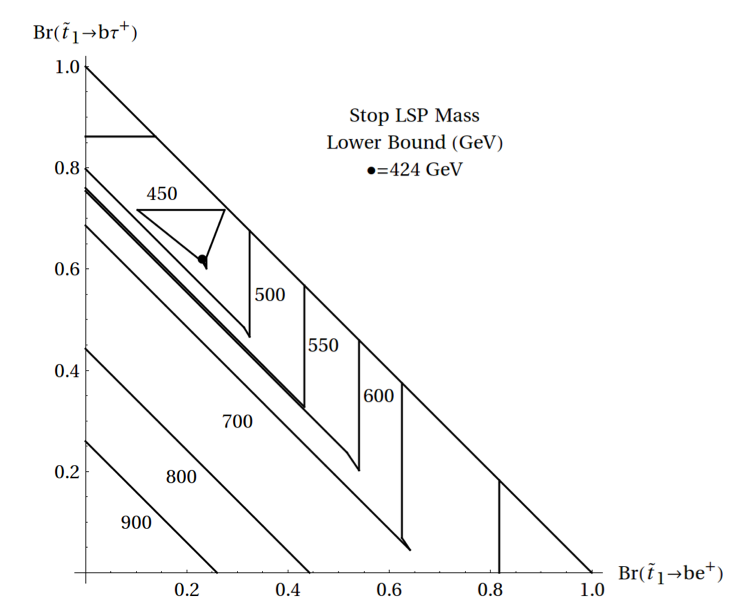
\includegraphics[width=0.60\textwidth]{figures/pheno_limit.png}
%%       };
%%       \begin{scope}[x={(image.south east)}, y={(image.north west)}]
%%         %% \node[rectangle,
%%         %%   rounded corners=1ex,
%%         %%   fill=RoyalBlue!30!white
%%         %% ] at (0.50, 0.95) {
%%         %%   \scriptsize
%%         %%   \href{http://arxiv.org/abs/1402.5434}{arxiv:1402.5434}
%%         %% };
%%         \node[
%%           rectangle,
%%           rounded corners=1ex,
%%           fill=RoyalBlue!80!white,
%%           text=white
%%         ] at (0.94, 0.15) {
%%           \small
%%           Mostly $b\,e$
%%         };
%%         \node[
%%           rectangle,
%%           rounded corners=1ex,
%%           fill=RoyalBlue!80!white,
%%           text=white
%%         ]
%%         at (-0.10, 0.15) {
%%           \small
%%           Mostly $b\,\mu$
%%         };
%%         %% \node[
%%         %%   rectangle,
%%         %%   rounded corners=1ex,
%%         %%   fill=ForestGreen!80!white,
%%         %%   text=white
%%         %% ]
%%         at (0.85, 0.5) {
%%           \footnotesize
%%           \begin{tabular}{c}
%%             Branching ratios of \\
%%             $\tilde{t}\rightarrow b\ell$ related to \\
%%             neutrino hierarchy
%%           \end{tabular}
%%         };
%%         %%
%%         \node[
%%           anchor=south east,
%%           inner sep=0
%%         ] (image) at (0.02,0.27) {
%%           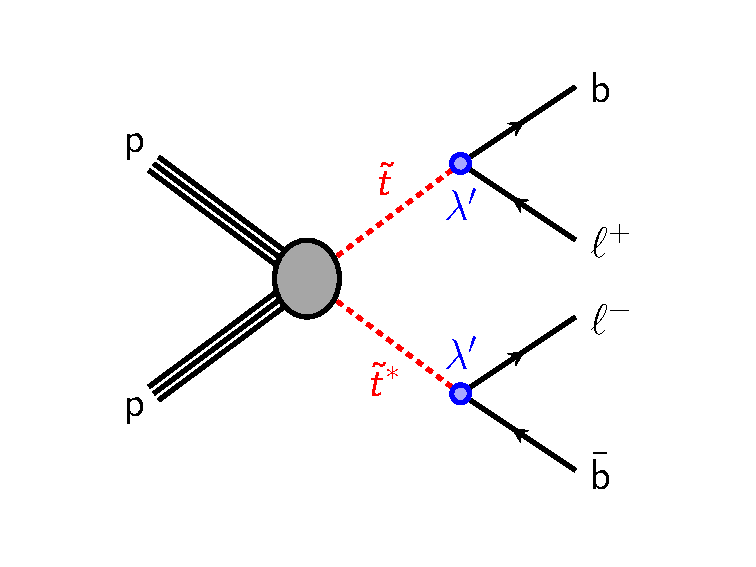
\includegraphics[width=0.4\linewidth]{figures/b_minus_l_stop_stop.pdf}
%%         };
%%         %%
%%         % \MyGrid
%%         %%
%%       \end{scope}
%%       %%
%%     \end{tikzpicture}
%%     % \end{columns}
%%   \end{center}
%%   %%
%% \end{frame}

%% % ------------------------------------------------------------------------------
%% \begin{frame}
%%   \frametitle{Previous results}
%%   %%
%%   \begin{itemize}
%%     \item Goal of this analysis is to
%%       % discover new particle \Simley{0.5} or
%%       % improve this limit \Simley{-0.5}
%%       \begin{itemize}
%%         \item discover new particle \Simley{0.5}
%%         \item or, improve this limit \Simley{-0.5}
%%       \end{itemize}
%%   \end{itemize}
%%   %%
%%   \begin{center}
%%     \begin{tikzpicture}
%%       \node[anchor=south west, inner sep=0] (image) at (0,0) {
%%         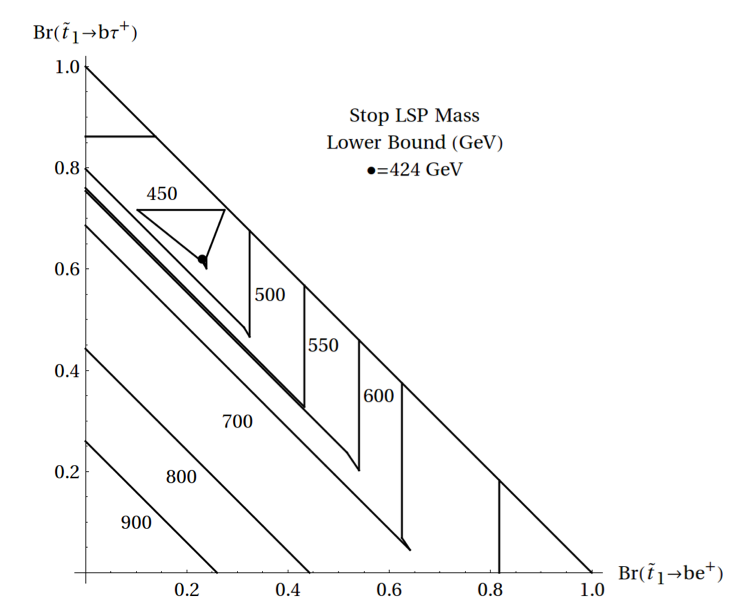
\includegraphics[width=0.6\textwidth]{figures/pheno_limit.png}
%%       };
%%       %% \begin{scope}[
%%       %%     x={(image.south east)},
%%       %%     y={(image.north west)}
%%       %%   ]
%%       %%   \node[
%%       %%     rectangle,
%%       %%     rounded corners=1ex,
%%       %%     fill=RoyalBlue!30!white
%%       %%   ]
%%       %%   at (0.50, 0.90) {
%%       %%     \scriptsize
%%       %%     \href{http://arxiv.org/abs/1402.5434}{arxiv:1402.5434}
%%       %%   };
%%       %%   %%
%%       %%   % \MyGrid
%%       %% \end{scope}
%%     \end{tikzpicture}
%%   \end{center}
%%   %%
%% \end{frame}

% ==============================================================================
\section{Experimental apparatus}
\subsection{Large Hadron Collider}

% ------------------------------------------------------------------------------
\begin{frame}
  \frametitle{Large Hadron Collider}
  %%
  \begin{center}
    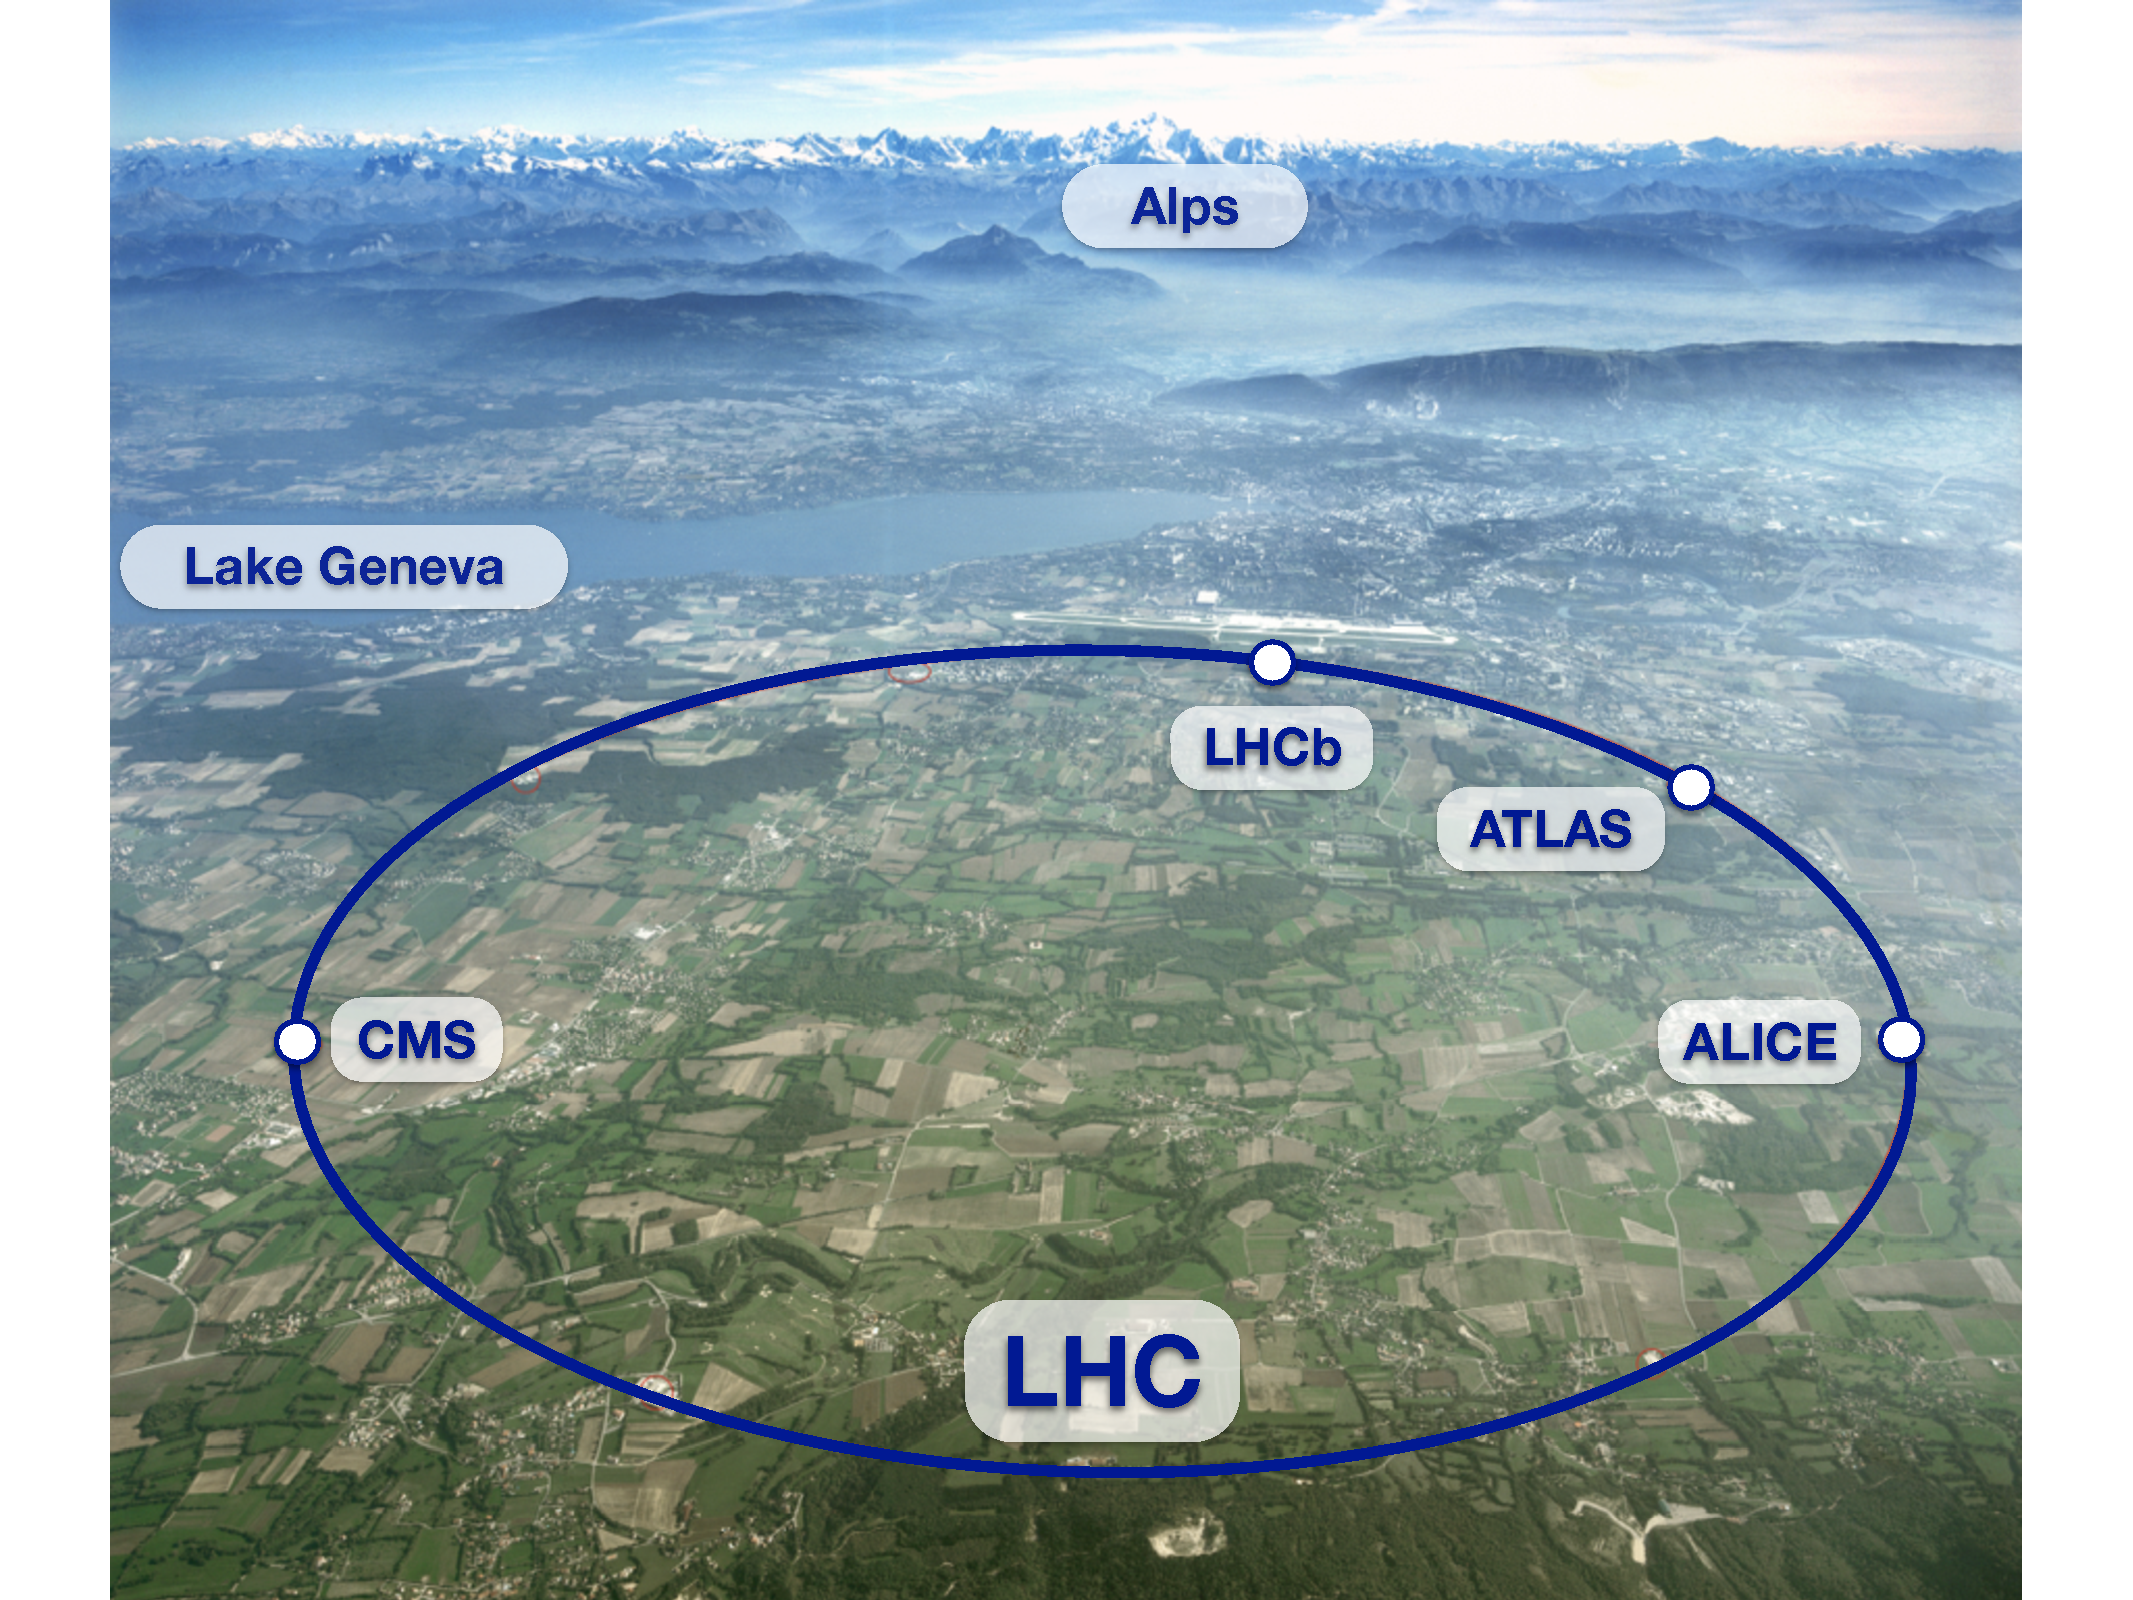
\includegraphics[width=0.95\textwidth]
    {figures/lhc_and_atlas/lhc_aerial.pdf}
  \end{center}
\end{frame}

% ------------------------------------------------------------------------------
\begin{frame}
  \frametitle{Large Hadron Collider}
  %%
  \begin{itemize}
    \item 27~km in circumference
    \item 8~\TeV\ center-of-mass energy
    \item 20.3~\ifb\ of $pp$ collision data in 2012
  \end{itemize}
  %%
  \begin{center}
    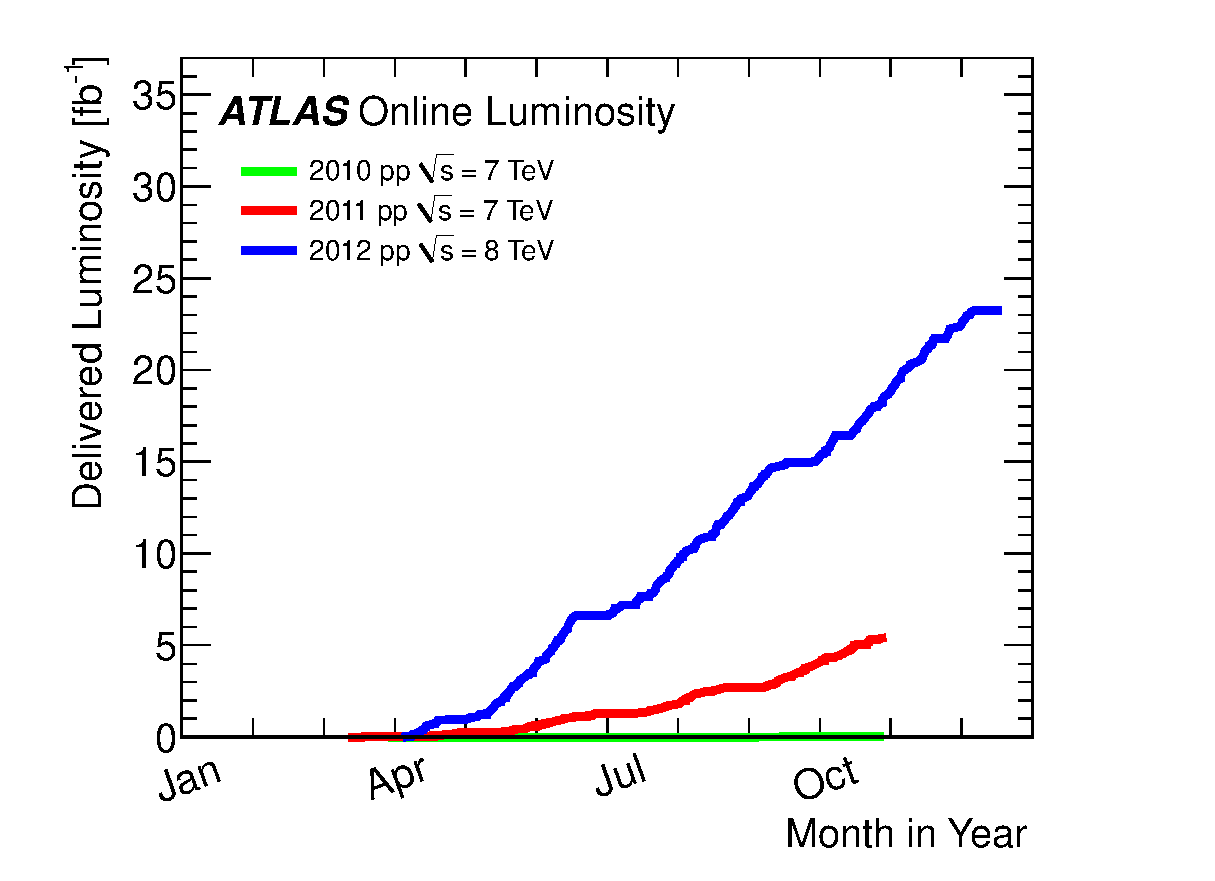
\includegraphics[width=0.8\textwidth]
    {figures/lhc_and_atlas/intlumivsyear.eps}
  \end{center}
\end{frame}

% ==============================================================================
\subsection{The \atlas\ experiment}

% ------------------------------------------------------------------------------
\begin{frame}
  \frametitle{\atlas}
  %%
  \begin{center}
    \includegraphics[width=\textwidth]
    {figures/lhc_and_atlas/atlas_det_dino_1.jpg}
  \end{center}
\end{frame}

% ------------------------------------------------------------------------------
\begin{frame}
  \frametitle{Particle signatures}
  %%
  \begin{center}
    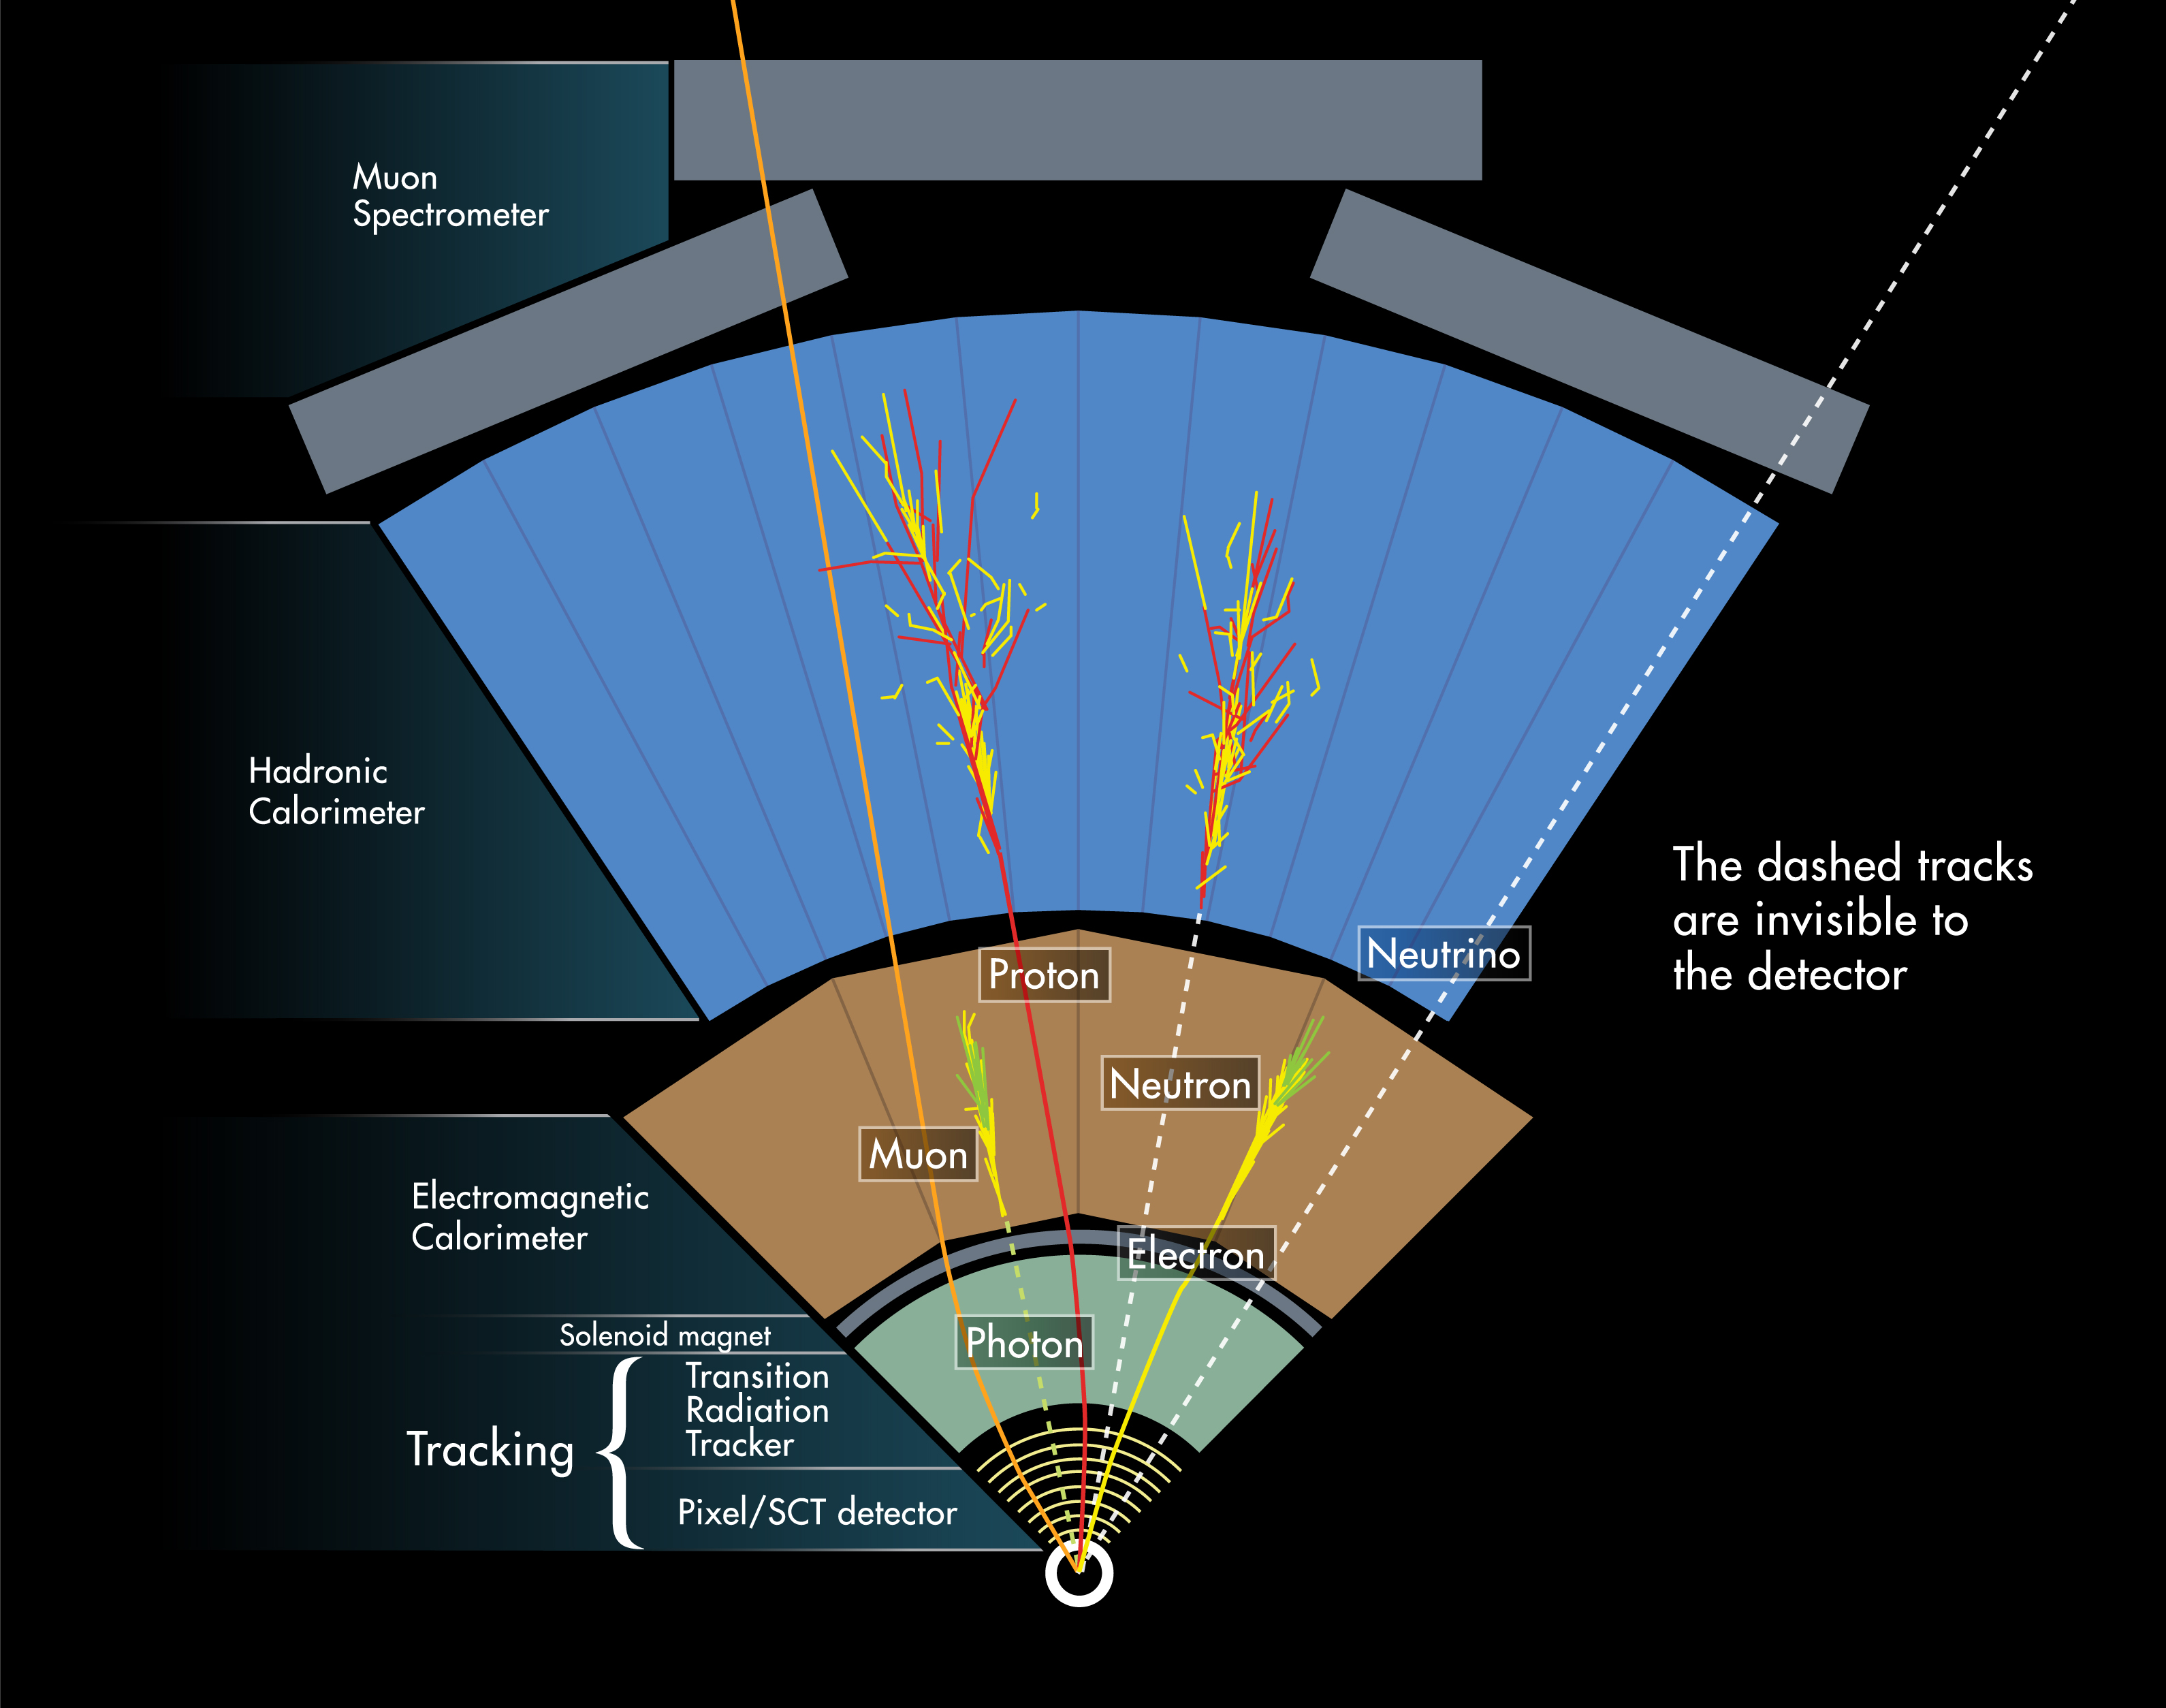
\includegraphics[width=0.95\textwidth]
    {figures/lhc_and_atlas/particle_signatures.jpg}
  \end{center}
\end{frame}

% ==============================================================================
\section{\BMINUSL\ search}
\subsection{Analysis strategy}

% ------------------------------------------------------------------------------
\begin{frame}
  \frametitle{Analysis strategy}
  %%
  \begin{itemize}
    \item Searching for stop pair production
      \begin{itemize}
        \item stops decay to
          {\color{nice_red} $b$-quark + lepton }
      \end{itemize}
      %%
    \item Interested in light leptons only
      \begin{itemize}
        \item Final states with
          {\color{nice_blue} $bbee$},
          {\color{nice_blue} $bb\mu\mu$}, or
          {\color{nice_blue} $bbe\mu$}
      \end{itemize}
      %%
    \item Signal expected to have resonance in invariant mass of
      $\ell+b$
      % lepton and $b$-quark
      %%
  \end{itemize}
  %%
  \begin{center}
    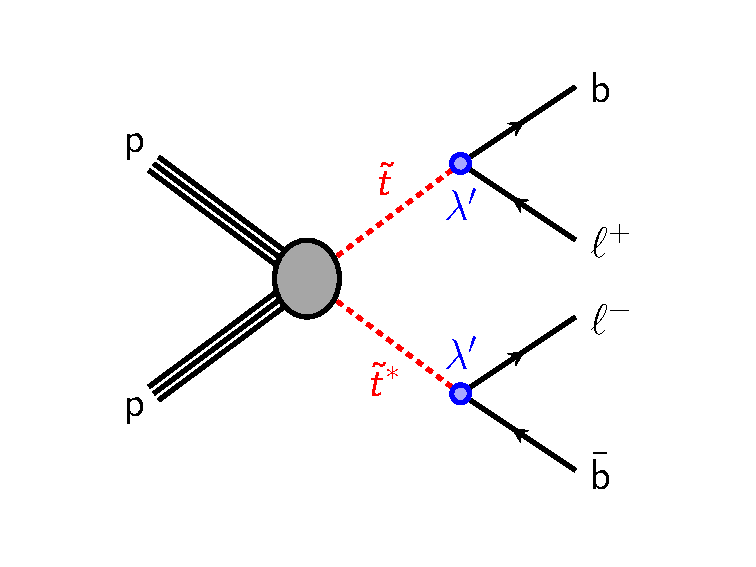
\includegraphics[width=0.5\textwidth]{figures/b_minus_l_stop_stop.pdf}
  \end{center}
\end{frame}

% ------------------------------------------------------------------------------
\begin{frame}
  \frametitle{Search strategy}
  %%
  \begin{columns}
    \column{0.6\textwidth}
    \begin{itemize}
      \item Selecting final states with
        \begin{itemize}
          \item {\color{nice_blue}Two leptons} ($e/\mu$)
          \item {\color{nice_red}Two $b$-tagged jets}
        \end{itemize}
        %%
      \item Define {\color{nice_blue}\textbf{two signal regions}} with high signal
        efficiency and low expected background contamination
        %%
      \item \textbf{\color{nice_red} Dedicated Control regions} to constrain
        \TTBAR\ and \ZGAMMA\ backgrounds
        %%
      \item Other backgrounds taken from MC
        %%
      %% \item For each choice of branching ratio, select region with the
      %%   {\color{nice_blue} \textbf{best expected sensitivity}}
        %%
    \end{itemize}
    %%
    \column{0.4\textwidth}
    \begin{block}{Signal}
      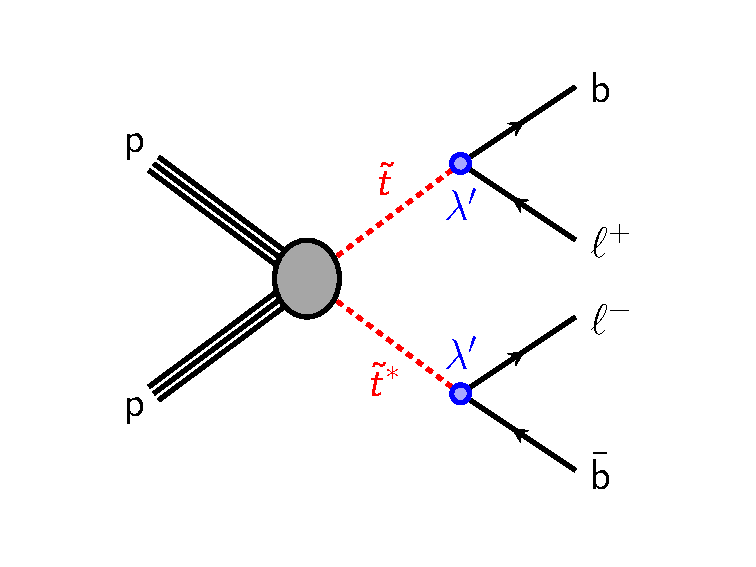
\includegraphics[width=\textwidth]{figures/b_minus_l_stop_stop.pdf}
    \end{block}
    \begin{block}{Background}
      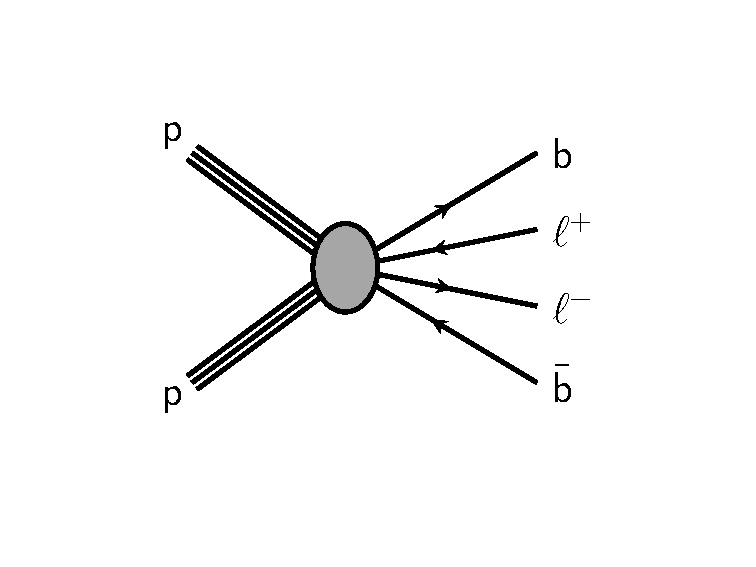
\includegraphics[width=\textwidth]{figures/generic_bbll.pdf}
    \end{block}
  \end{columns}
\end{frame}

%% % ------------------------------------------------------------------------------
%% \begin{frame}
%%   \frametitle{Monte Carlo signal samples}
%%   %%
%%   \begin{center}
%%     \begin{tikzpicture}
%%       \node[anchor=south west, inner sep=0] (image) at (0,0) {
%%         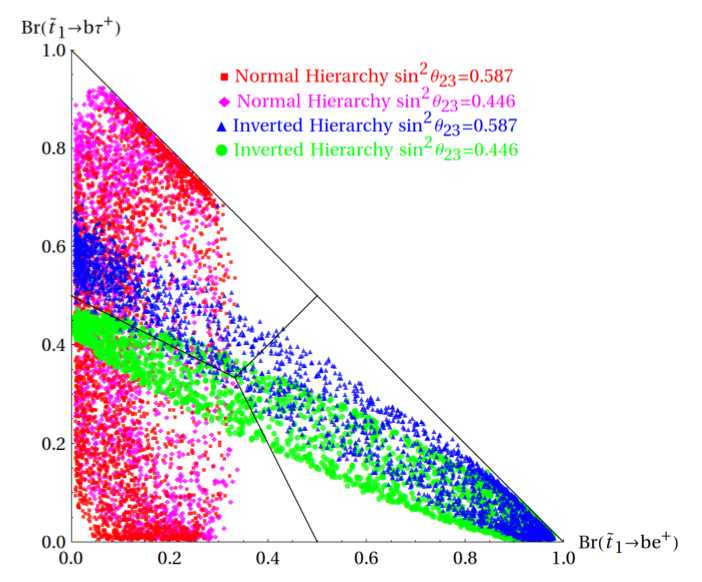
\includegraphics[width=0.55\linewidth]{figures/stop_model_scan.png}
%%       };
%%       \begin{scope}[
%%           x={(image.south east)}, y={(image.north west)}
%%         ]
%%         \fill[
%%           fill=MidnightBlue!80!white
%%         ]
%%         (0.45,0.075)
%%         circle
%%         (0.5ex);
%%         %
%%         \node[
%%           rectangle,
%%           rounded corners=1ex,
%%           fill=nice_blue,
%%           text=white
%%         ]
%%         at (0.94, 0.15) {
%%           \small
%%           Mostly $bbee$
%%         };
%%         %
%%         \node[
%%           rectangle,
%%           rounded corners=1ex,
%%           fill=nice_blue,
%%           text=white
%%         ]
%%         at (-0.10, 0.15)
%%         {
%%           \small
%%           Mostly $bb\mu\mu$
%%         };
%%         \node[
%%           rectangle,
%%           rounded corners=1ex,
%%           fill=ForestGreen!80!white,
%%           text=white
%%         ]
%%         at (0.93, 0.5) {
%%           \footnotesize
%%           \begin{tabular}{c}
%%             Increasing the \\
%%             branching ratio to \\
%%             $b\tau$ leads to fewer \\
%%             observable events
%%           \end{tabular}
%%         };
%%         \draw[
%%           -stealth,
%%           ForestGreen!80!white,
%%           ultra thick
%%         ]
%%         (0.65, 0.3) to (0.40, 0.60);
%%         %%
%%         \node[
%%           anchor=south east,
%%           inner sep=0
%%         ] (image) at (0.02,0.27) {
%%           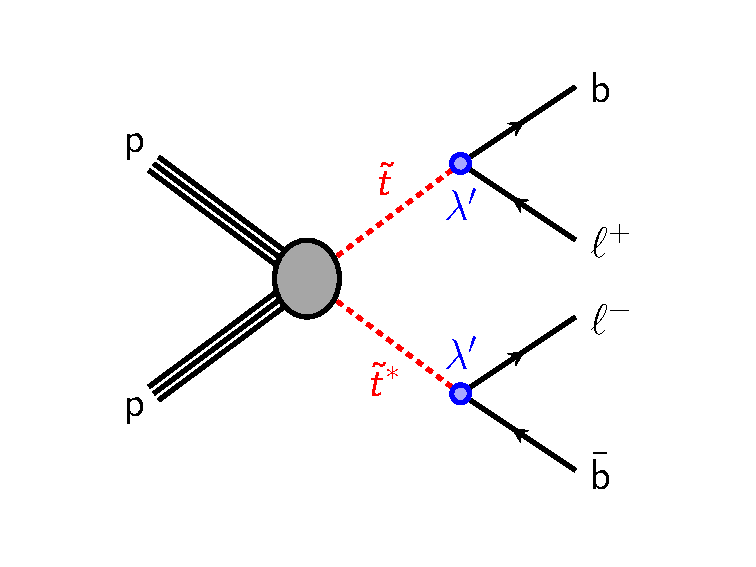
\includegraphics[width=0.4\linewidth]{figures/b_minus_l_stop_stop.pdf}
%%         };
%%         %%
%%         % \MyGrid
%%       \end{scope}
%%     \end{tikzpicture}
%%   \end{center}
%%   %%
%%   \begin{itemize}
%%     \item Monte Carlo samples used to optimize selection and interpret results
%%     \item Stop mases from 400~\GeV\ to 1.1~\TeV
%%     \item Cross sections at NLO
%%     \item $Br(\stop \rightarrow be) = Br(\stop \rightarrow b\mu) = 0.5$
%%   \end{itemize}
%%   %%
%% \end{frame}


% ------------------------------------------------------------------------------
\begin{frame}
  \frametitle{Object selection}
  %%
  \begin{itemize}
    \item Electrons, muons, and jets required to have $\pt > 40 \GeV$
    % \item Remove overlap between objects
    \item At least two leptons with opposite charge and two $b$-tagged jets
      \begin{itemize}
        \item Select two leading lepton and two leading b-tagged jets if
          there are more than two of each
      \end{itemize}
    \item Two possible pairings for $bb\ell\ell$ system
      \begin{center}
        \resizebox{0.80\textwidth}{!}{%
          \begin{tikzpicture}
            \node[rectangle, text=black] (sel1) at (-5.0,+0.5) {Selection 1:};
            \node[rectangle, text=black] (sel2) at (-5.0,-0.5) {Selection 2:};

            \node[rectangle, rounded corners=1ex, fill=pairing_b_1, text=black] (b1) at (-3.25,+0.5) {$b_1$};
            \node[rectangle, rounded corners=1ex, fill=pairing_l_1, text=black] (l1) at (-2.50,+0.5) {$\ell_1$};
            \node[rectangle, rounded corners=1ex, fill=pairing_b_2, text=black] (b2) at (+1.25,+0.5) {$b_2$};
            \node[rectangle, rounded corners=1ex, fill=pairing_l_2, text=black] (l2) at (+2.00,+0.5) {$\ell_2$};
            \node[rectangle, text=black] (m11) at (-1.0,+0.5) {$\Rightarrow m_{b1\ell1} = m_{b\ell}^{0}$};
            \node[rectangle, text=black] (m22) at (+3.5,+0.5) {$\Rightarrow m_{b2\ell2} = m_{b\ell}^{1}$};

            \node[rectangle, rounded corners=1ex, fill=pairing_b_1, text=black] (b1) at (-3.25,-0.5) {$b_1$};
            \node[rectangle, rounded corners=1ex, fill=pairing_l_2, text=black] (l2) at (-2.50,-0.5) {$\ell_2$};
            \node[rectangle, rounded corners=1ex, fill=pairing_b_2, text=black] (b2) at (+1.25,-0.5) {$b_2$};
            \node[rectangle, rounded corners=1ex, fill=pairing_l_1, text=black] (l1) at (+2.00,-0.5) {$\ell_1$};
            \node[rectangle, text=black] (m12) at (-1.0,-0.5) {$\Rightarrow m_{b1\ell2} = m_{b\ell}^{0} $};
            \node[rectangle, text=black] (m21) at (+3.5,-0.5) {$\Rightarrow m_{b2\ell1} = m_{b\ell}^{1} $};
          \end{tikzpicture}
        }
      \end{center}
    \item Expect masses signal-like masses to be the same
    \item Choose pairing with smallest difference in mass between two pairs
  \end{itemize}
  %%
\end{frame}


% ------------------------------------------------------------------------------
\begin{frame}
  \frametitle{Selection criteria}
  %%
  \begin{itemize}
      % \item[Major backgrounds:] \TTBAR, \ZGAMMAJETS, Single top production
    \item \textbf{\color{nice_blue} Major backgrounds:} \TTBAR, \ZGAMMAJETS, Single top production
  \end{itemize}
  \vspace{1ex}
  \begin{description}
      % \item[Major backgrounds:] \TTBAR, \ZGAMMAJETS, Single top production
    \item[\MLL:] \ZJETS\ has narrow resonance in \MLL\ near the 
      $m_Z$
      \begin{itemize}
        \item Apply ``$Z$-veto'' to reject \ZJETS\ events
        \item Same flavor leptons with $|\MLL - m_Z| \leq 10 \GeV$
      \end{itemize}
      %%
    \item[\HT:] Decay products from massive stops have high-\pt
      \begin{itemize}
        \item Decay products from SM parents have lower \pt
        \item Require scalar sum of the \pt\ of the two $b$-tagged jets and
          the two leptons be $\geq 1100 \GeV$
      \end{itemize}
      %%
    \item[\MBLASYM:] Resonant decay of stop
      \begin{itemize}
        \item Small difference in \MBL\ of two pairs for stop decay
        \item Difference can be large in SM decays like \TTBAR
        \item Require
          $\nicefrac{\left(\MBL^0-\MBL^1\right)}{\left(\MBL^0+\MBL^1\right)}
          \leq 0.2$
      \end{itemize}
      %%
    \item[$\MBL^0$:] Massive stop has large \MBL
      \begin{itemize}
        \item Distinguish signal regions using $\MBL^0$
        \item $\MBL^0 \geq 400 \GeV$ and $\MBL^0 \geq 600 \GeV$
      \end{itemize}
  \end{description}
\end{frame}


%% % ------------------------------------------------------------------------------
%% \begin{frame}[t]
%%   \frametitle{Signal regions}
%%   \begin{columns}[t]
%%     \column{0.46\textwidth}
%%     \begin{block}{\HT}
%%       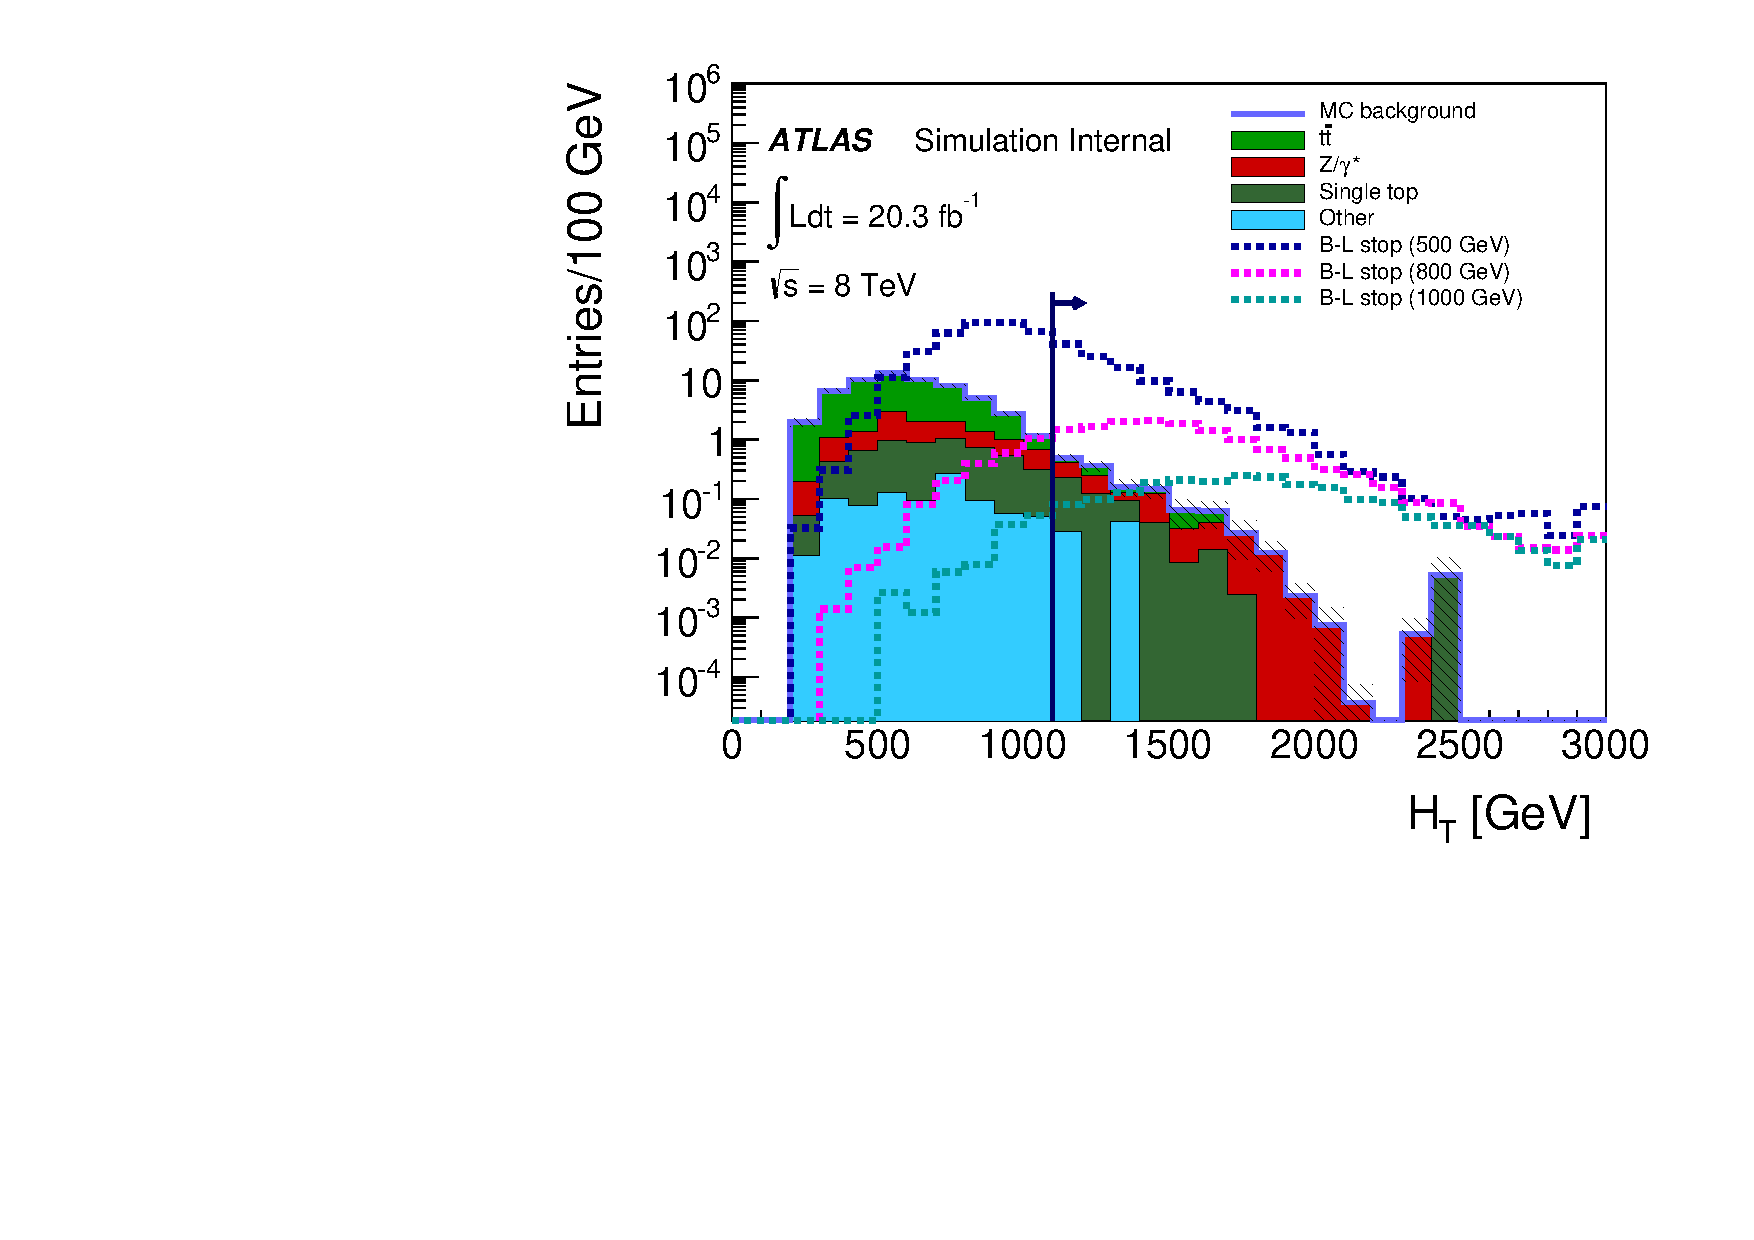
\includegraphics[width=\textwidth]{figures/ht_sr_400_minus_ht.pdf}
%%     \end{block}
%%     \begin{block}{\MBLASYM}
%%       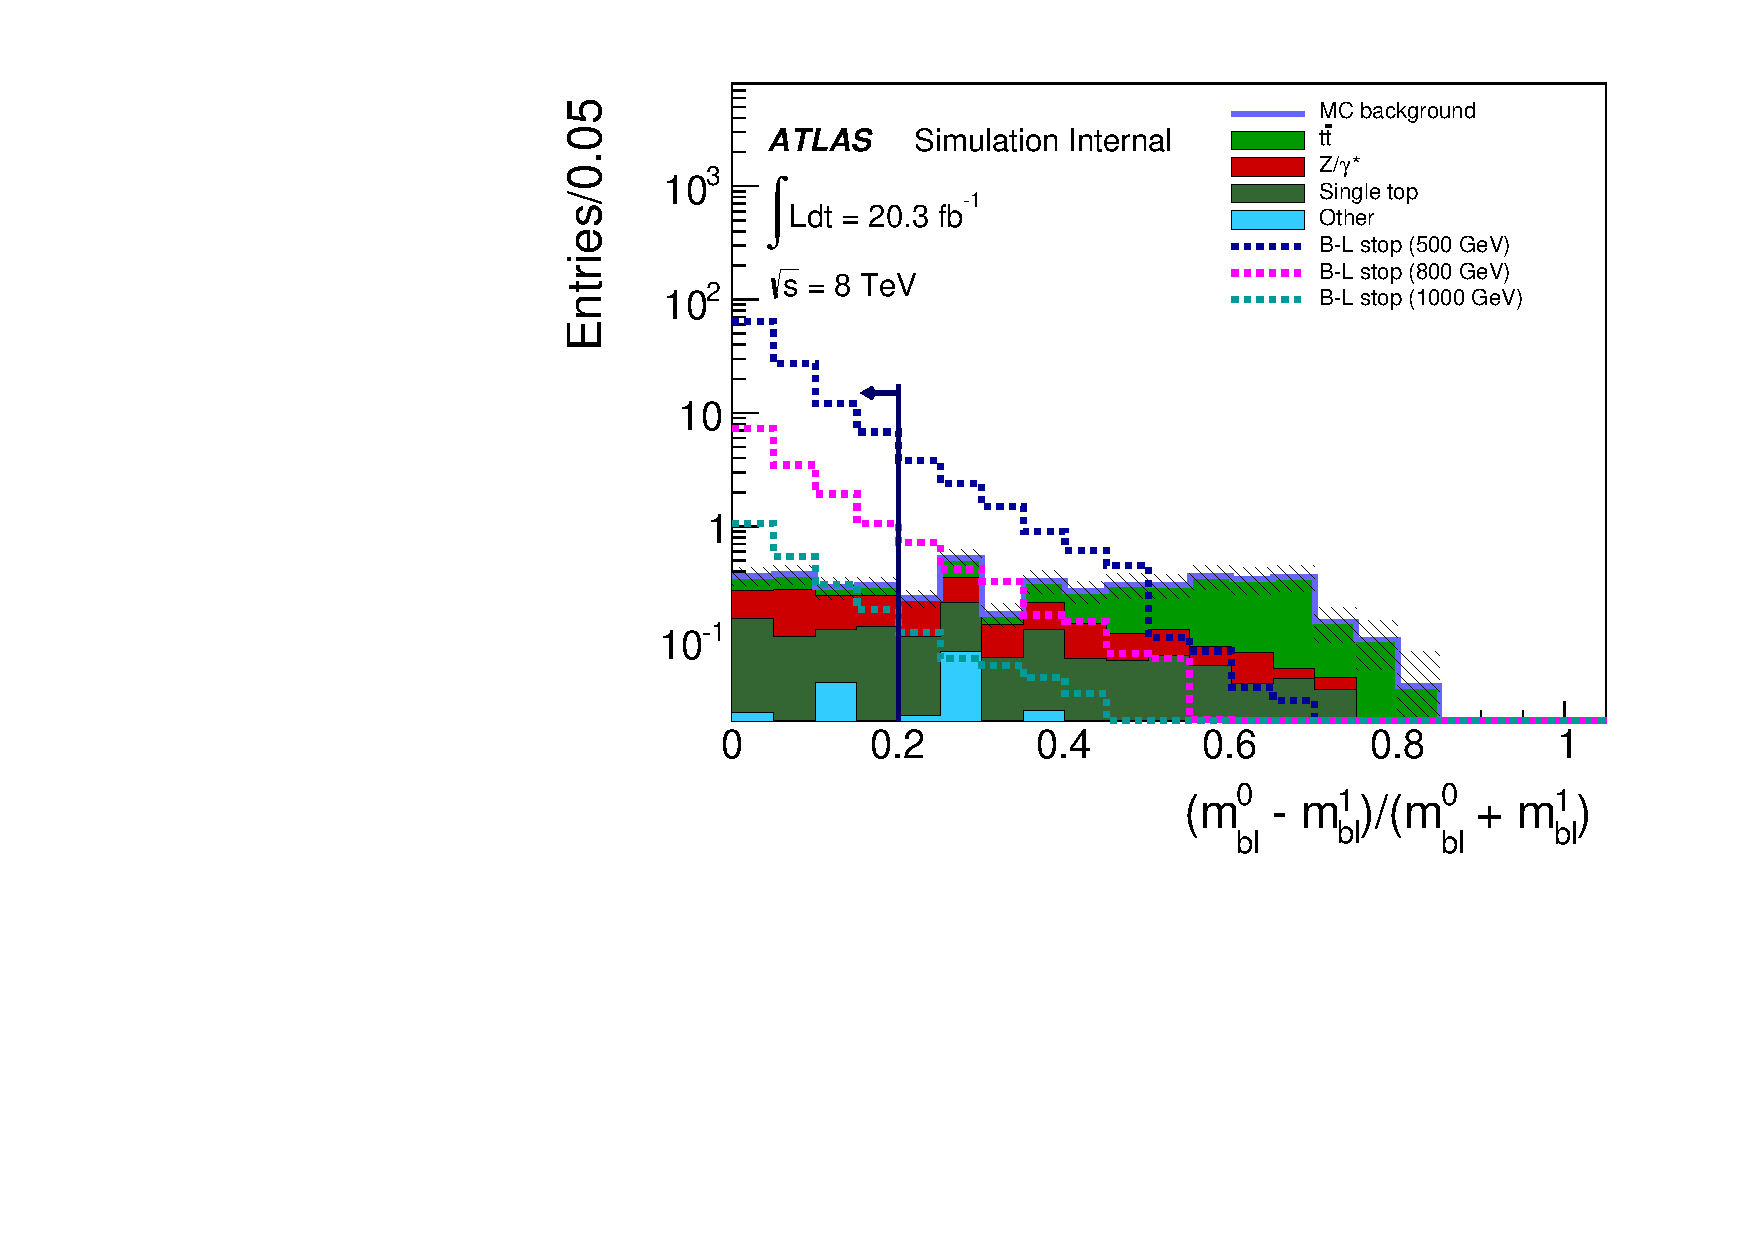
\includegraphics[width=\textwidth]{figures/mbl_asym_sr_400_minus_mbl_asym.pdf}
%%     \end{block}
%%     %%
%%     \column{0.50\textwidth}
%%     \begin{block}{$\MBL^0$}
%%       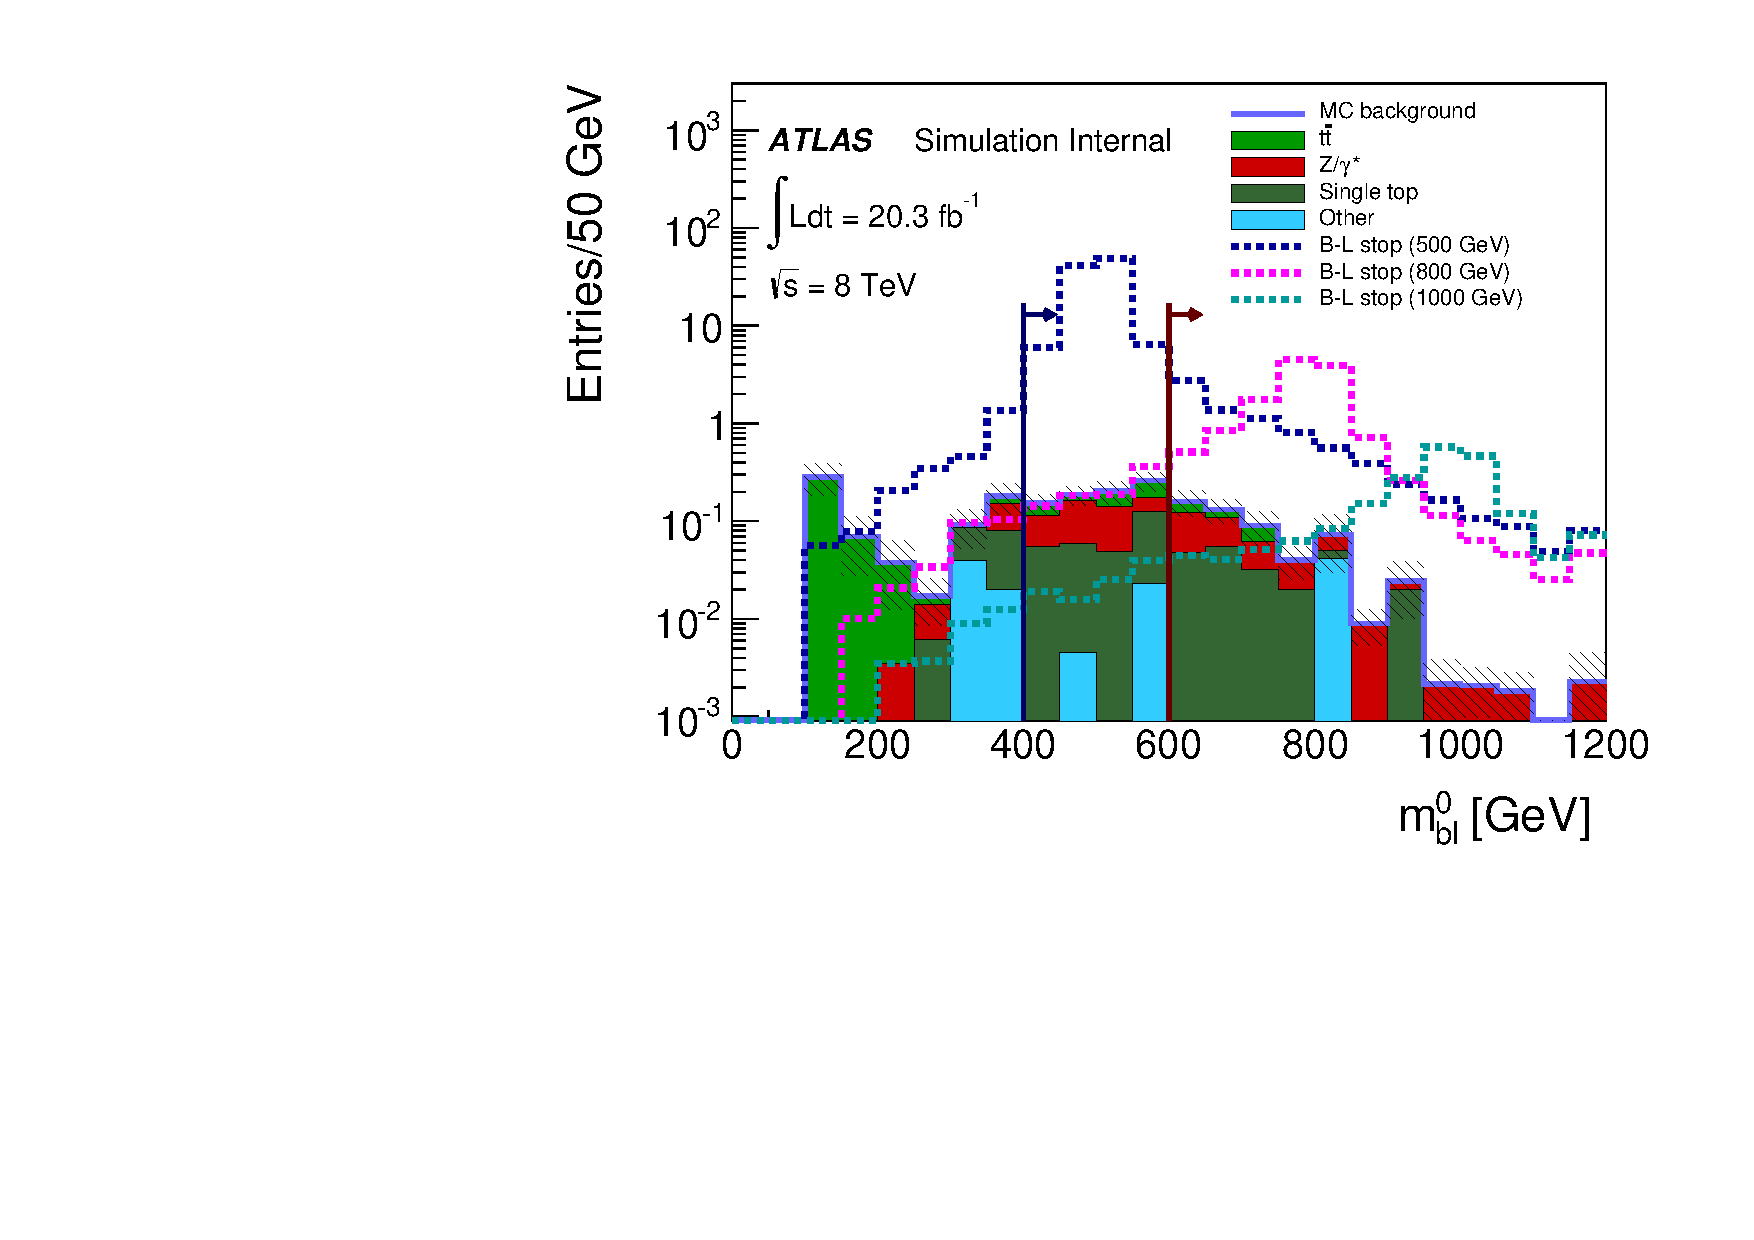
\includegraphics[width=\textwidth]{figures/mbl_0_sr_minus_mbl.pdf}
%%     \end{block}
%%     %%
%%     \begin{itemize}
%%       % \item Expected distributions when applying all but one of the signal
%%       %   region cuts
%%       \item Expected distributions: all but one of the SR cuts
%%       \item Left plots apply cut of $\MBL \ge 400$
%%       % \item \HT\ and \MBLASYM\ plots apply a cut of $\MBL \ge 400$
%%     \end{itemize}
%%   \end{columns}
%% \end{frame}


% ------------------------------------------------------------------------------
\begin{frame}[t]
  \frametitle{Signal regions}
  \begin{columns}
    \column{0.50\textwidth}
    % \begin{block}{\HT}
      \begin{center}
        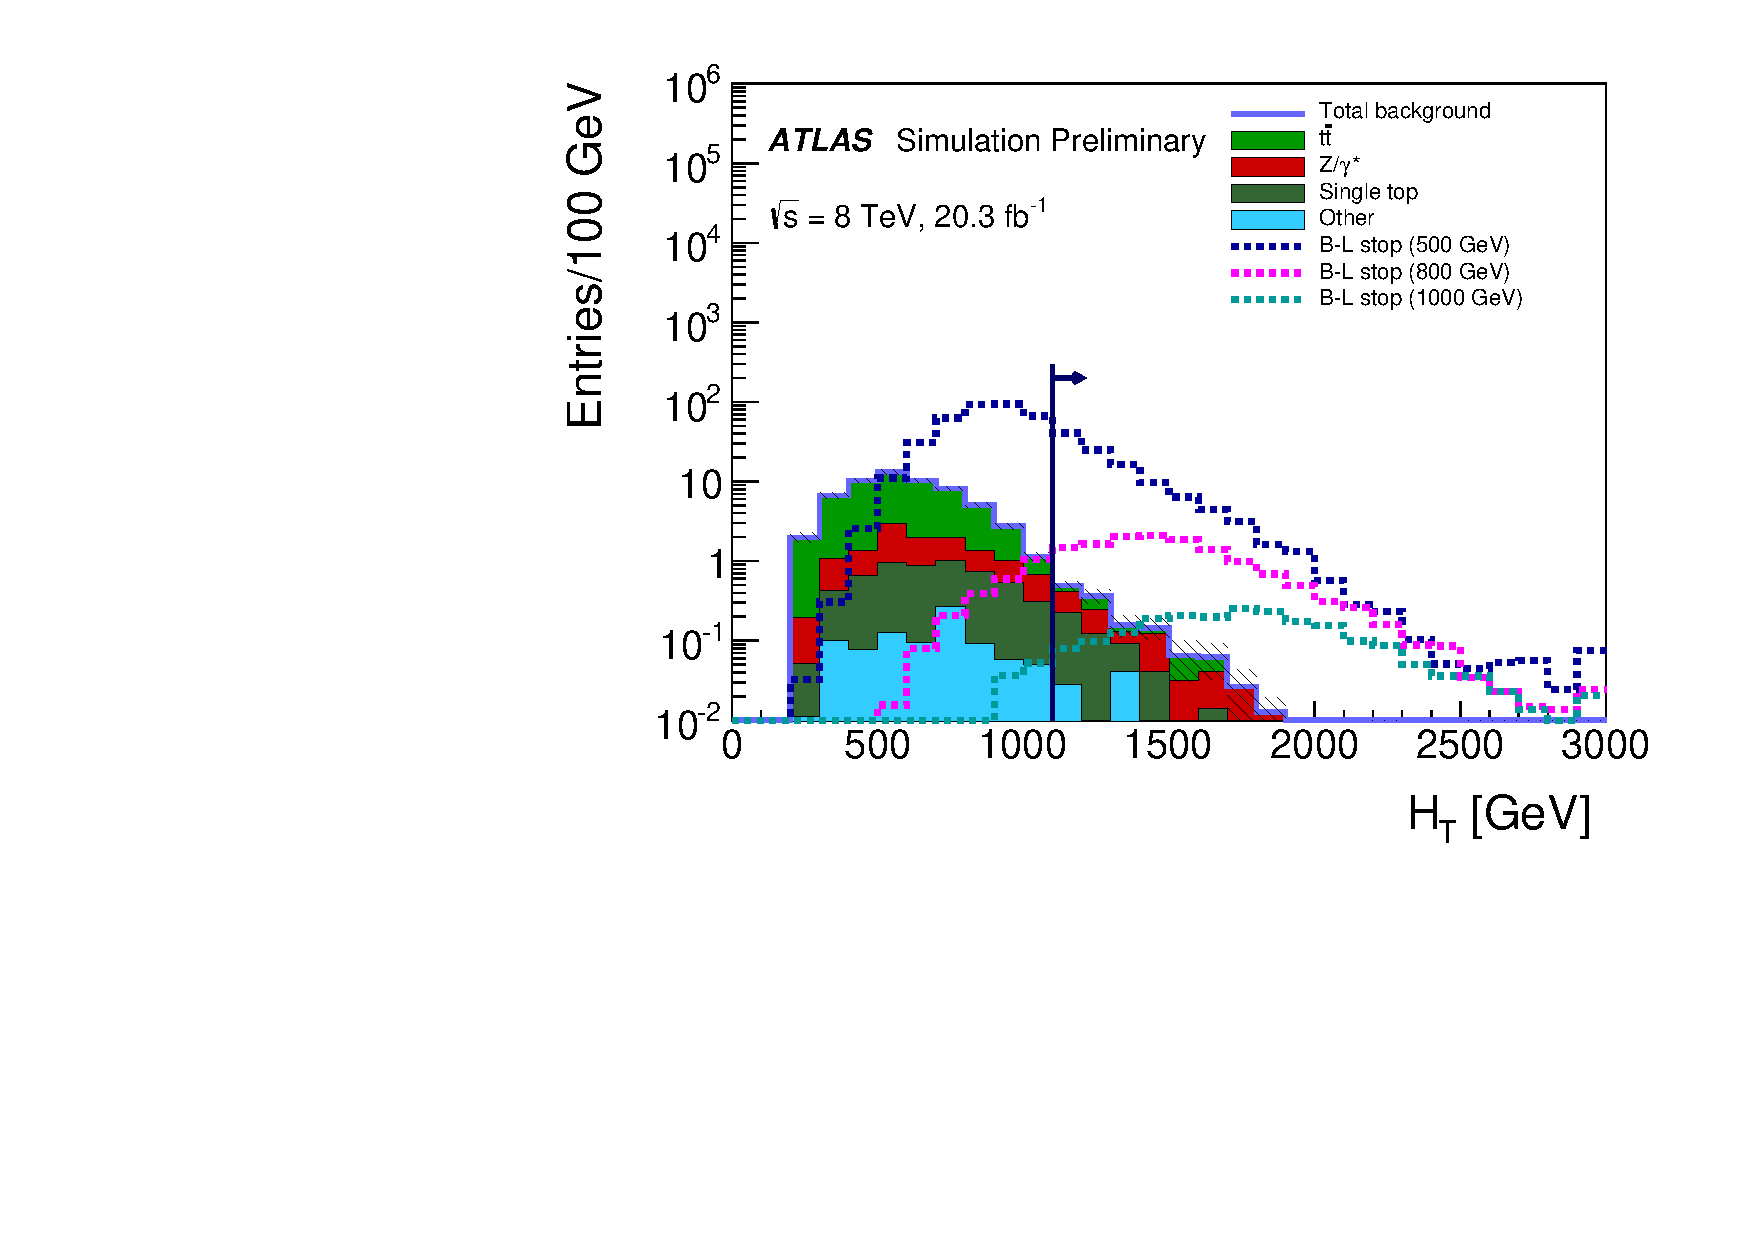
\includegraphics[width=0.92\textwidth]{figures/blstop/ht_sr_400_minus_ht.pdf}
        \\
        % \end{block}
        % \begin{block}{\MBLASYM}
        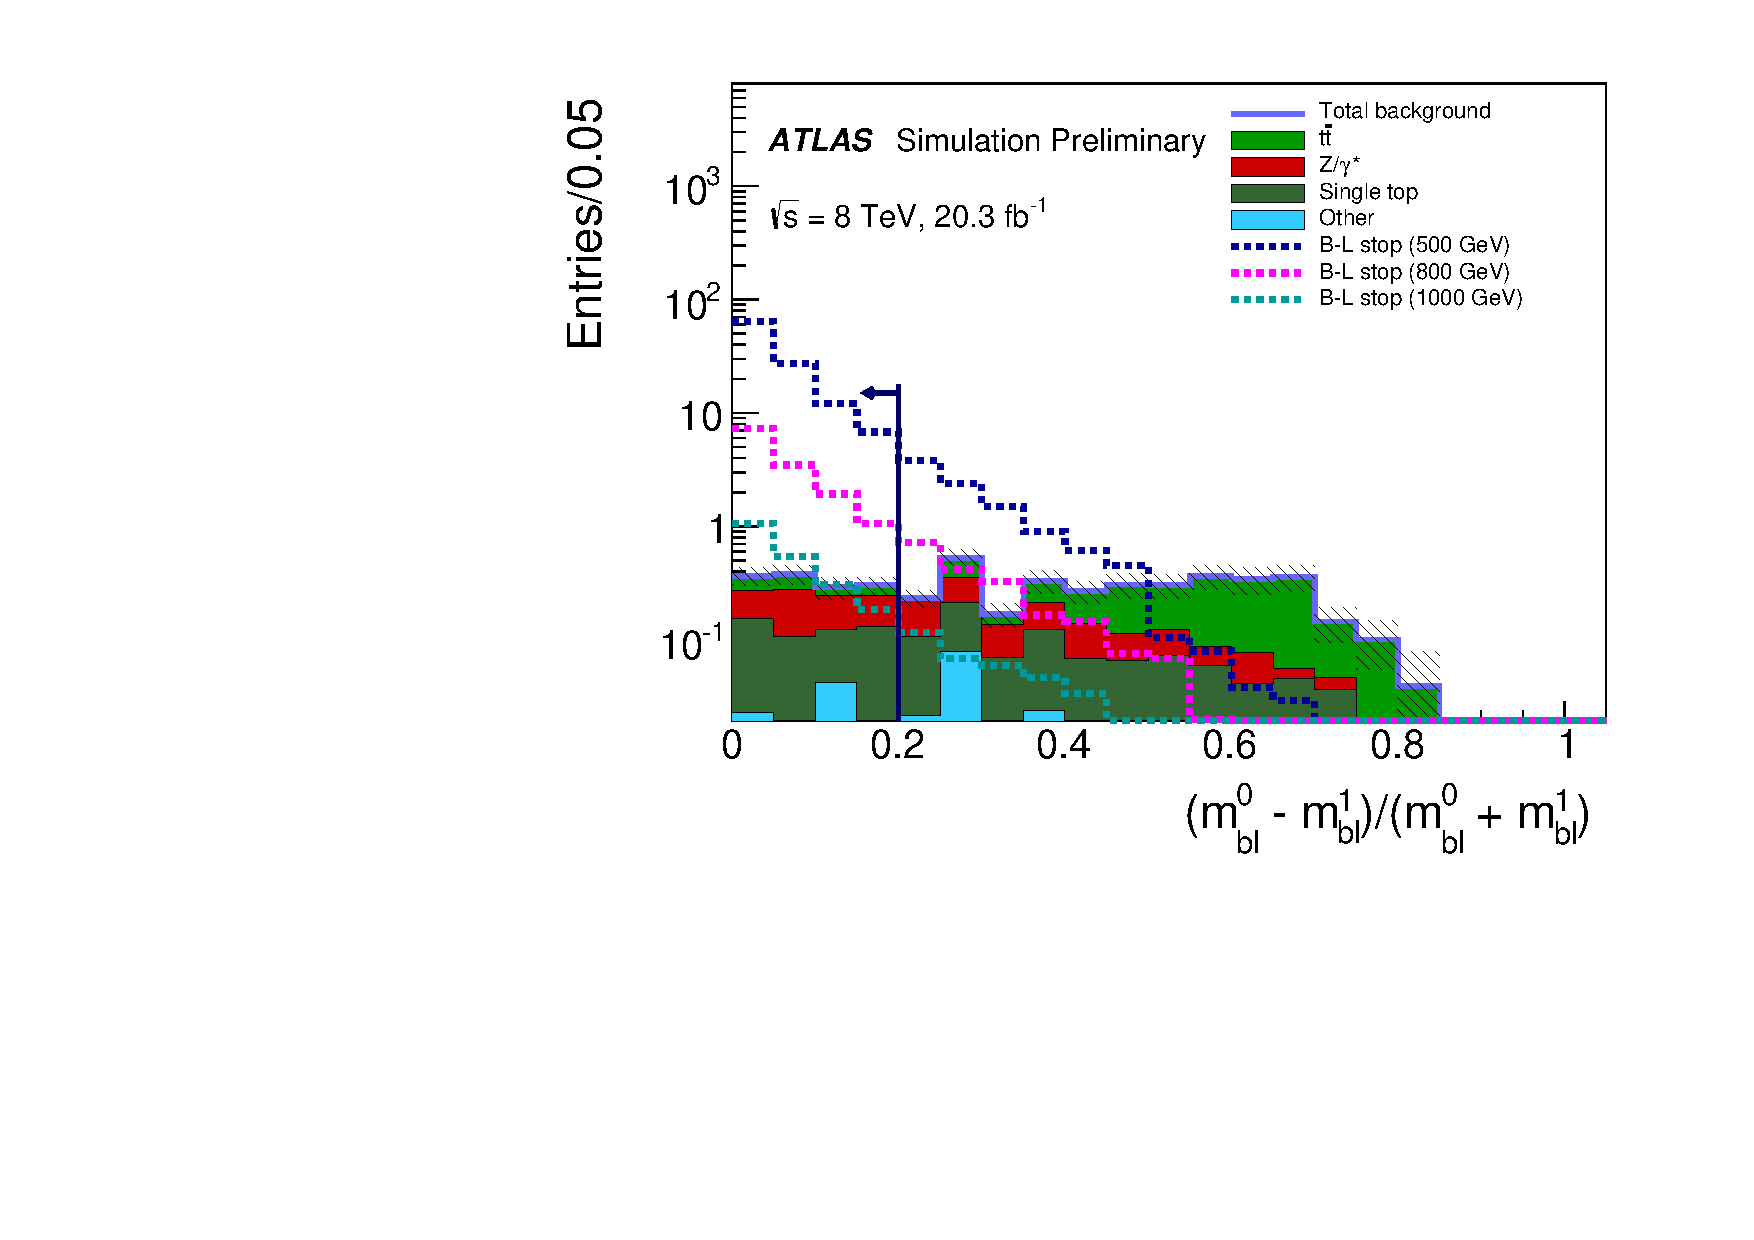
\includegraphics[width=0.92\textwidth]{figures/blstop/mbl_asym_sr_400_minus_mbl_asym.pdf}
      \end{center}
      % \end{block}
    %%
    \column{0.50\textwidth}
    % \begin{block}{$\MBL^0$}
      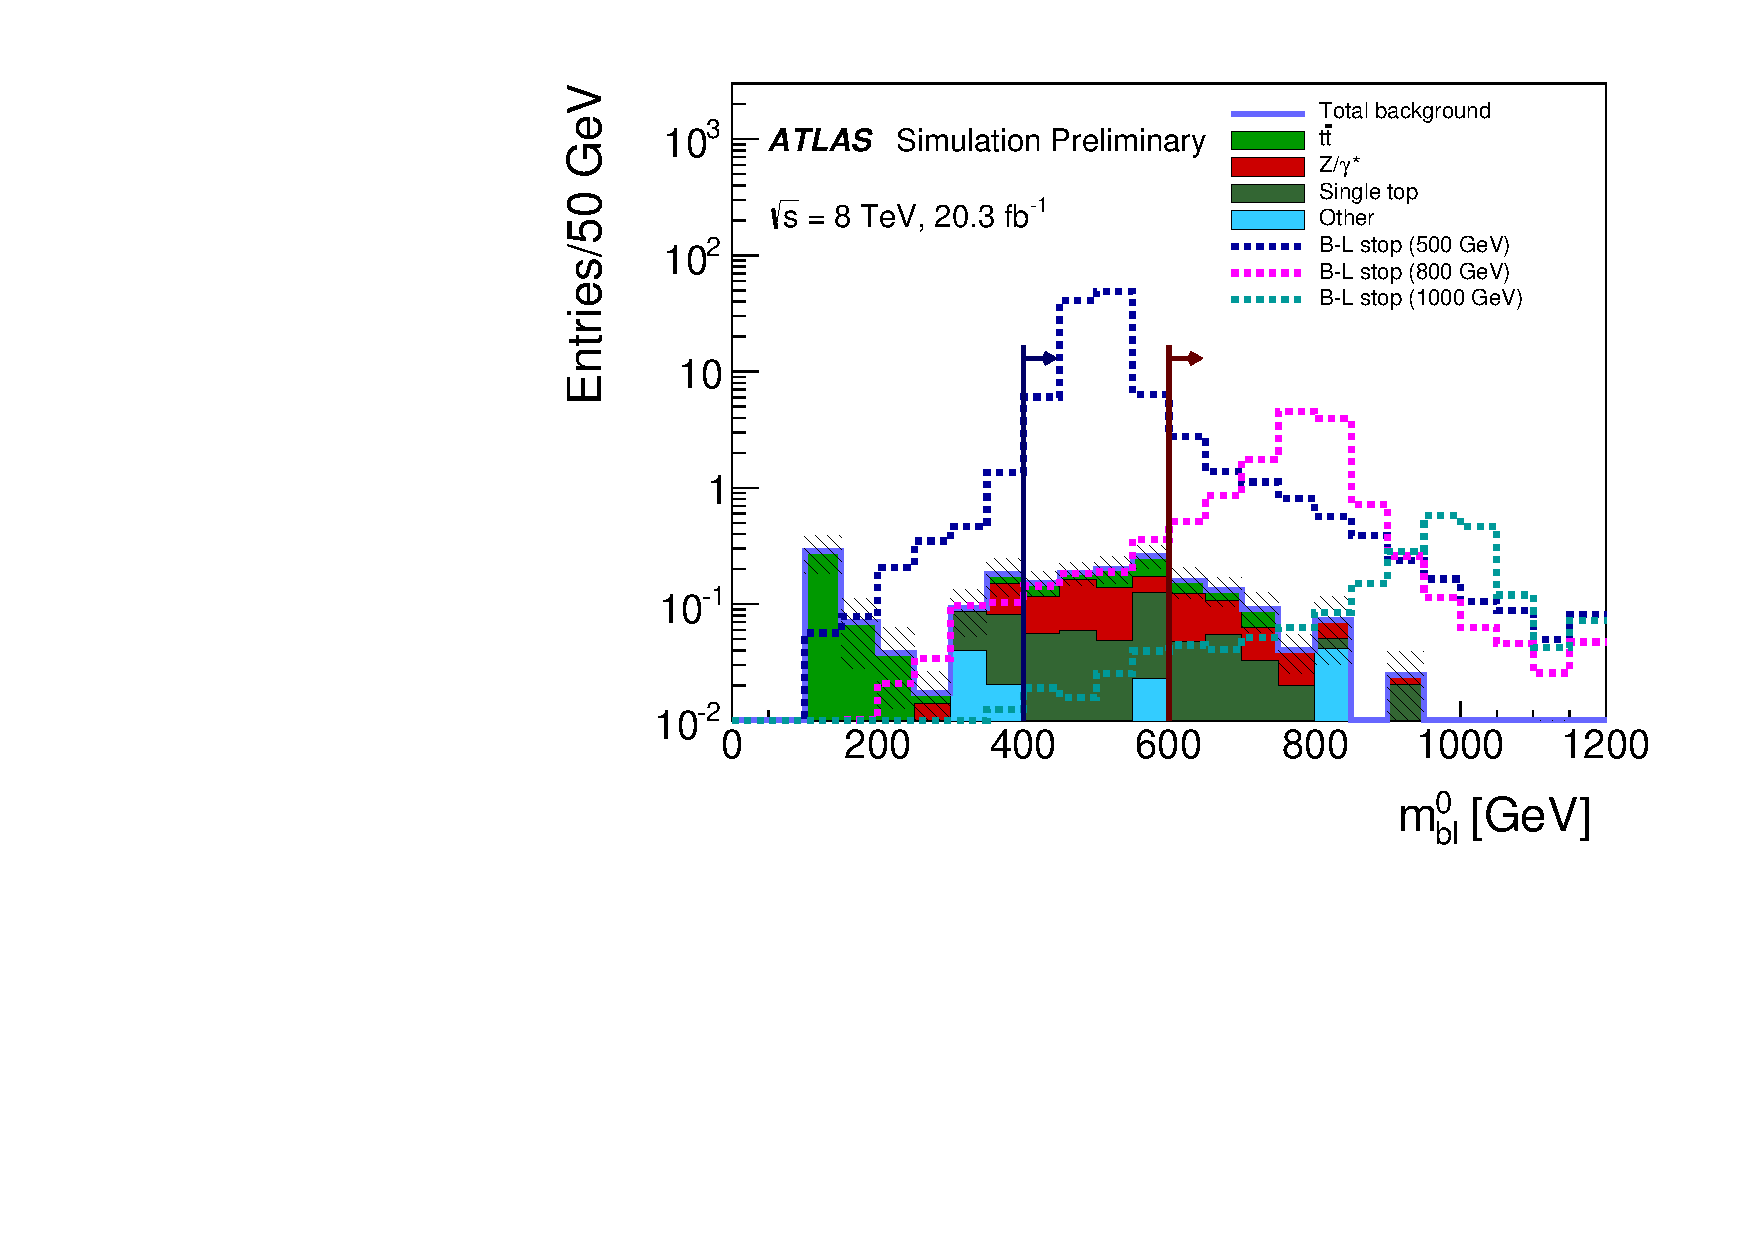
\includegraphics[width=\textwidth]{figures/blstop/mbl_0_sr_minus_mbl.pdf}
    % \end{block}
    %%
    \begin{itemize}
      % \item Expected distributions when applying all but one of the signal
      %   region cuts
      \item Expected distributions: all but one of the SR cuts
      \item Left plots apply cut of $\MBL \ge 400$
      % \item \HT\ and \MBLASYM\ plots apply a cut of $\MBL \ge 400$
    \end{itemize}
  \end{columns}
\end{frame}



% ==============================================================================
\subsection{Background estimate}

% ------------------------------------------------------------------------------
\begin{frame}
  \frametitle{Background estimate}
  %%
  \begin{itemize}
    \item Construct control regions for \TTBAR\ and \ZGAMMAJETS
      \begin{description}
        \item[Top CR] Low \HT, high \MET, $Z$-veto
        \item[$Z$ CR] Low \HT, low \MET, select $Z$-window
      \end{description}
    \item Determine normalization from maximum likelihood fit to data
    \item Other backgrounds taken from Monte Carlo simulation
    \item Validation regions for extrapolation from control regions to other
      kinematic regions
  \end{itemize}
\end{frame}


% ------------------------------------------------------------------------------
\frame[t]
{
  \frametitle{Region definitions}
  \begin{columns}
    \column{0.6\linewidth}
    \begin{figure}
      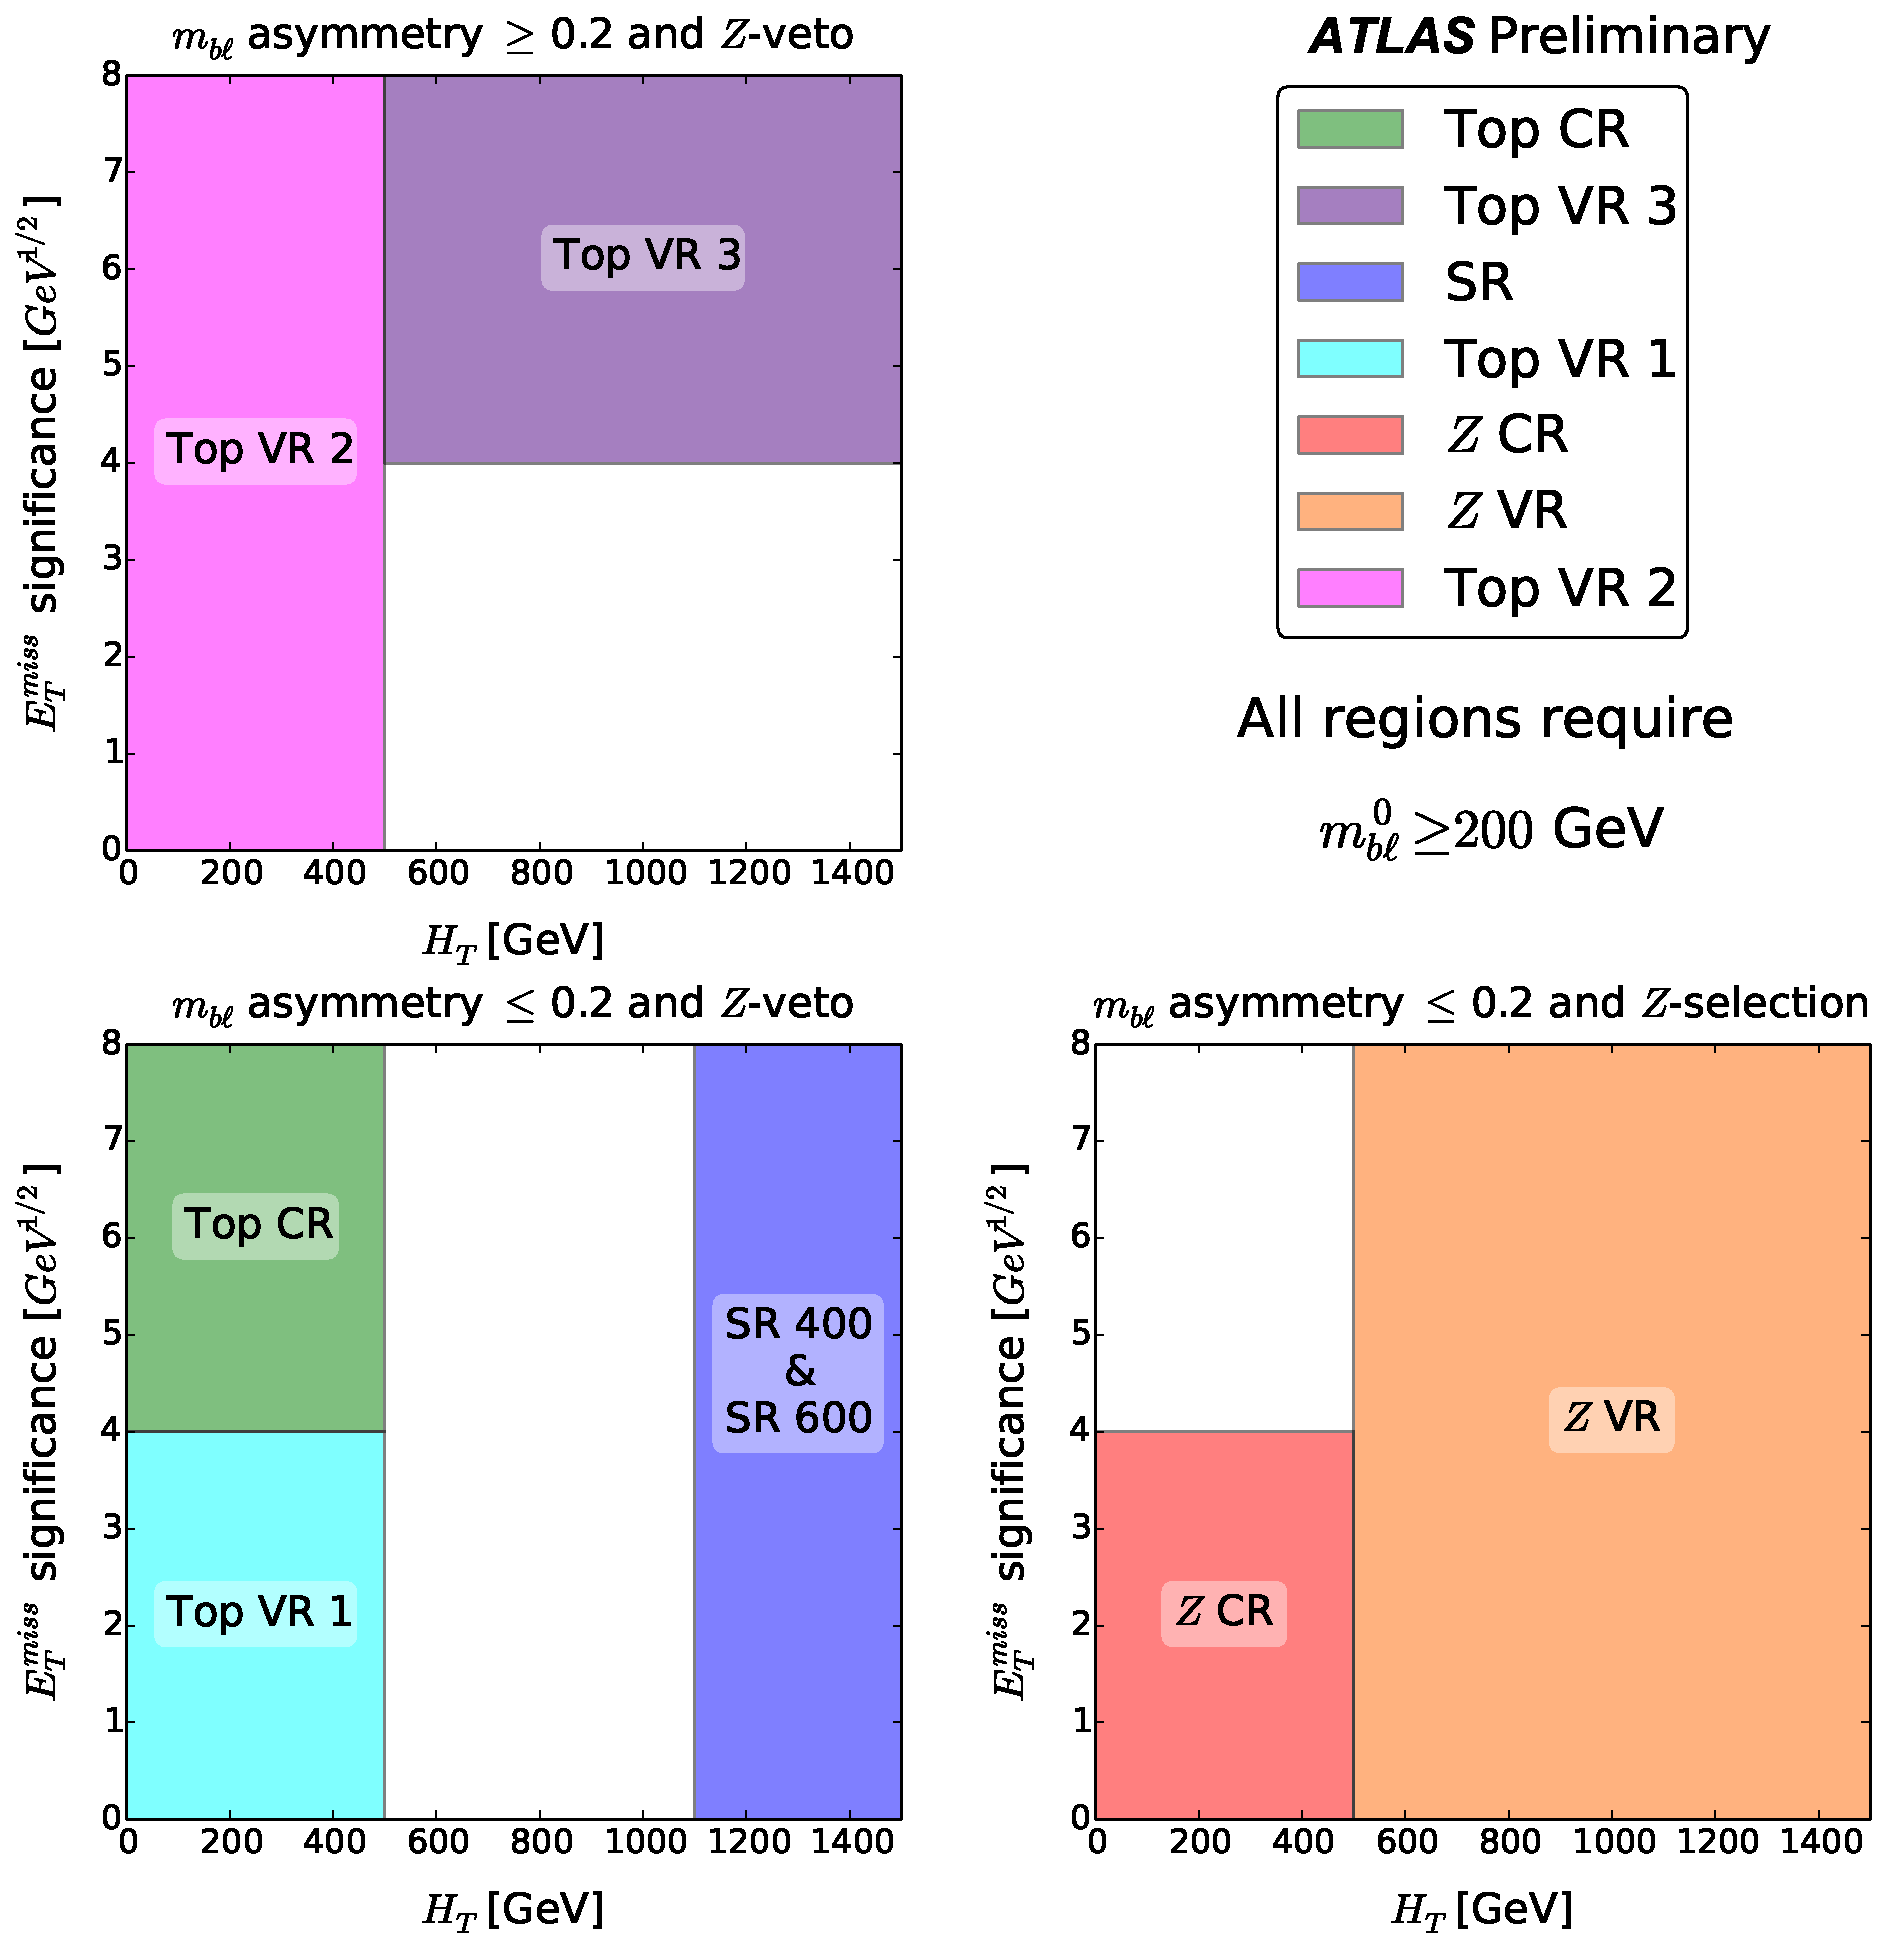
\includegraphics[width=\textwidth]
      {figures/blstop/regions__met_sig__ht_plane.pdf}
    \end{figure}
    %%
    \column{0.4\linewidth}
    \begin{itemize}
      \item $Z$ region: $ee$ or $\mu\mu$ with
        $|m_{\ell\ell} - m_Z| \le 10 \GeV$
    \end{itemize}
    \vspace{1ex}
    \[
      \HT = \sum_{i=1}^{2} p_T^{\ell_i} + \sum_{j=1}^{2} p_T^{b \mathrm{~jet}_j}
    \]
    \vspace{1ex}
    \[
      \MBLASYM = 
      \frac{\left(\MBL^0-\MBL^1\right)}{\left(\MBL^0+\MBL^1\right)}
    \]
    \vspace{1ex}
    \[
      \METSIG = \frac{\MET}{\sqrt{\HT}}
    \]
  \end{columns}
}


% ------------------------------------------------------------------------------
\begin{frame}
  \frametitle{Background estimate: control regions}
  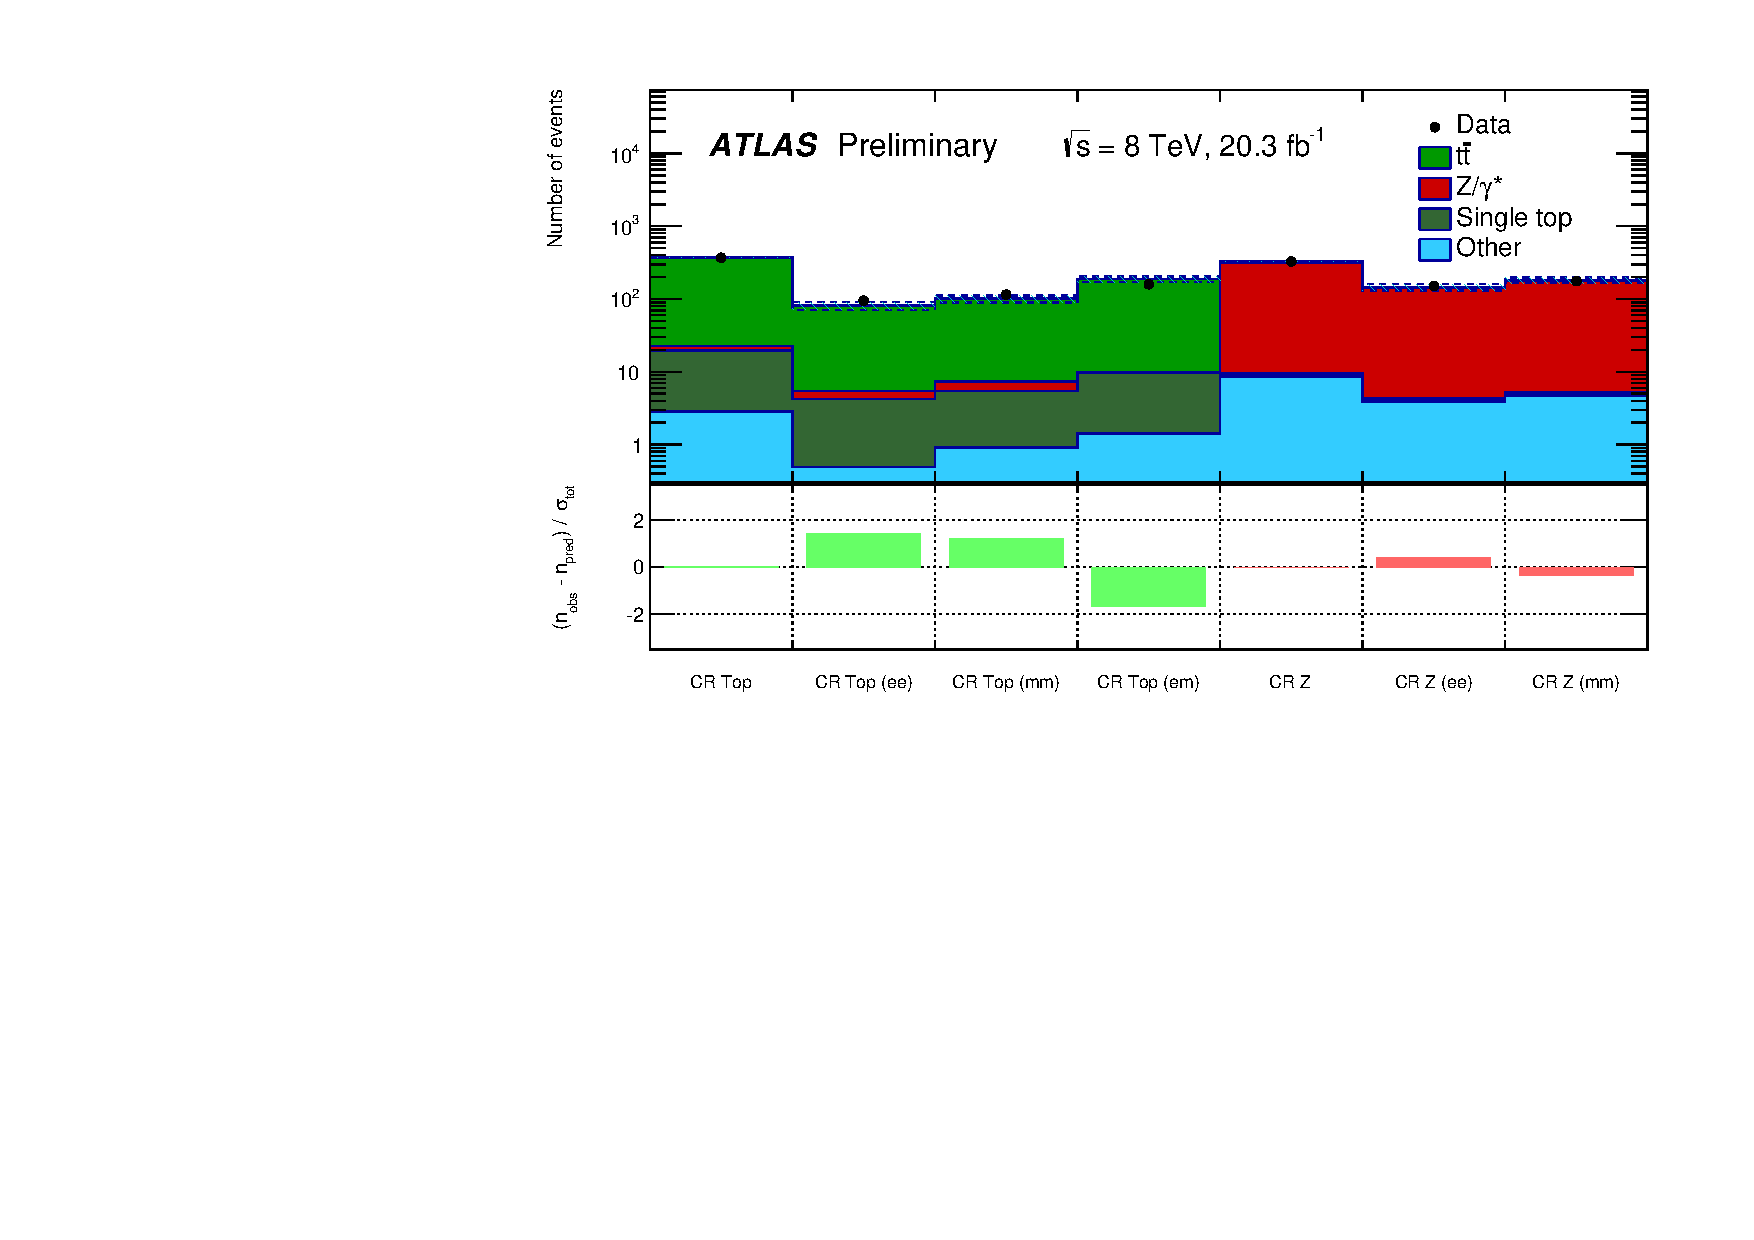
\includegraphics[width=\textwidth]{figures/blstop/histpull_CR_detailed.pdf}
  \begin{itemize}
    \item \TTBAR\ and \ZGAMMA\ normalizations were constrained using a fit to
      the observed data in the control regions
    \item Systematics included as Gaussian nuisance parameters
  \end{itemize}
\end{frame}


% ------------------------------------------------------------------------------
\begin{frame}
  \frametitle{Background estimate: validation regions}
  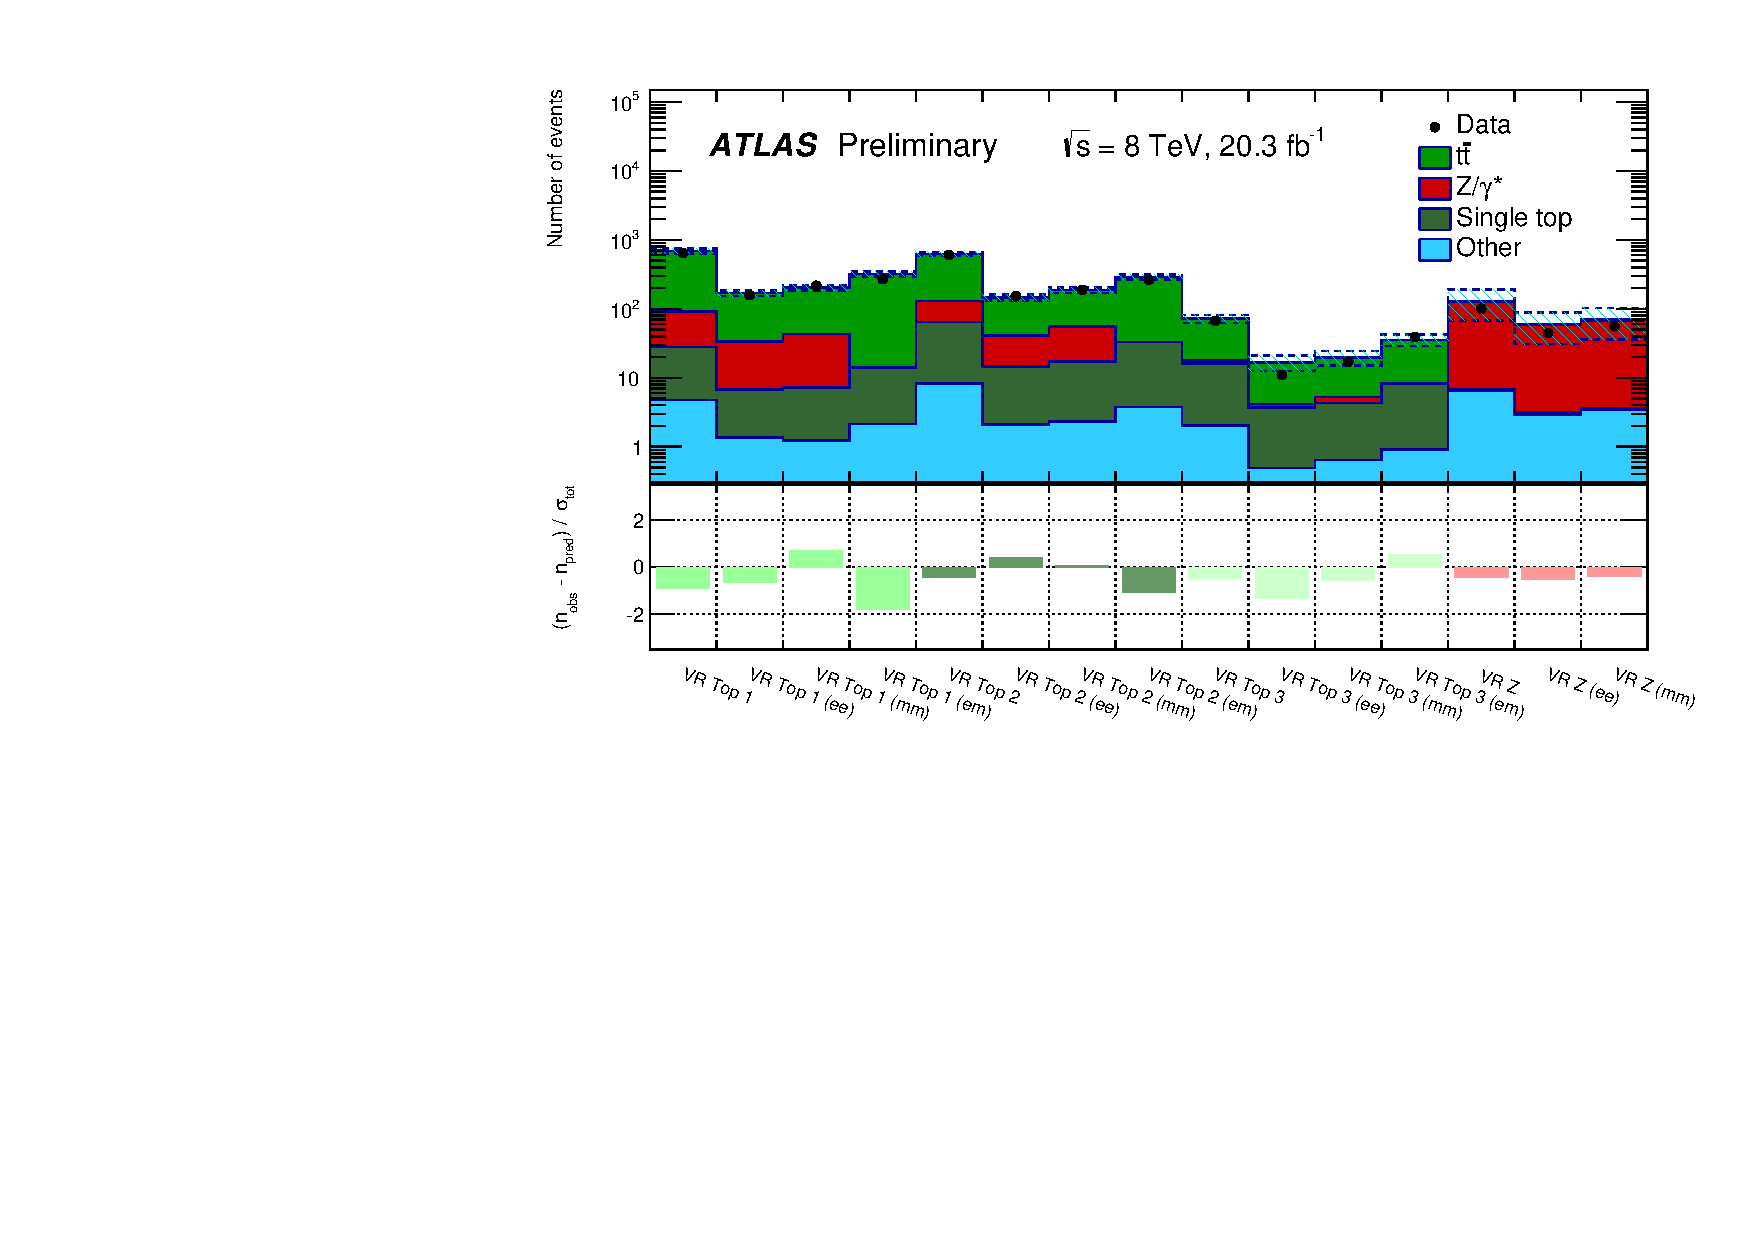
\includegraphics[width=\textwidth]{figures/blstop/histpull_VR_detailed.pdf}
  \begin{itemize}
    \item Extrapolate the fit results from the control region to the validation
      regions
    \item Overall good agreement in the validation regions
  \end{itemize}
\end{frame}


% ------------------------------------------------------------------------------
\begin{frame}
  \frametitle{Z validation region}
  %%
  \begin{columns}
    \column{0.45\textwidth}
    \begin{block}{\HT}
      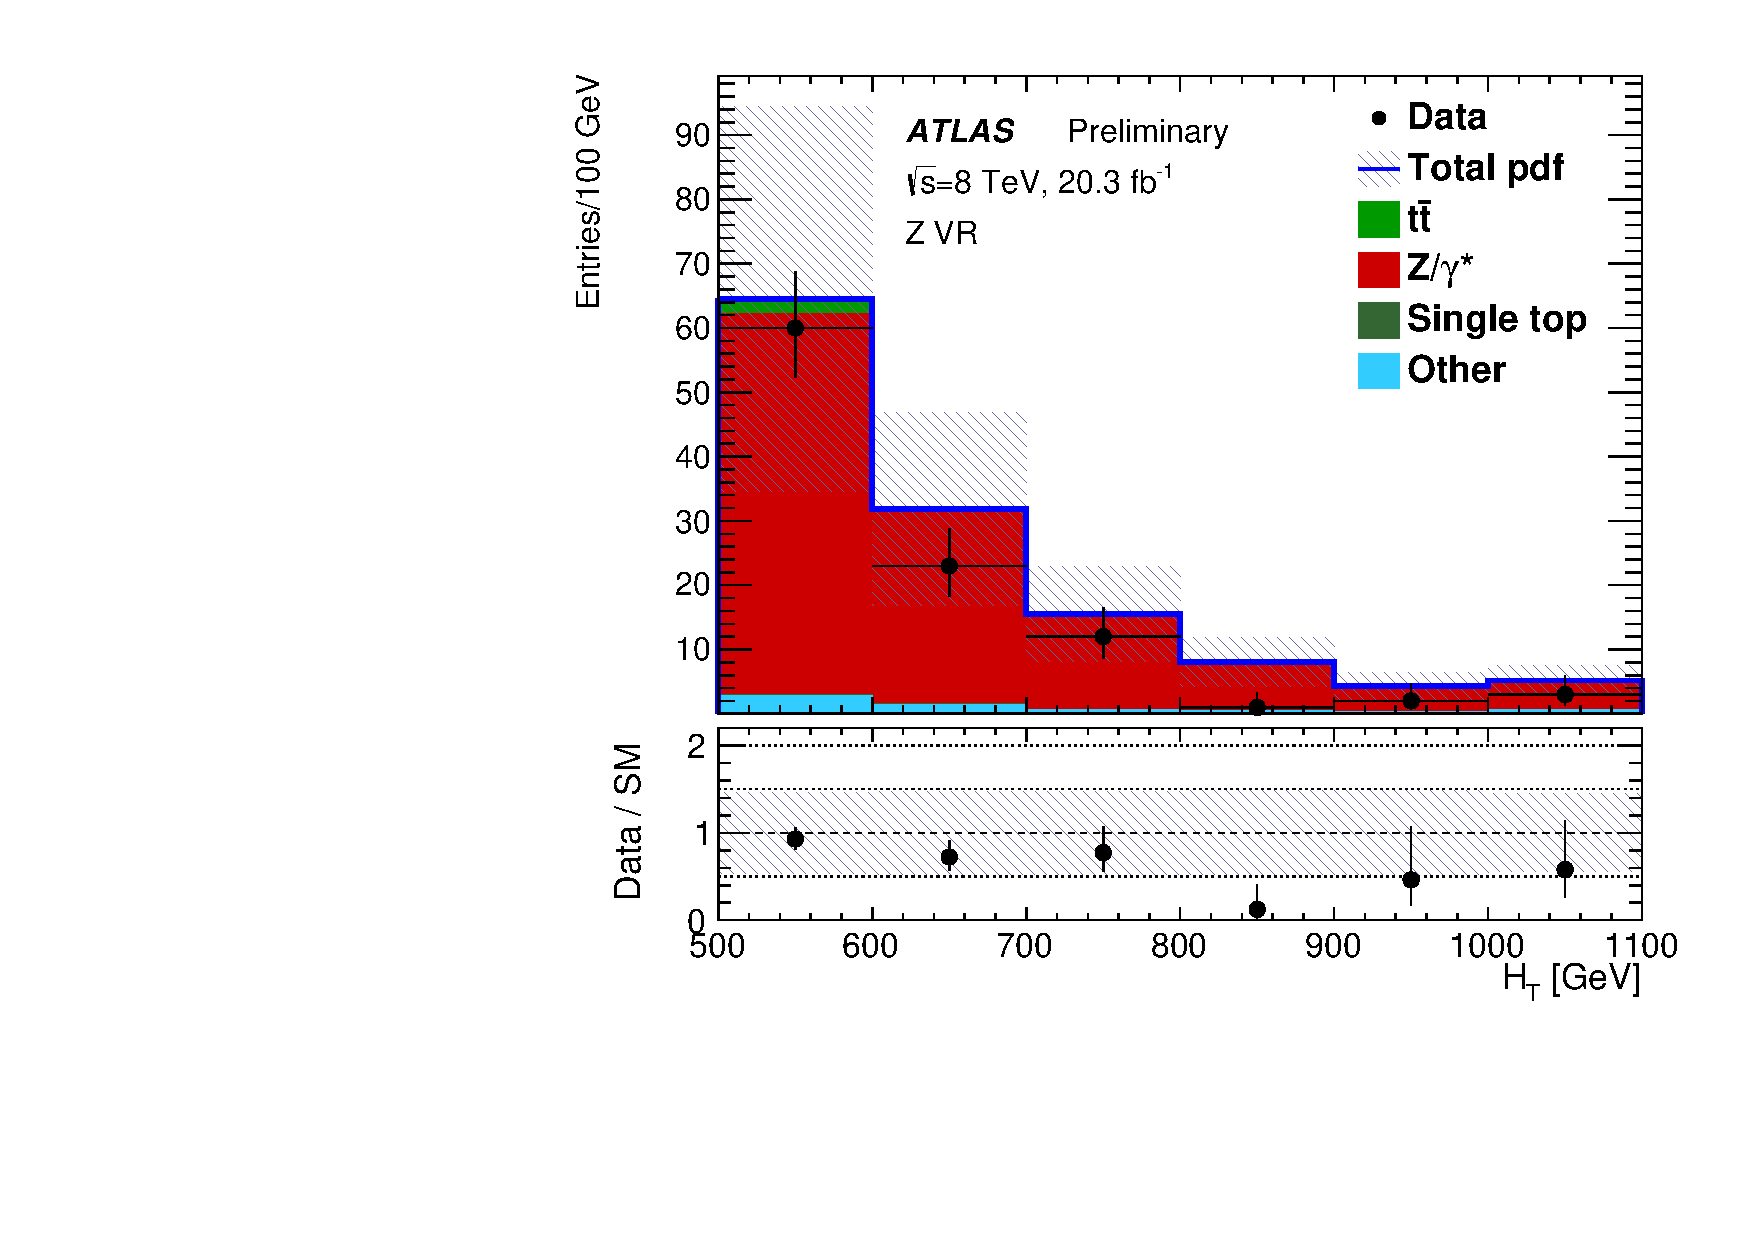
\includegraphics[width=\textwidth]{figures/blstop/vr_Z_ht_signal.pdf}
    \end{block}
    \column{0.45\textwidth}
    \begin{block}{\MBL}
      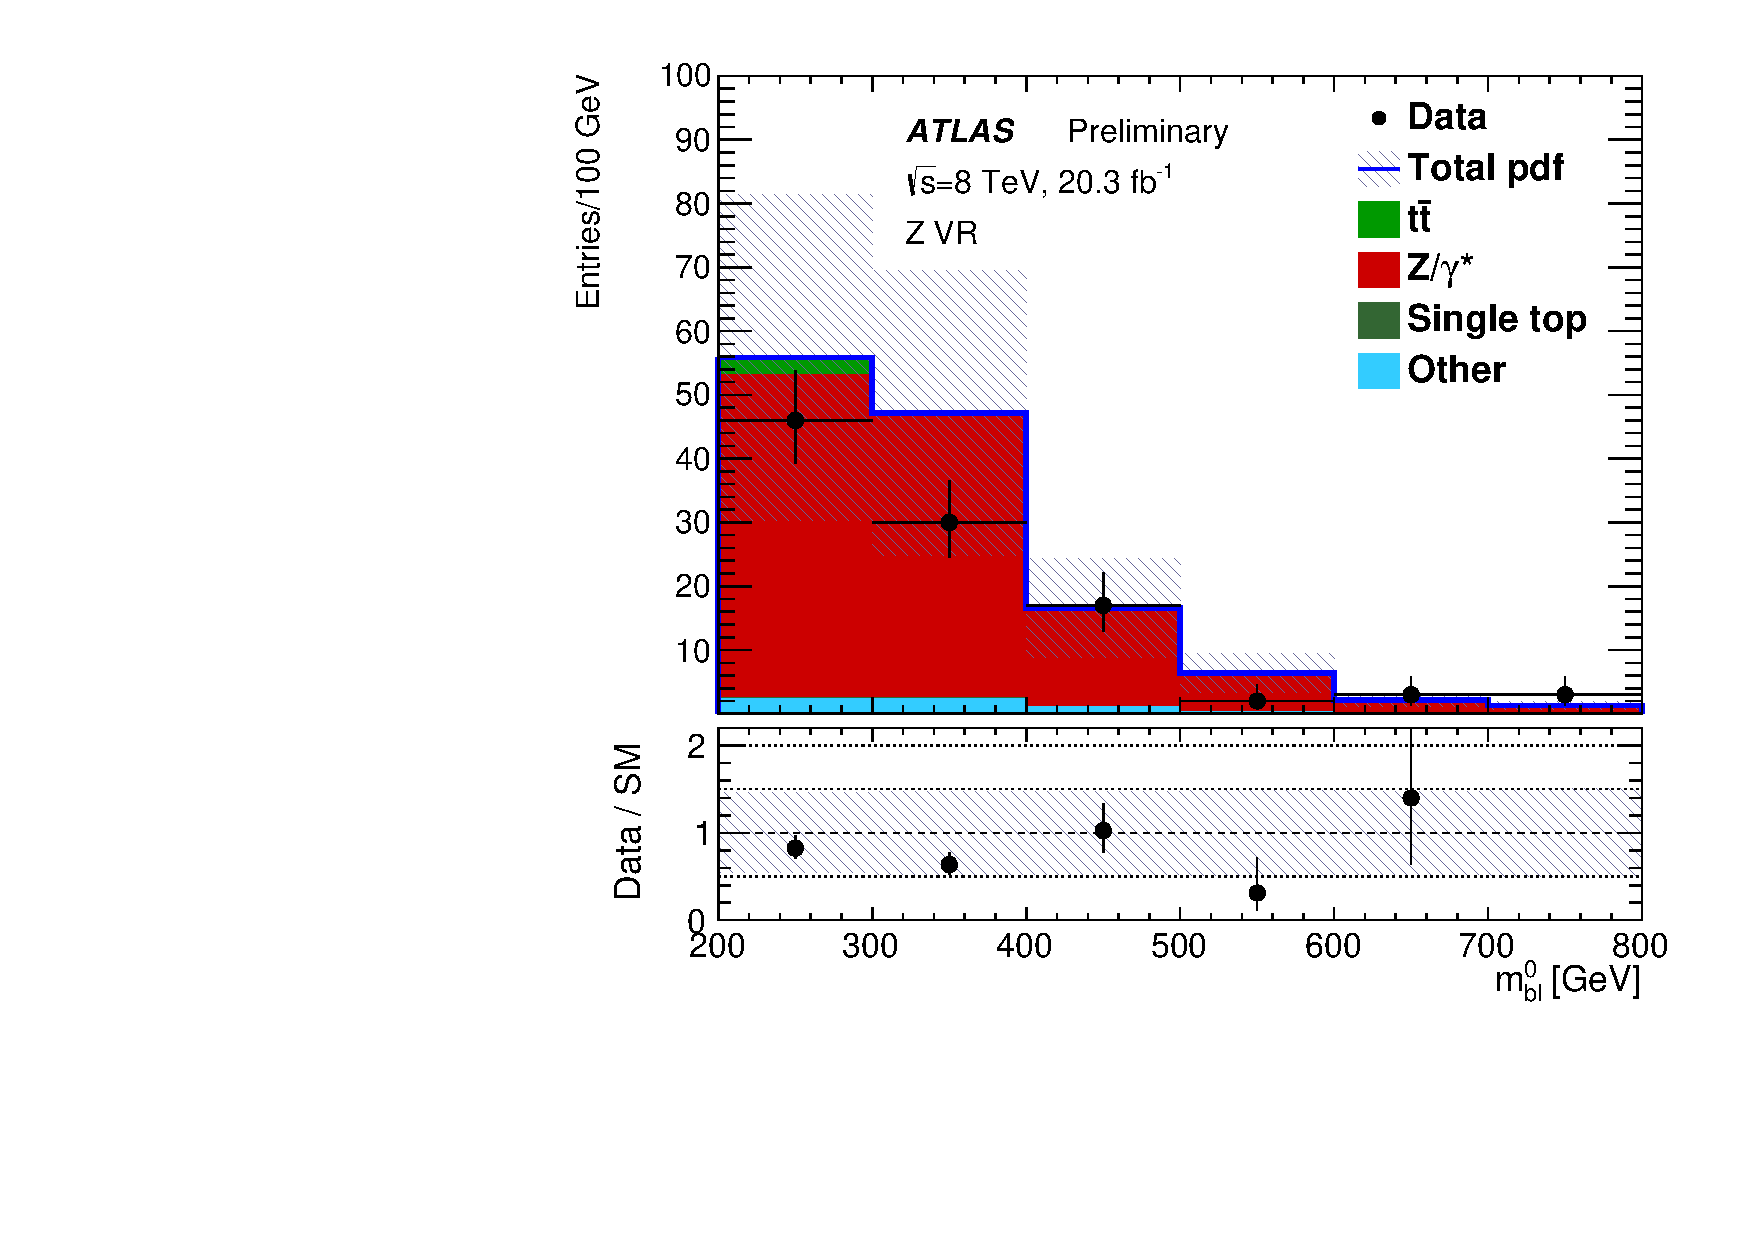
\includegraphics[width=\textwidth]{figures/blstop/vr_Z_mbl_0.pdf}
    \end{block}
  \end{columns}
  %%
  \begin{itemize}
    \item \ZGAMMA\ background is overpredicted at high \HT
    \item For this reason, an additional 50\% systematic uncertainty was taken
      on the \ZGAMMA\ background in regions with high \HT
  \end{itemize}
\end{frame}


% ==============================================================================
\subsection{Results}

% ------------------------------------------------------------------------------
\begin{frame}
  \frametitle{Results - SR 400}
  %%
  \begin{center}
    \resizebox{\textwidth}{!}{
      \begin{tikzpicture}
        \node[
          anchor=south west,
          inner sep=0
        ] (image) at (0,0) {
          \begin{tabular}{lrrrr}
            \toprule
            & SR~400                & SR~400 $ee$           & SR~400 $\mu\mu$       & SR~400 $e\mu$  \\
            \midrule
            Observed                     & $2$                   & $0$                   & $2$                   & $0$                \\
            \midrule
            Fitted bkg                   & $1.39 \pm 0.35$       & $0.36 \pm 0.15$       & $0.57 \pm 0.20$       & $0.45 \pm 0.11$    \\
            \midrule
            Fitted $t\bar{t}$            & $0.33 \pm 0.09$       & $0.07 \pm 0.08$       & $0.07 \pm 0.02$       & $0.19 \pm 0.05$    \\
            Fitted $Z/\gamma^{*}$+jets   & $0.54 \pm 0.28$       & $0.20 \pm 0.10$       & $0.35 \pm 0.18$       & $0.00 \pm 0.00$    \\
            Fitted Single Top            & $0.44 \pm 0.08$       & $0.10 \pm 0.03$       & $0.11 \pm 0.03$       & $0.23 \pm 0.05$    \\
            Fitted Other                 & $0.07 \pm 0.04$       & $0.00 \pm 0.00$       & $0.04 \pm 0.02$       & $0.03 \pm 0.03$    \\
            \midrule
            MC exp. SM                   & $1.2$                 & $0.30$                & $0.46$                & $0.43$             \\
            \midrule
            MC exp. $t\bar{t}$           & $0.30$                & $0.06$                & $0.06$                & $0.17$             \\
            MC exp. $Z/\gamma^{*}$+jets  & $0.38$                & $0.14$                & $0.24$                & $0.00$             \\
            MC exp. Single Top           & $0.44$                & $0.10$                & $0.11$                & $0.23$             \\
            MC exp. Other                & $0.07$                & $0.00$                & $0.04$                & $0.03$             \\
            \midrule
            $\sigma_\mathrm{vis}$~[fb]   & 0.23                  & 0.11                  & 0.26                  & 0.11                  \\
            Observed $N_\mathrm{non-SM}$ & 4.8                   & 2.2                   & 5.4                   & 2.3                   \\
            Expected $N_\mathrm{non-SM}$ & ${4.0}^{+2.2}_{-1.2}$ & ${3.2}^{+1.8}_{-3.2}$ & ${3.6}^{+1.9}_{-1.5}$ & ${3.3}^{+1.8}_{-3.1}$ \\
            \bottomrule
          \end{tabular}
        };
        %%
        \begin{scope}[
            x={(image.south east)}, y={(image.north west)}
          ]
          \draw[
            nice_blue,
            ultra thick,
            rounded corners
          ]
          (0.30, 0.52)
          rectangle
          (0.46, 0.92);
          %%
          \draw[
            nice_red,
            ultra thick,
            rounded corners
          ]
          (0.33, 0.00)
          rectangle
          (0.46, 0.20);
          %%
          % \MyGrid
          %%
        \end{scope}
      \end{tikzpicture}
    }
  \end{center}
\end{frame}


% ------------------------------------------------------------------------------
\begin{frame}
  \frametitle{Results - SR 600}
  %%
  \begin{center}
    \resizebox{\textwidth}{!}{
      \begin{tikzpicture}
        \node[
          anchor=south west,
          inner sep=0
        ] (image) at (0,0) {
          \begin{tabular}{lrrrr}
            \toprule
            & SR~600                & SR~600 $ee$           & SR~600 $\mu\mu$       & SR~600 $e\mu$   \\
            \midrule
            Observed                     & $1$                   & $0$                   & $1$                   & $0$              \\
            \midrule
            Fitted bkg                   & $0.55 \pm 0.15$       & $0.15 \pm 0.06$       & $0.24 \pm 0.10$       & $0.16 \pm 0.06$  \\
            \midrule
            Fitted $t\bar{t}$            & $0.10 \pm 0.02$       & $0.03 \pm 0.01$       & $0.00 \pm 0.00$       & $0.07 \pm 0.03$  \\
            Fitted $Z/\gamma^{*}$+jets   & $0.23 \pm 0.12$       & $0.08 \pm 0.05$       & $0.15 \pm 0.08$       & $0.00 \pm 0.00$  \\
            Fitted Single Top            & $0.18 \pm 0.04$       & $0.03 \pm 0.01$       & $0.05 \pm 0.02$       & $0.09 \pm 0.03$  \\
            Fitted Other                 & $0.04 \pm 0.01$       & $0.00 \pm 0.00$       & $0.04 \pm 0.02$       & $0.00 \pm 0.00$  \\
            \midrule
            MC exp. SM                   & $0.47$                & $0.12$                & $0.20$                & $0.16$           \\
            \midrule
            MC exp. $t\bar{t}$           & $0.09$                & $0.03$                & $0.00$                & $0.06$           \\
            MC exp. $Z/\gamma^{*}$+jets  & $0.16$                & $0.06$                & $0.10$                & $0.00$           \\
            MC exp. Single Top           & $0.18$                & $0.03$                & $0.05$                & $0.09$           \\
            MC exp. Other                & $0.04$                & $0.00$                & $0.04$                & $0.00$           \\
            \midrule
            $\sigma_\mathrm{vis}$~[fb]   & 0.19                  & 0.10                  & 0.20                  & 0.10 \\
            Observed $N_\mathrm{non-SM}$ & 3.9                   & 2.1                   & 4.0                   & 2.1 \\
            Expected $N_\mathrm{non-SM}$ & ${3.5}^{+1.9}_{-1.4}$ & ${2.6}^{+1.6}_{-0.6}$ & ${3.0}^{+1.7}_{-1.0}$ & ${2.7}^{+1.6}_{-0.7}$ \\
            \bottomrule
          \end{tabular}
        };
        %%
        \begin{scope}[
            x={(image.south east)}, y={(image.north west)}
          ]
          \draw[
            nice_blue,
            ultra thick,
            rounded corners
          ]
          (0.30, 0.52)
          rectangle
          (0.46, 0.92);
          %%
          \draw[
            nice_red,
            ultra thick,
            rounded corners
          ]
          (0.33, 0.00)
          rectangle
          (0.46, 0.20);
          %%
        \end{scope}
      \end{tikzpicture}
    }
  \end{center}
\end{frame}

% ------------------------------------------------------------------------------
\begin{frame}
  \frametitle{Limit setting}
  %%
  \begin{columns}
    \column{0.40\textwidth}
    \begin{itemize}
      \item Use \cls\ method to set limits
        %%
      \item Prevents exclusion if test lacks discrimination power
        %%
      % \item Test statistic: 
      %   \[
      %     q\left( \mu \right) =
      %     -2 \ln
      %     \frac{\mathcal{L} \left( \mu, \boldsymbol{\theta} \right)}
      %     {\mathcal{L}_\mathrm{max}}
      %   \]
      %   %%
      \item 
        $\cls = \frac{\clsb}{\clb}$
        %%
      \item Exclude if $\cls < 0.05$
        %%
    \end{itemize}
    %%
    \column{0.60\textwidth}
    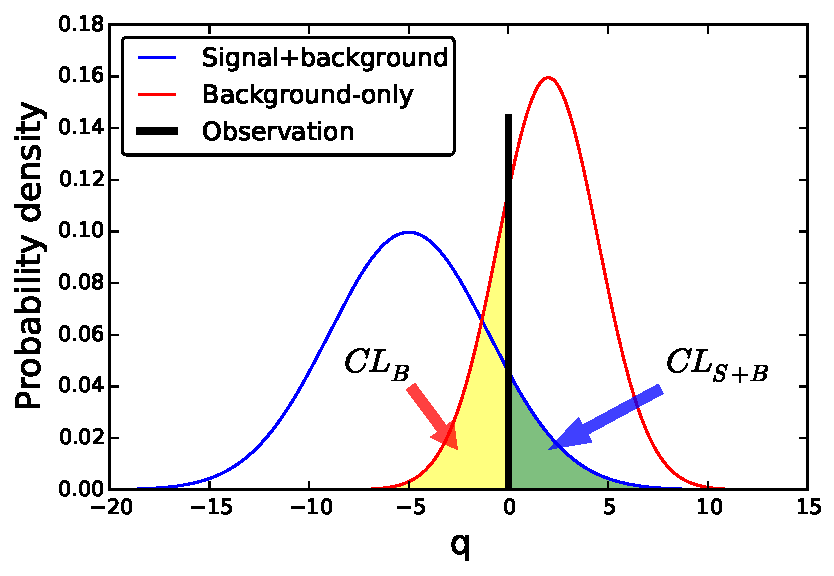
\includegraphics[width=\textwidth]{figures/cls.pdf}
    %%
  \end{columns}
\end{frame}

% ------------------------------------------------------------------------------
\begin{frame}
  \frametitle{Interpretation and limit setting}
  %%
  \begin{itemize}
    \item Stop pair branching fractions given by
      \begin{itemize}
        \item $\mathrm{Br}
          (\tilde{t}\tilde{t}^{*} \rightarrow bbee)
          =
          \mathrm{Br}(\tilde{t} \rightarrow be )^{2}$
          %%
        \item $\mathrm{Br}
          (\tilde{t}\tilde{t}^{*} \rightarrow bb\mu\mu)
          =
          \mathrm{Br}(\tilde{t} \rightarrow b\mu )^{2}$
          %%
        \item $\mathrm{Br}
          (\tilde{t}\tilde{t}^{*} \rightarrow bbe\mu)
          =
          2
          \mathrm{Br}(\tilde{t} \rightarrow be )
          \mathrm{Br}(\tilde{t} \rightarrow b\mu )$
          %%
      \end{itemize}
      %%
    % \item Signal MC generated with fixed branching fraction
    % \item Sample full branching fraction plane by applying scale factor based
    %   on flavor channel
    \item Sample range of branching fractions by applying scale factor based
      on flavor channel
    \item Perform \cls\ calculation for each mass and branching fraction
      combination to determine lower limits on stop mass
  \end{itemize}
  %%
  \begin{center}
    \includegraphics[width=\linewidth,
      clip=true,
      trim=0 8cm 0 8cm
    ]
    % {figures/blstop/branching_fractions_xe_yt.pdf}
    {figures/blstop/branching_fractions.pdf}
  \end{center}
\end{frame}


% ------------------------------------------------------------------------------
\begin{frame}
  \frametitle{Exclusion limits}
  %%
  \begin{center}
    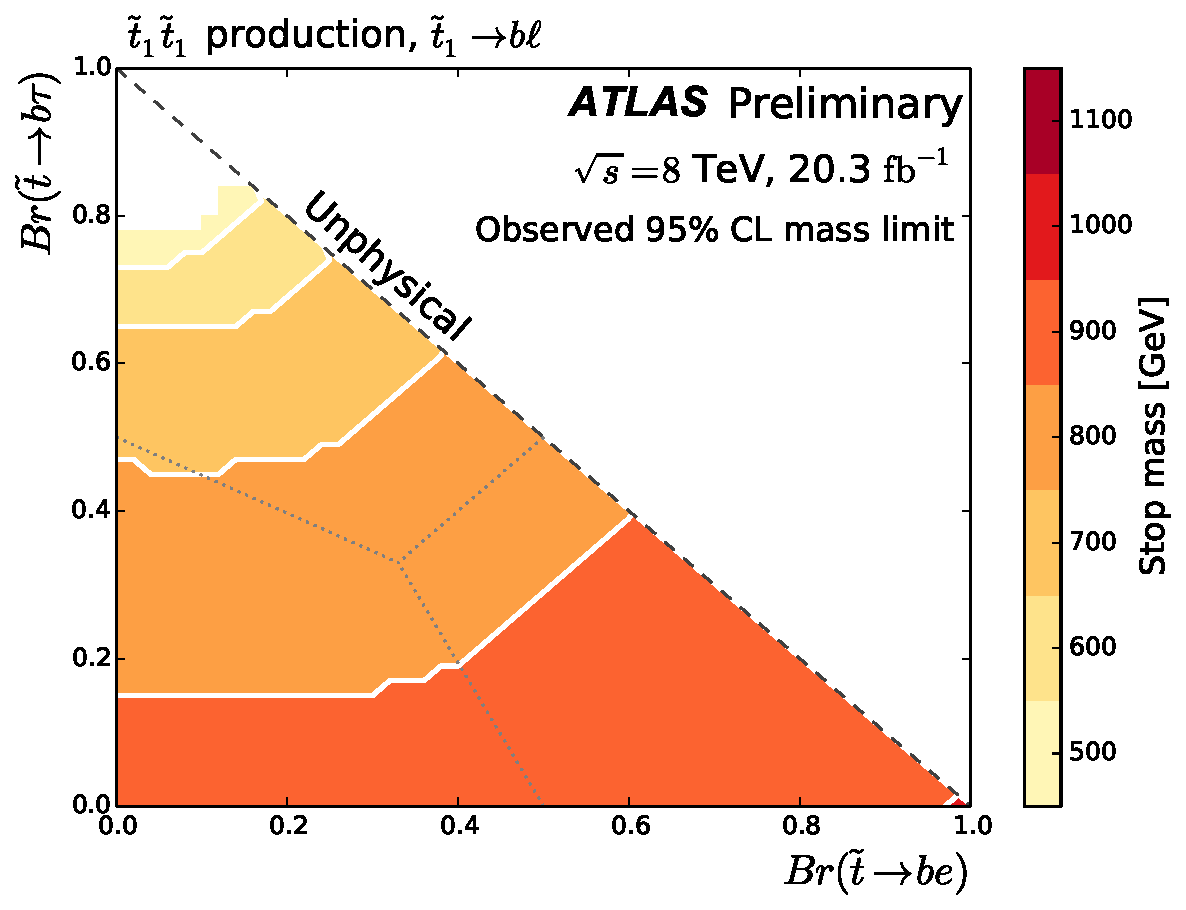
\includegraphics[width=0.9\textwidth]
    {figures/blstop/mass_limit_contours_no_extras_obs.pdf}
  \end{center}
\end{frame}


% ------------------------------------------------------------------------------
\begin{frame}
  \frametitle{Previous results}
  %%
  \begin{itemize}
    \item No direct search, but reinterpretation of leptoquark searches
  \end{itemize}
  %%
  \begin{center}
    \begin{tikzpicture}
      \node[anchor=south west, inner sep=0] (image) at (0,0) {
        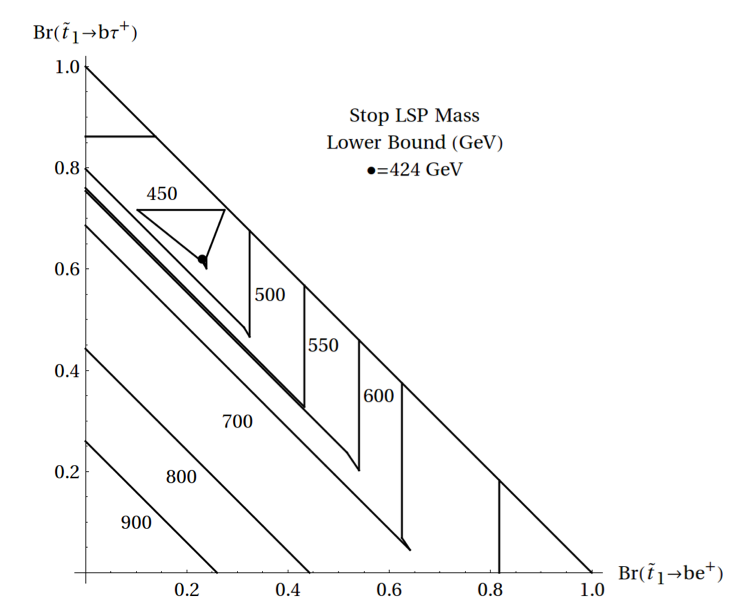
\includegraphics[width=0.6\textwidth]{figures/pheno_limit.png}
      };
      %% \begin{scope}[
      %%     x={(image.south east)},
      %%     y={(image.north west)}
      %%   ]
      %%   \node[
      %%     rectangle,
      %%     rounded corners=1ex,
      %%     fill=RoyalBlue!30!white
      %%   ]
      %%   at (0.50, 0.90) {
      %%     \scriptsize
      %%     \href{http://arxiv.org/abs/1402.5434}{arxiv:1402.5434}
      %%   };
      %%   %%
      %%   % \MyGrid
      %% \end{scope}
    \end{tikzpicture}
  \end{center}
  %%
\end{frame}


%% % ------------------------------------------------------------------------------
\begin{frame}
  \frametitle{What if we saw something?}
  %%
  \begin{itemize}
    \item \BMINUSL\ model links decay of LSP to the neutrino sector
  \end{itemize}
  %%
  \begin{center}
    \begin{tikzpicture}
      \node[
        anchor=south west,
        inner sep=0
      ] (image) at (0,0) {
        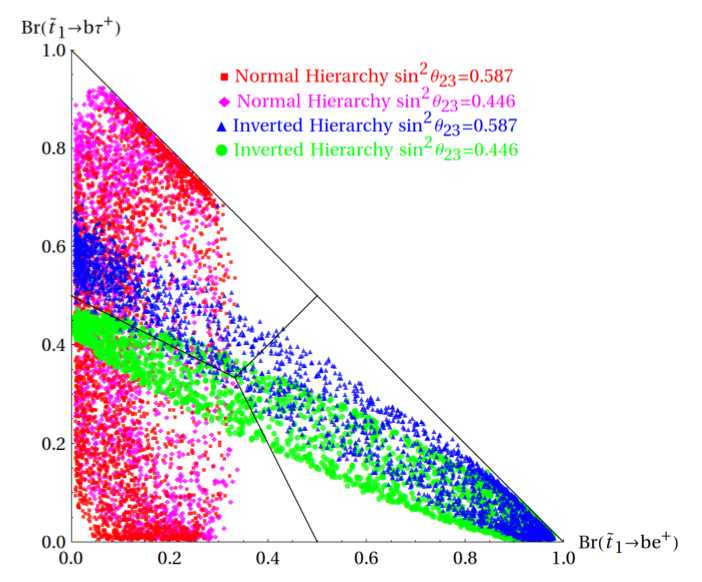
\includegraphics[width=0.55\linewidth]{figures/stop_model_scan.png}
        % 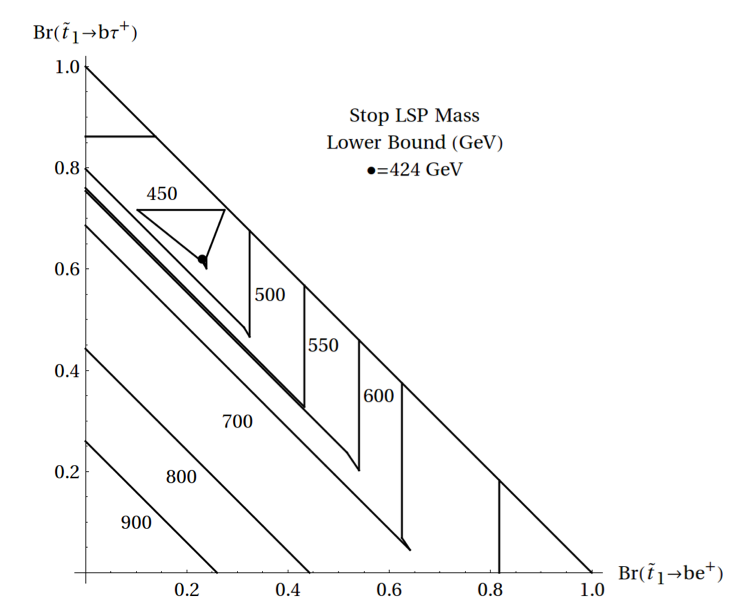
\includegraphics[width=0.60\textwidth]{figures/pheno_limit.png}
      };
      \begin{scope}[x={(image.south east)}, y={(image.north west)}]
        %% \node[rectangle,
        %%   rounded corners=1ex,
        %%   fill=RoyalBlue!30!white
        %% ] at (0.50, 0.95) {
        %%   \scriptsize
        %%   \href{http://arxiv.org/abs/1402.5434}{arxiv:1402.5434}
        %% };
        \node[
          rectangle,
          rounded corners=1ex,
          fill=RoyalBlue!80!white,
          text=white
        ] at (0.94, 0.15) {
          \small
          Mostly $bb\,ee$
        };
        \node[
          rectangle,
          rounded corners=1ex,
          fill=RoyalBlue!80!white,
          text=white
        ]
        at (-0.10, 0.15) {
          \small
          Mostly $bb\,\mu\mu$
        };
        \node[
          rectangle,
          rounded corners=1ex,
          fill=RoyalBlue!80!white,
          text=white
        ]
        at (0.37, 0.95) {
          \small
          Mostly $bb\,\tau\tau$
        };
        %% \node[
        %%   rectangle,
        %%   rounded corners=1ex,
        %%   fill=ForestGreen!80!white,
        %%   text=white
        %% ]
        % at (0.85, 0.5) {
        %   \footnotesize
        %   \begin{tabular}{c}
        %     Branching ratios of \\
        %     $\tilde{t}\rightarrow b\ell$ related to \\
        %     neutrino hierarchy
        %   \end{tabular}
        % };
        %%
        \node[
          anchor=south east,
          inner sep=0
        ] (image) at (0.02,0.27) {
          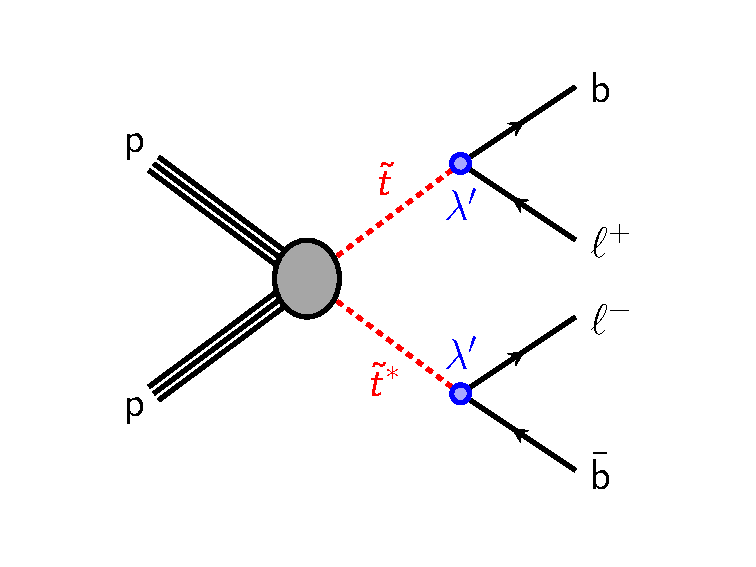
\includegraphics[width=0.4\linewidth]{figures/b_minus_l_stop_stop.pdf}
        };
        %%
        % \MyGrid
        %%
      \end{scope}
      %%
    \end{tikzpicture}
    % \end{columns}
  \end{center}
  %%
\end{frame}

% ==============================================================================
\section{Conclusions}

% ------------------------------------------------------------------------------
\begin{frame}
  \frametitle{Conclusions}
  %%
  \begin{itemize}
    \item Searched for stop pair production
      \begin{itemize}
        \item Stop decays via $R$-Parity violating coupling to $b$-quark and lepton
        \item Focus on final state with light leptons
      \end{itemize}
    \item First analysis targeting this model!
    \item No sign of SUSY yet \Simley{-0.5}
    \item Set limits between 500~\GeV\ and 1~\TeV\ depending on stop branching
      fraction
  \end{itemize}
  %%
  \vspace{1ex}
  %%
  \begin{columns}
    \column{0.5\linewidth}
    \begin{center}
      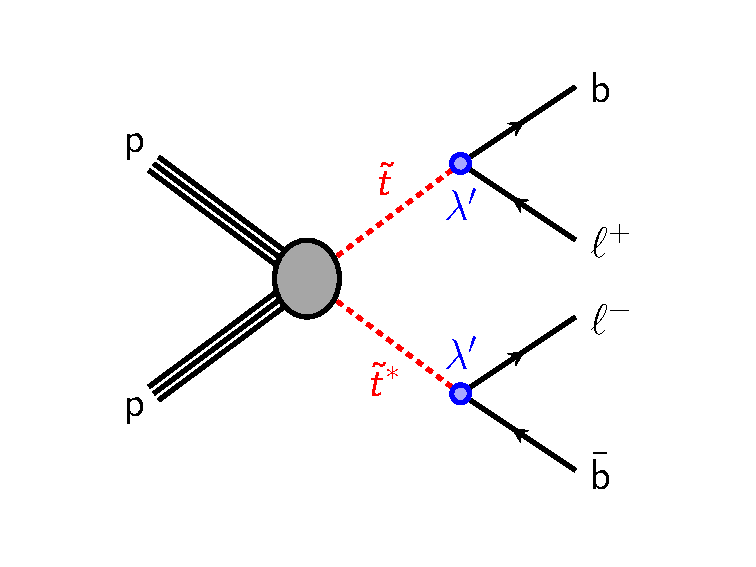
\includegraphics[width=0.9\textwidth]
      {figures/b_minus_l_stop_stop.pdf}
    \end{center}
    \column{0.5\linewidth}
    \begin{center}
      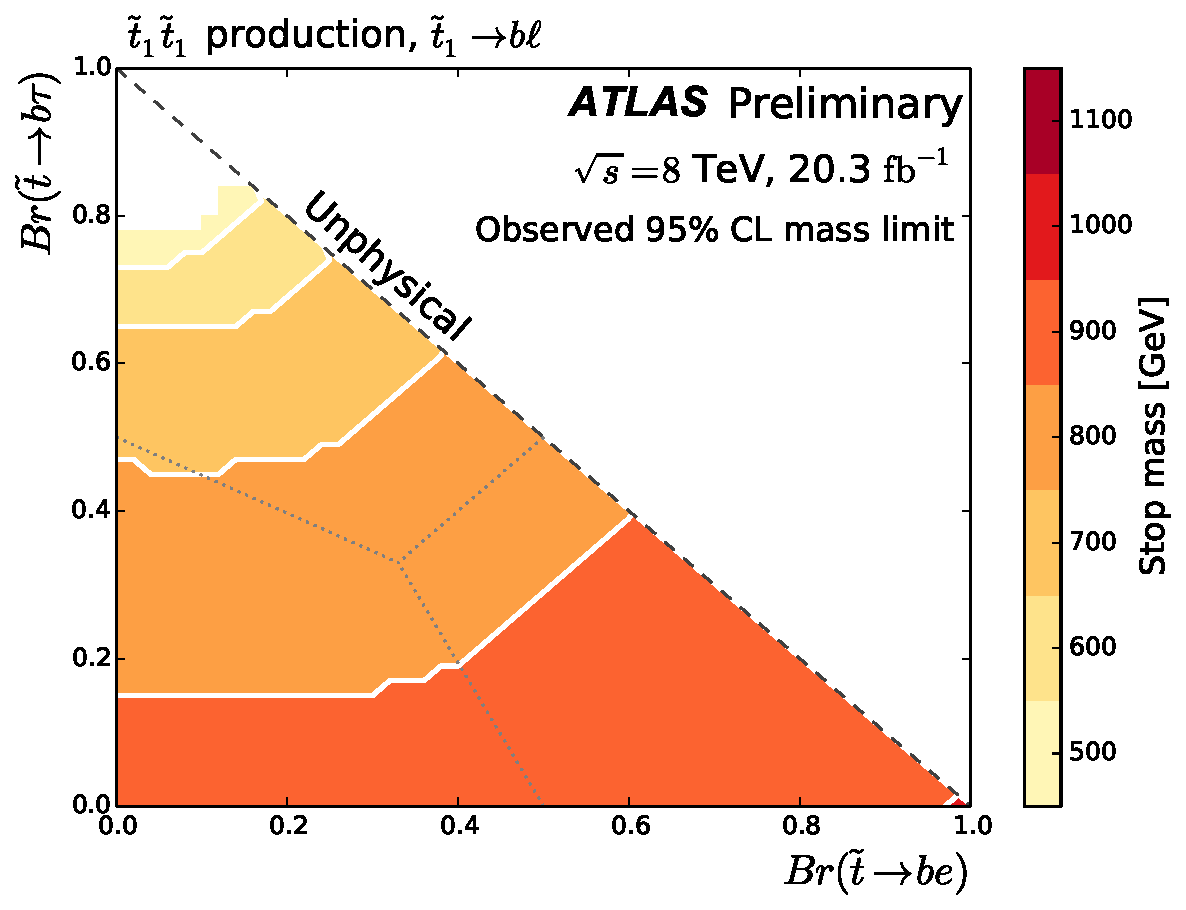
\includegraphics[width=0.9\textwidth]
      {figures/blstop/mass_limit_contours_no_extras_obs.pdf}
    \end{center}
  \end{columns}
\end{frame}

% ------------------------------------------------------------------------------
\beginbackup

% ------------------------------------------------------------------------------
\begin{frame}
  \begin{center}
    {\Huge \color{nice_blue} Backup}
  \end{center}
\end{frame}

% ------------------------------------------------------------------------------
\begin{frame}
  \frametitle{Object selection}
  %%
  \begin{columns}
    \column{0.4\textwidth}
    \begin{block}{Baseline objects}
      \vspace{1ex}
      \resizebox{\textwidth}{!}{
        \begin{tabular}{c|ccc}
          \toprule
          Variable                        & Electrons & Muons   & Jets          \\
          \toprule
          ID                              & Medium++  & Loose   & AntiKt4LCTopo \\
          $p_{\mathrm{T}}$ [GeV]          & $> 40$    & $> 40$  & $> 40$        \\
          $|\eta|$                        & $< 2.47$  & $< 2.4$ & $< 4.5$       \\
          % $\left| \frac{d_{0}}{\sigma(d_{0})} \right|$ & $< 3$     & $< 3$   & -             \\
          % $\left| \nicefrac{d_{0}}{\sigma(d_{0})} \right|$ & $< 3$     & $< 3$   & -             \\
          \DZEROSIG                       & $< 3$     & $< 3$   & -             \\
          $z_{0}\text{sin}(\theta)$ [mm]  & $< 0.4$   & $< 1$   & -             \\
          \bottomrule
        \end{tabular}
      }
    \end{block}
    \begin{block}{Overlap removal}
      \vspace{1ex}
      \resizebox{\textwidth}{!}{
        \begin{tabular}{lcl}
          \toprule
          Objects & Cut & Remove \\
          \midrule
          $ee$      & $\Delta R \le$ 0.05 & Lower $E_{T}$ electron \\
          jet $e$   & $\Delta R \le$ 0.20 & Jet                    \\
          jet $e$   & $\Delta R \le$ 0.40 & Electron               \\
          jet $\mu$ & $\Delta R \le$ 0.40 & Muon                   \\
          $e\mu$    & $\Delta R \le$ 0.01 & Electron and muon      \\
          $\mu\mu$  & $\Delta R \le$ 0.05 & Both muons             \\
          %% \midrule
          %% SF OS     & \multirow{2}{*}{$m_{\ell\ell} \le 12$ GeV} & \multirow{2}{*}{Electron and muon} \\
          %% leptons   &                                            & \\
          \bottomrule
        \end{tabular}
      }
    \end{block}
    \begin{block}{Signal objects}
      \vspace{1ex}
      \resizebox{\textwidth}{!}{
        \begin{tabular}{c|ccc}
          \toprule
          Variable & Electrons & Muons   & Jets\\
          \toprule
          $|\eta|$ & $\le 2.47$  & $\le 2.4$ & $\le 2.4$ \\
          $p_\mathrm{T}^{\mathrm{cone}30}/\min(p_\mathrm{T}, 60)$ &
            $\le 0.1$ &
            $\le 0.1$ & - \\
          B-Tag working point & - & - & 80 \% \\
          \bottomrule
        \end{tabular}
      }
    \end{block}
    %%
    \column{0.6\textwidth}
    \begin{itemize}
      % \item Much of selection based on EWK SS analysis
      \item Apply basic event cleaning
        \begin{itemize}
          \item Jet cleaning, cosmic muon veto, etc
        \end{itemize}
      \item Require at least two leptons with opposite charge and two
        b-tagged jets
        \begin{itemize}
          \item Select two leading lepton and two leading b-tagged jets if
            there are more than two of each
        \end{itemize}
      \item Two possible pairings for $bb\ell\ell$ system
        \begin{center}
          \resizebox{0.80\textwidth}{!}{%
            \begin{tikzpicture}
              \node[rectangle, text=black] (sel1) at (-5.0,+0.5) {Selection 1:};
              \node[rectangle, text=black] (sel2) at (-5.0,-0.5) {Selection 2:};

              \node[rectangle, rounded corners=1ex, fill=pairing_b_1, text=black] (b1) at (-3.25,+0.5) {$b_0$};
              \node[rectangle, rounded corners=1ex, fill=pairing_l_1, text=black] (l1) at (-2.50,+0.5) {$\ell_0$};
              \node[rectangle, rounded corners=1ex, fill=pairing_b_2, text=black] (b2) at (+1.25,+0.5) {$b_1$};
              \node[rectangle, rounded corners=1ex, fill=pairing_l_2, text=black] (l2) at (+2.00,+0.5) {$\ell_1$};
              \node[rectangle, text=black] (m11) at (-1.0,+0.5) {$\Rightarrow m_{b1\ell1} = m_{b\ell}^{0}$};
              \node[rectangle, text=black] (m22) at (+3.5,+0.5) {$\Rightarrow m_{b2\ell2} = m_{b\ell}^{1}$};

              \node[rectangle, rounded corners=1ex, fill=pairing_b_1, text=black] (b1) at (-3.25,-0.5) {$b_0$};
              \node[rectangle, rounded corners=1ex, fill=pairing_l_2, text=black] (l2) at (-2.50,-0.5) {$\ell_1$};
              \node[rectangle, rounded corners=1ex, fill=pairing_b_2, text=black] (b2) at (+1.25,-0.5) {$b_1$};
              \node[rectangle, rounded corners=1ex, fill=pairing_l_1, text=black] (l1) at (+2.00,-0.5) {$\ell_0$};
              \node[rectangle, text=black] (m12) at (-1.0,-0.5) {$\Rightarrow m_{b1\ell2} = m_{b\ell}^{0} $};
              \node[rectangle, text=black] (m21) at (+3.5,-0.5) {$\Rightarrow m_{b2\ell1} = m_{b\ell}^{1} $};
            \end{tikzpicture}
          }
        \end{center}
      \item Choose pairing with smallest difference in mass between two pairs
    \end{itemize}
    %%
  \end{columns}
\end{frame}


%% % ------------------------------------------------------------------------------
%% \begin{frame}
%%   \frametitle{Triggers}
%%   %%
%%   \begin{center}
%%     \begin{tikzpicture}
%%       %%
%%       \node
%%       [
%%         anchor=south west,
%%         inner sep=0
%%       ]
%%       (image) at (0,0)
%%       {
%%         \includegraphics[width=0.6\linewidth]
%%         {figures/EF_e24vhi_medium1_OR_EF_e60_medium1_OR_EF_mu36_tight.pdf}
%%       };
%%       %%
%%       \begin{scope}
%%         [
%%           x={(image.south east)},
%%           y={(image.north west)}
%%         ]
%%         \node
%%         [
%%           rectangle,
%%           rounded corners=1ex,
%%           fill=RoyalBlue!80!white,
%%           text=white
%%         ] at (0.95, 0.5)
%%         {
%%           \footnotesize
%%           \begin{tabular}{c}
%%             e24vhi\\
%%             e60 \\
%%             mu24i \\
%%             mu36
%%           \end{tabular}
%%         };
%%         % \MyGrid
%%       \end{scope}
%%     \end{tikzpicture}
%%   \end{center}
%%   %%
%%   \begin{itemize}
%%     \item The trigger selection depends on the flavor channel
%%       \begin{itemize}
%%         \item {\color{nice_blue} $ee$ events:} single electron
%%         \item {\color{nice_blue} $\mu\mu$ events:} single muon
%%         \item {\color{nice_blue} $e\mu$ events:} single electron or single muon
%%       \end{itemize}
%%       %%
%%     \item At least one selectd lepton within 
%%       {\color{nice_blue}$\Delta R \le 0.15$}
%%       of trigger object
%%   \end{itemize}
%% \end{frame}


% ------------------------------------------------------------------------------
\frame
{
  \frametitle{Region definitions}
  \begin{center}
    \resizebox{\textwidth}{!}{
      \begin{tabular}{l|ccccc}
        \toprule
        Region &
        $\MBL^0$ [GeV] &
        \HT [GeV] &
        \METSIG\ [$\mathrm{GeV}^{1/2}$] &
        \MBLASYM &
        Z region \\
        \midrule
        SR 400   & $\ge 400$  & $\ge 1100$ & --      & $\le 0.2$ & Veto   \\
        SR 600   & $\ge 600$  & $\ge 1100$ & --      & $\le 0.2$ & Veto   \\
        \midrule
        Top CR   & $\ge 200$  & $\le 500$  & $\ge 4$ & $\le 0.2$ & Veto   \\
        Z CR     & $\ge 200$  & $\le 500$  & $\le 4$ & $\le 0.2$ & Select \\
        \midrule
        Top VR 1 & $\ge 200$  & $\le 500$  & $\le 4$ & $\le 0.2$ & Veto   \\
        Top VR 2 & $\ge 200$  & $\le 500$  & -       & $\ge 0.2$ & Veto   \\
        Top VR 3 & $\ge 200$  & $\ge 500$  & $\ge 4$ & $\ge 0.2$ & Veto   \\
        Z VR     & $\ge 200$  & $\ge 500$  & --      & $\le 0.2$ & Select \\
        \bottomrule
      \end{tabular}
    }
  \end{center}

  \begin{columns}
    \column{0.5\textwidth}
    \begin{itemize}
      \item $Z$ region: Two same-flavor leptons
        with invariant mass $|m_{\ell\ell} - m_Z| \le 10$ GeV
      \item Signal regions optimized for stops with fairly high masses
    \end{itemize}
    %%
    \column{0.5\textwidth}
    \[
      \HT = \sum_{i=1}^{2} p_T^{\ell_i} + \sum_{j=1}^{2} p_T^{\mathrm{b~jet}_j}
    \]
    \[
      \MBLASYM = 
      \frac{\left(\MBL^0-\MBL^1\right)}{\left(\MBL^0+\MBL^1\right)}
    \]
    \[
      \METSIG = \frac{\MET}{\sqrt{\HT}}
    \]
    %%
  \end{columns}
}



% ------------------------------------------------------------------------------
\begin{frame}
  \frametitle{Signal region expectation}
  \begin{columns}
    \column{0.5\textwidth}
    \begin{table}
      \resizebox{\textwidth}{!}{
        \begin{tabular}{c|cc}
          \toprule
                                               & SR 400                & SR 600 \\
          \midrule
          $t\bar{t}$                           & $0.3$                 & $8.9 \cdot 10^{-2}$ \\
          $Z/\gamma^{*}$                       & $0.5$                 & $0.2$ \\
          Single top                           & $0.4$                 & $0.2$ \\
          Other                                & $6.9 \cdot 10^{-2}$   & $4.2 \cdot 10^{-2}$ \\
          \midrule
          Total                                & $1.3$                 & $0.5$ \\
          background                           & ($\pm$ $0.2$)         & ($\pm$ $0.1$) \\
          \midrule
          \multirow{2}{*}{\BMINUSL\ stop (500 GeV)}  & $110.3$               & $7.7$ \\
                                               & ($82.4$)              & ($14.4$)
          \vspace{1ex} \\
          \multirow{2}{*}{\BMINUSL\ stop (600 GeV)}  & $70.8$                & $34.6$ \\
                                               & ($52.9$)              & ($64.6$)
          \vspace{1ex} \\
          \multirow{2}{*}{\BMINUSL\ stop (700 GeV)}  & $33.8$                & $30.5$ \\
                                               & ($25.3$)              & ($56.8$)
          \vspace{1ex} \\
          \multirow{2}{*}{\BMINUSL\ stop (800 GeV)}  & $13.7$                & $12.9$ \\
                                               & ($10.3$)              & ($24.0$)
          \vspace{1ex} \\
          \multirow{2}{*}{\BMINUSL\ stop (900 GeV)}  & $5.5$                 & $5.2$ \\
                                               & ($4.1$)               & ($9.6$)
          \vspace{1ex} \\
          \multirow{2}{*}{\BMINUSL\ stop (1000 GeV)} & $2.1$                 & $2.0$ \\
                                               & ($1.6$)               & ($3.7$)
          \vspace{1ex} \\
          \bottomrule
        \end{tabular}
      }
    \end{table}
    \column{0.5\textwidth}
    \begin{itemize}
      \item Expected signal and background yields in the signal regions
      \item Assumed branching ratio of
        $Br(\stop \rightarrow be) = Br(\stop \rightarrow b\mu) = 0.5$
      \item Number in parentheses for each signal model is the
        {\color{nice_red}\textbf{expected ratio of signal to background}}
      \item Signal regions provide {\color{nice_blue}\textbf{good separation}}
        of signal and background
    \end{itemize}
  \end{columns}
\end{frame}


% ------------------------------------------------------------------------------
\begin{frame}
  \frametitle{Top control region}
  %%
  \begin{columns}
    \column{0.45\textwidth}
    \begin{block}{\HT}
      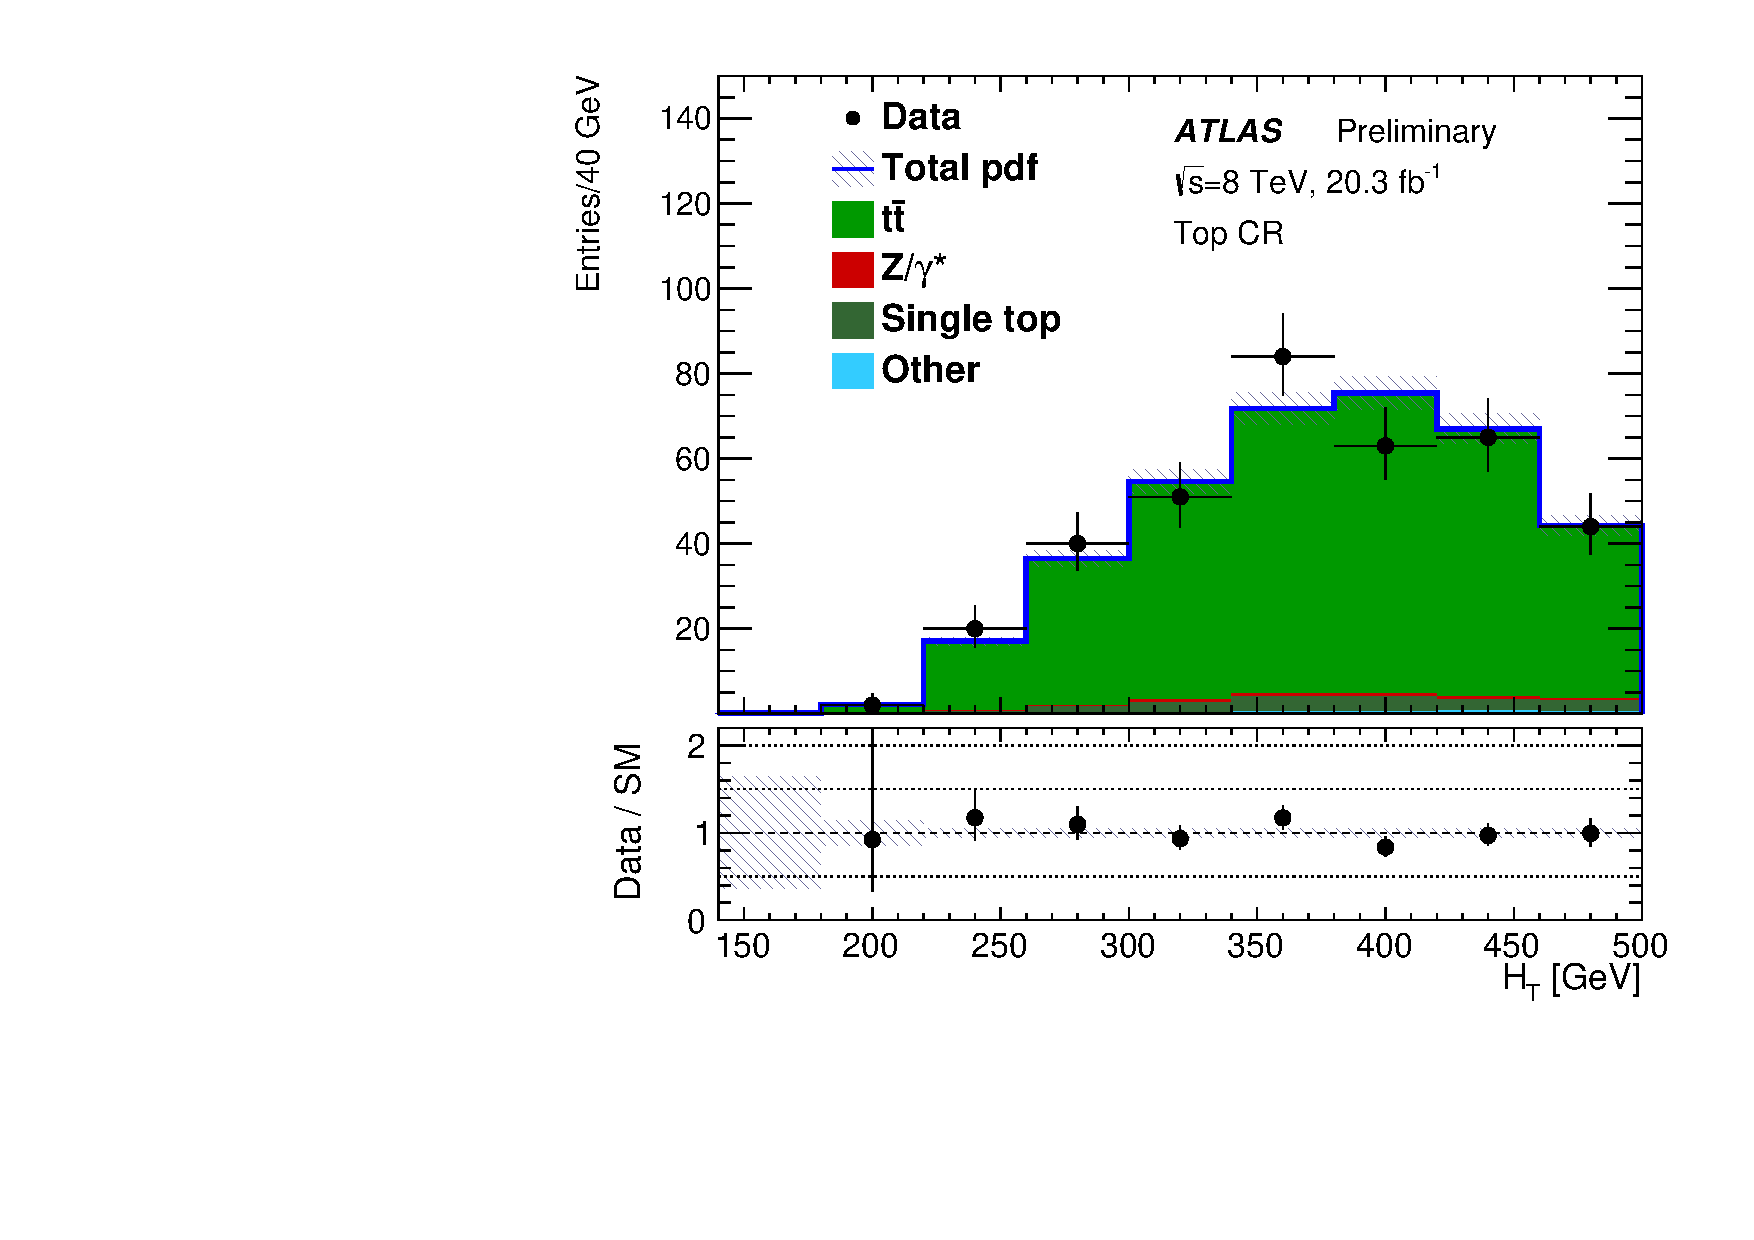
\includegraphics[width=\textwidth]{figures/blstop/cr_top_ht_signal.pdf}
    \end{block}
    \column{0.45\textwidth}
    \begin{block}{\MBL}
      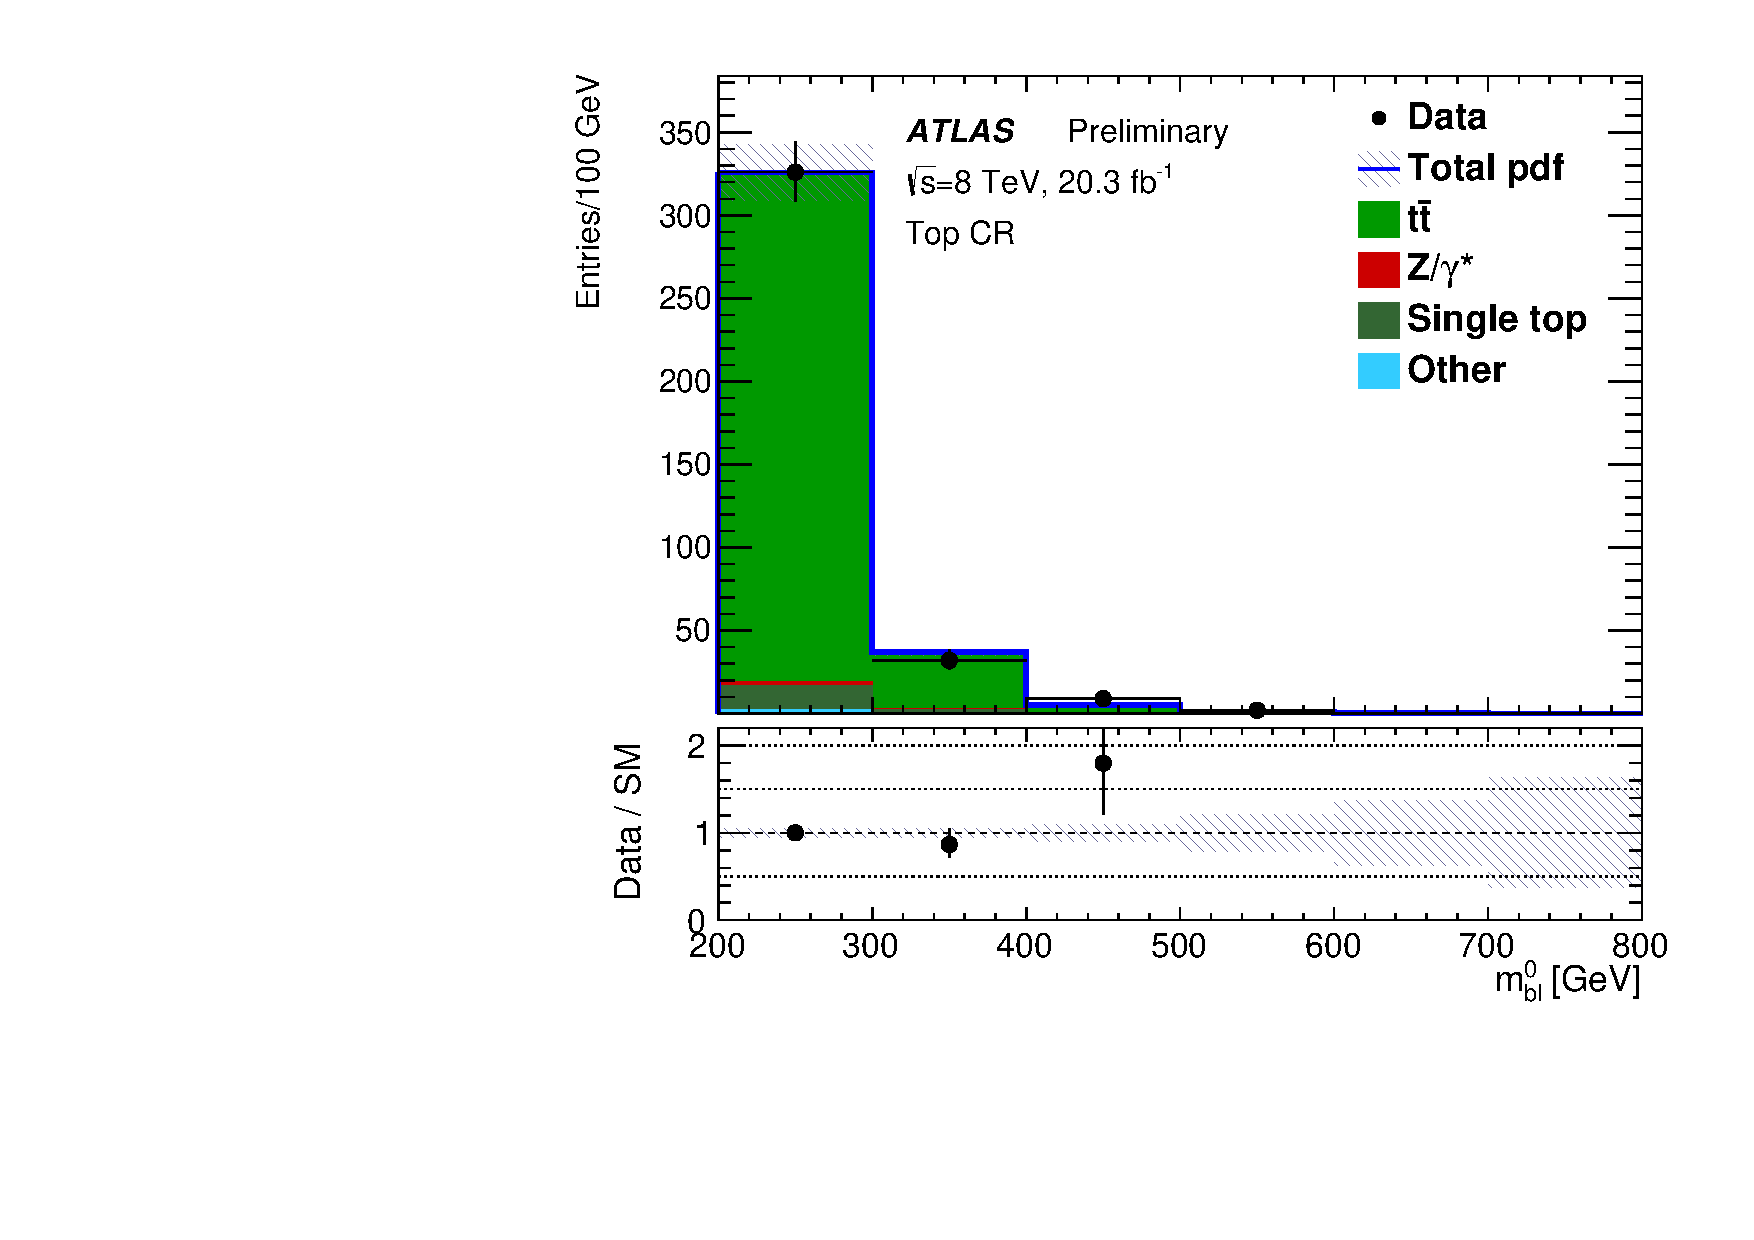
\includegraphics[width=\textwidth]{figures/blstop/cr_top_mbl_0.pdf}
    \end{block}
  \end{columns}
  %%
  \begin{itemize}
    \item Best fit normalization factor: $\mu_{\TTBAR} = 1.11 \pm 0.14$
    \item Good agreement in the top control region
    \item Top background seems to be well modeled
  \end{itemize}
\end{frame}


% ------------------------------------------------------------------------------
\begin{frame}
  \frametitle{Z control region}
  %%
  \begin{columns}
    \column{0.45\textwidth}
    \begin{block}{\HT}
      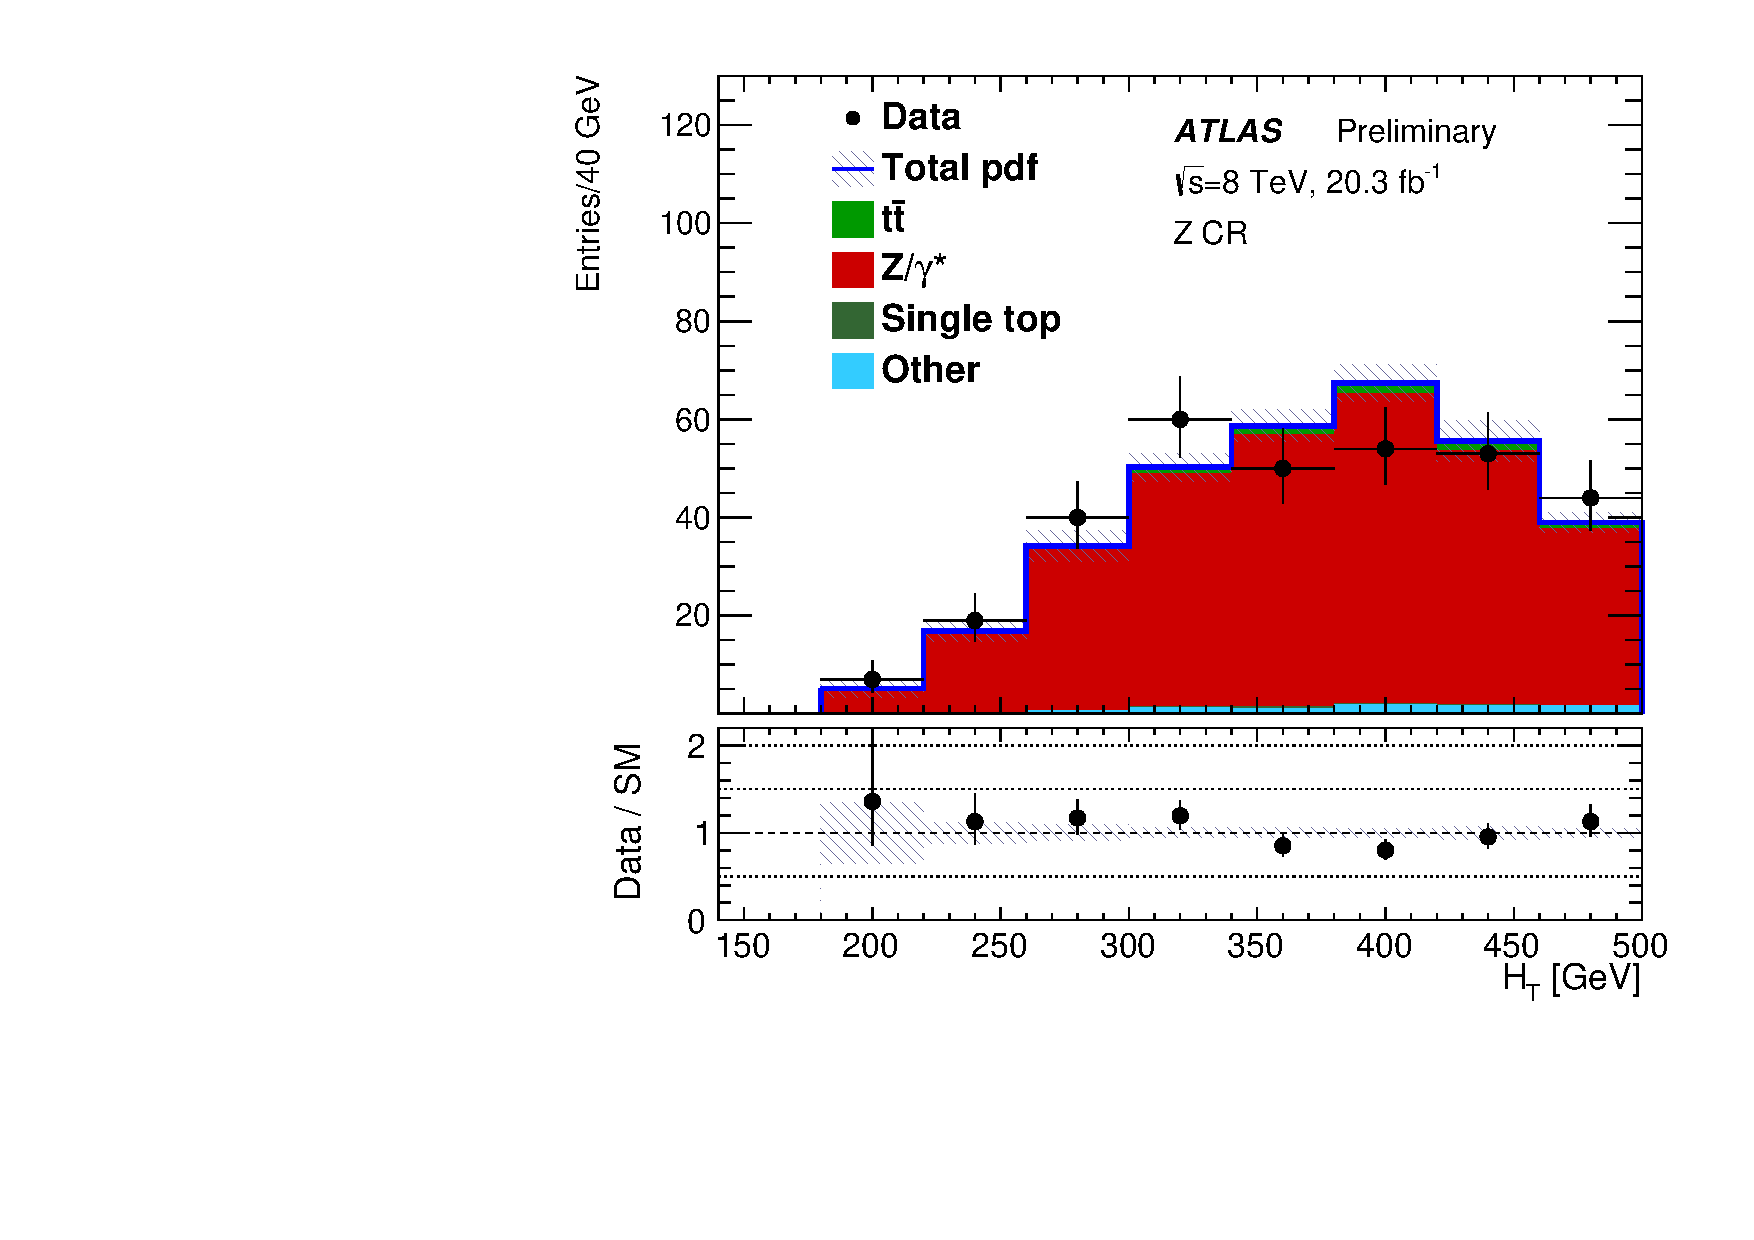
\includegraphics[width=\textwidth]{figures/blstop/cr_Z_ht_signal.pdf}
    \end{block}
    \column{0.45\textwidth}
    \begin{block}{\MBL}
      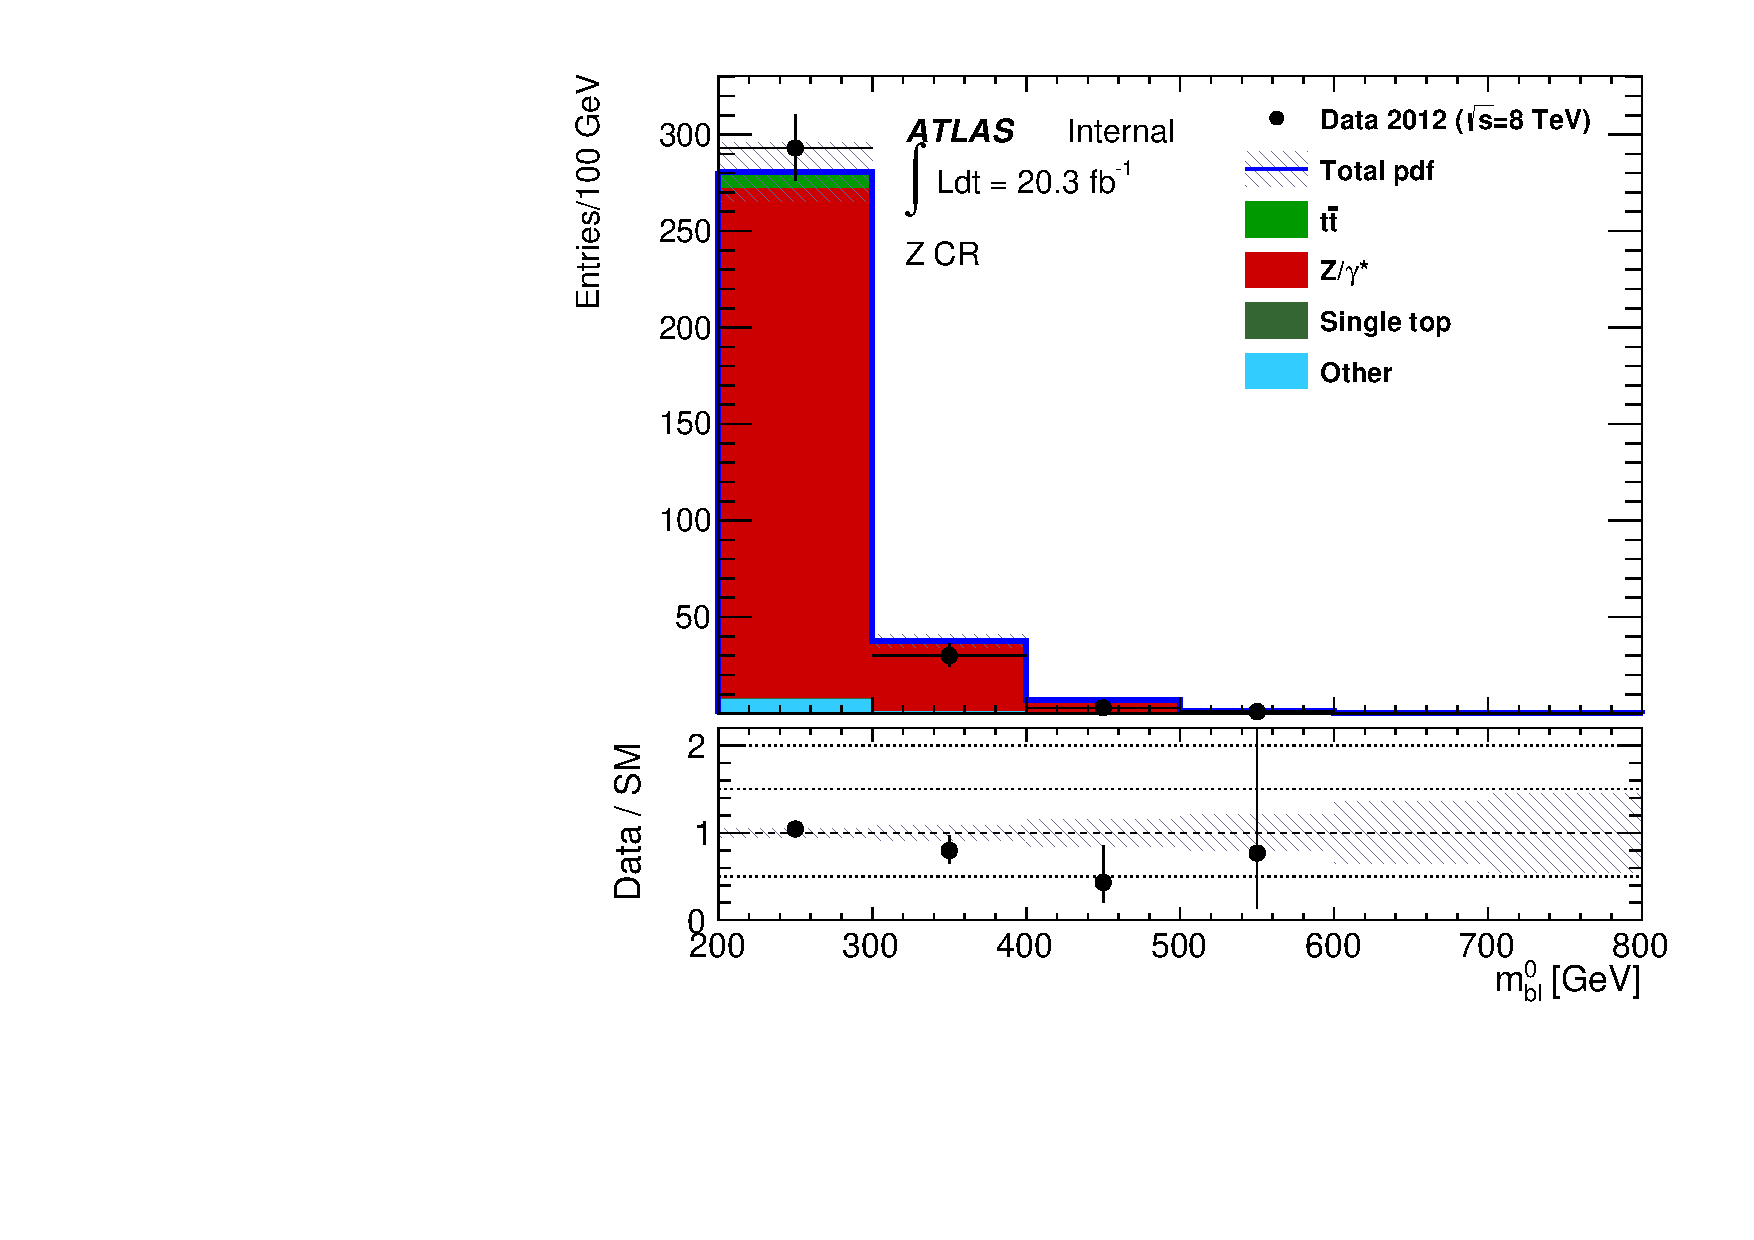
\includegraphics[width=\textwidth]{figures/cr_Z_mbl_0.pdf}
    \end{block}
  \end{columns}
  %%
  \begin{itemize}
    \item Best fit normalization factor: $\mu_{\ZGAMMA} = 1.43 \pm 0.19$
    \item Good agreement in the $Z$ control region
    \item Despite large normalization factor, the \ZGAMMA\ background seems
      well modeled in this region
  \end{itemize}
\end{frame}


% ------------------------------------------------------------------------------
\begin{frame}
  \frametitle{Top validation region 3}
  %%
  \begin{columns}
    \column{0.45\textwidth}
    \begin{block}{\HT}
      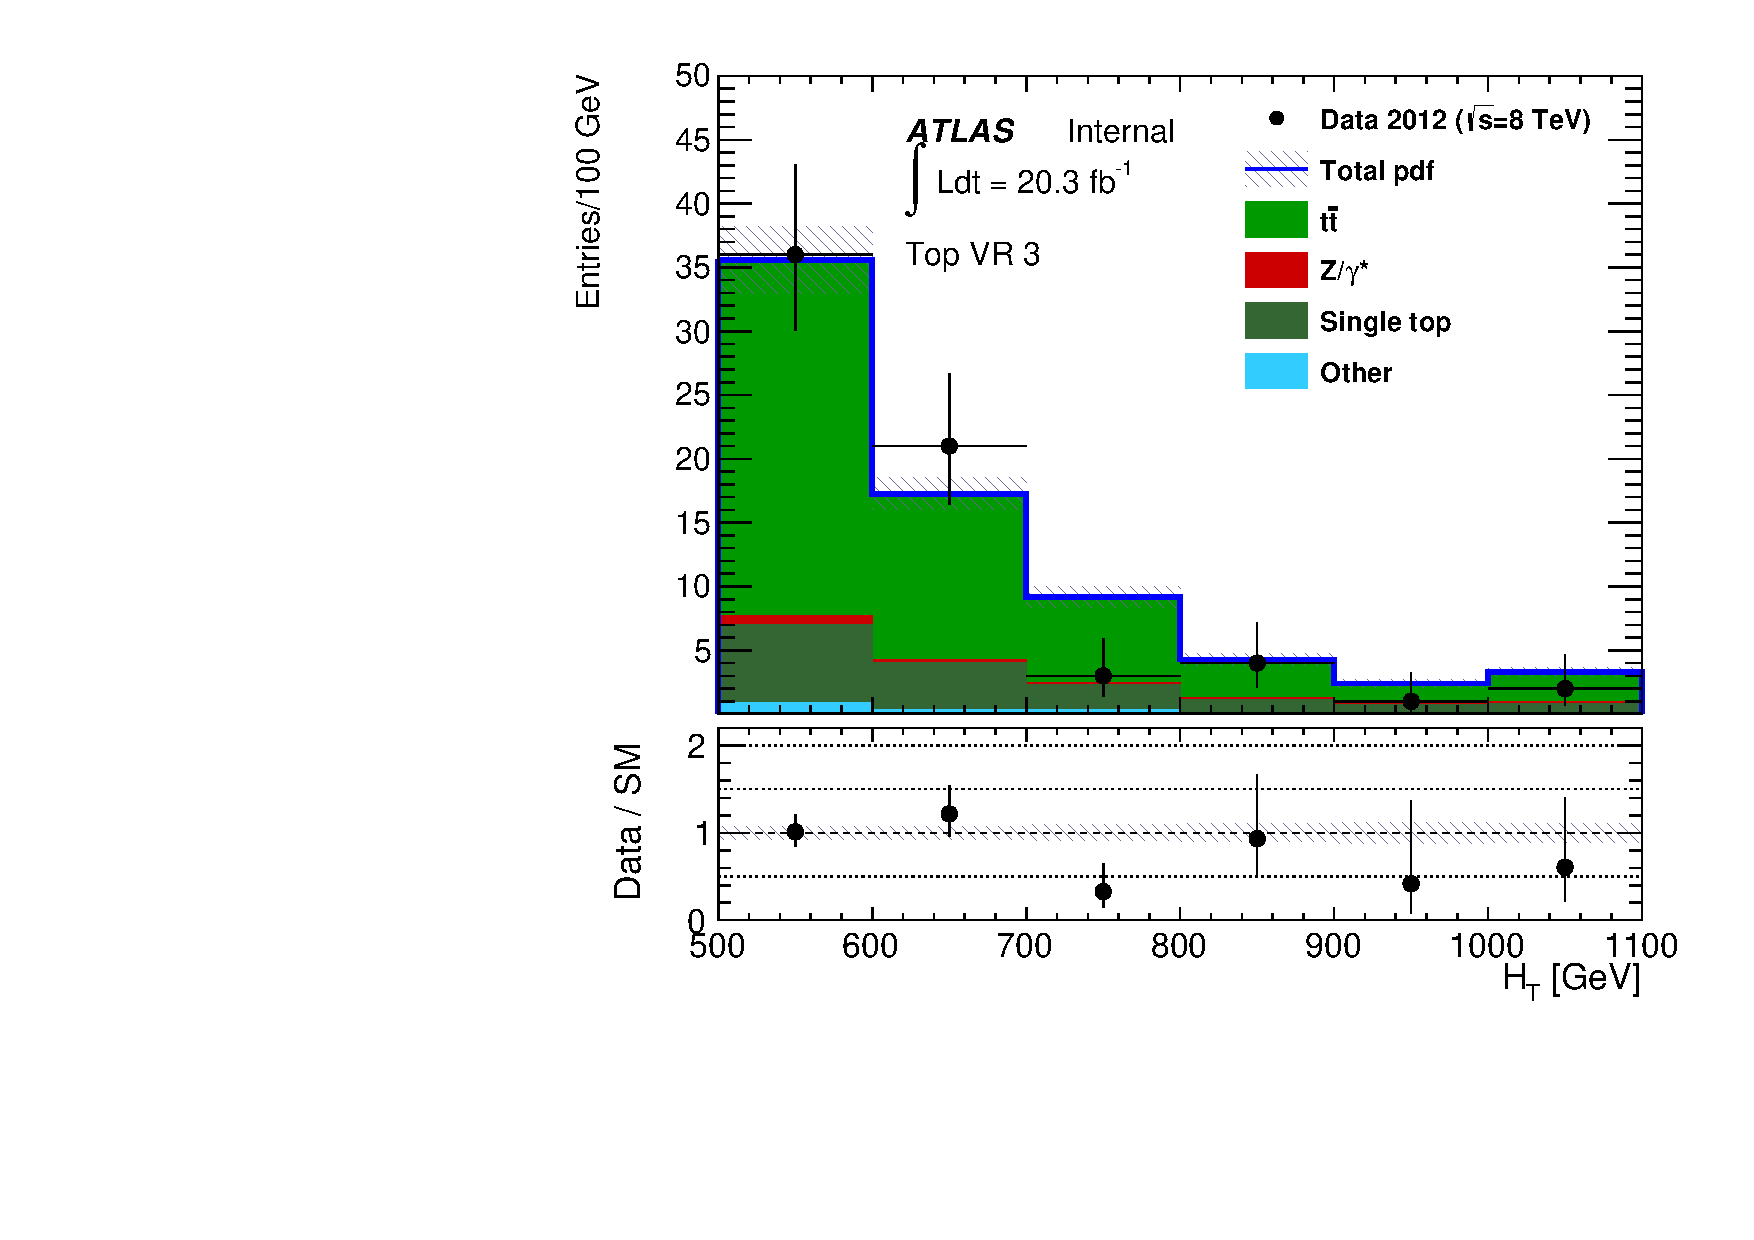
\includegraphics[width=\textwidth]{figures/vr_top_3_ht_signal.pdf}
    \end{block}
    \column{0.45\textwidth}
    \begin{block}{\MBL}
      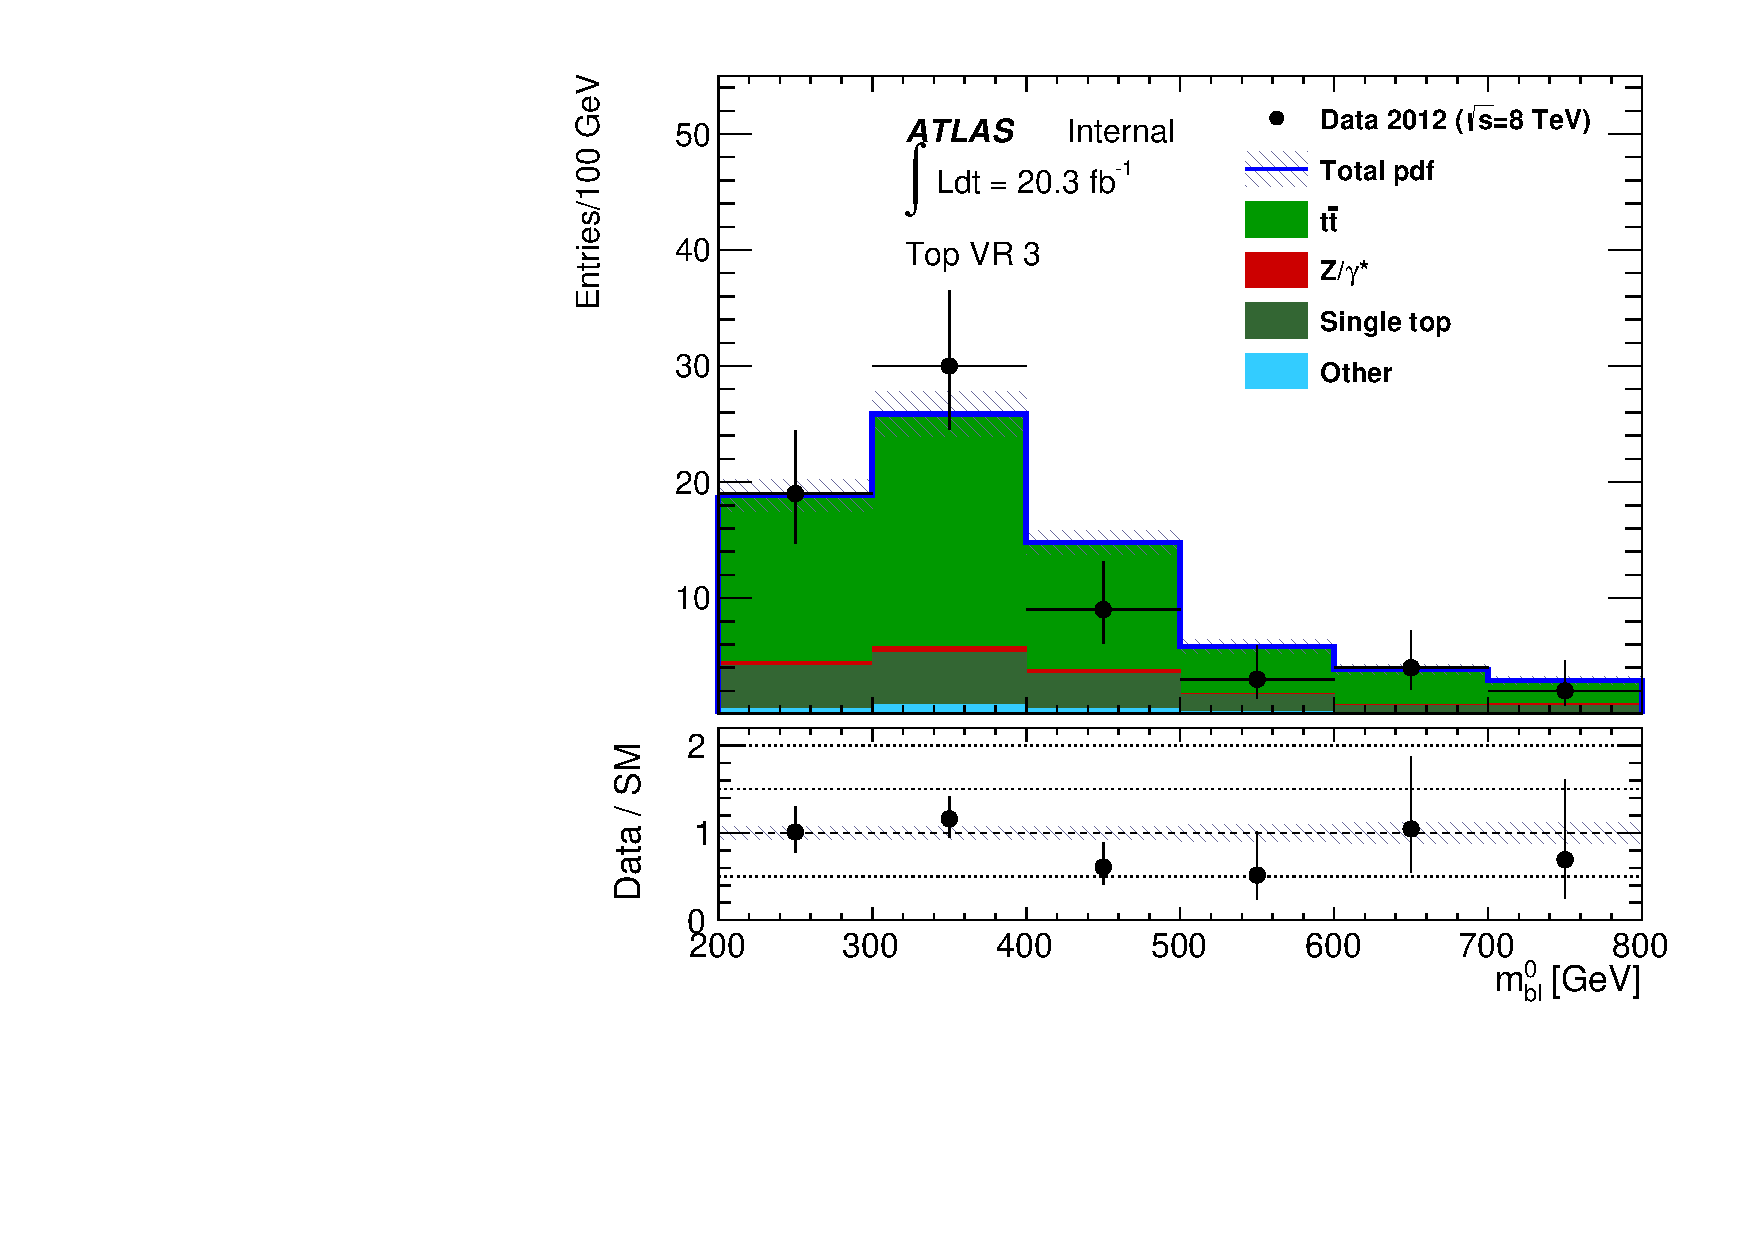
\includegraphics[width=\textwidth]{figures/vr_top_3_mbl_0.pdf}
    \end{block}
  \end{columns}
  %%
  \begin{itemize}
    \item Reasonable agreement in the top background estimate, even out to
      high \HT
    \item No need for an additional systematic uncertainty on the
      \TTBAR\ background
  \end{itemize}
\end{frame}


% ------------------------------------------------------------------------------
\begin{frame}
  \frametitle{Stop cross section}
  %%
  \begin{center}
    \includegraphics[width=0.9\textwidth]{figures/theory/xsec.pdf}
  \end{center}
\end{frame}


% ------------------------------------------------------------------------------
\begin{frame}
  \frametitle{Systematic uncertainties}
  \begin{itemize}
    \item Jet energy scale: 16 parameter JES uncertainty
    \item B-tag scale factor uncertainty
      \begin{itemize}
        \item 3 parameter uncertainty corresponding
          to b-jets, c-jets, and light flavor jets
      \end{itemize}
    \item Jet energy resolution
    \item \HT\ extrapolation
      \begin{itemize}
        \item 
          Additional 50\% uncertainty on the \ZGAMMA\ background
          in the high \HT\ region due to disagreement in Z VR 3
      \end{itemize}
    %% \item \TTBAR\ theory uncertainties
    %%   \begin{itemize}
    %%     \item Scale variations, MC generator,
    %%       Parton Shower, ISR/FSR
    %%   \end{itemize}
    %%   % ----------------------------------------------------------------------------
    %% \item Single top theory uncertainties
    %%   \begin{itemize}
    %%     \item Cross section uncertainty, MC generator, Parton Shower,
    %%       Interference with ttbar, ISR/FSR
    %%   \end{itemize}
    %%   % ----------------------------------------------------------------------------
    %% \item \ZGAMMA\ theory uncertainties
    %%   \begin{itemize}
    %%     \item Finite number of partons:
    %%   \end{itemize}
    \item Signal cross section uncertainties are taken from
      \begin{itemize}
        \item 
          {\color{nice_blue}
            \href
            {https://twiki.cern.ch/twiki/bin/view/LHCPhysics/SUSYCrossSections8TeVstopsbottom}
            {SUSYCrossSections8TeVstopsbottom}
          }
        \item See previous slide
      \end{itemize}
  \end{itemize}
\end{frame}


% ------------------------------------------------------------------------------
\begin{frame}
  \frametitle{Systematic uncertainty breakdown}
  %%
  \begin{block}{SR 400}
    \vspace{1ex}
    \resizebox{\linewidth}{!}{
      \begin{tabular}{l|cccc|c}
        \toprule
        Systematic                   & $t\bar{t}$ & $Z/\gamma^{*}$ & Single top & Other   & Total   \\
        \midrule
        Uncertainty (\%)                                                                            \\
        \midrule
        JES                          & +58/-0     & +1/-12         & +4/-4      & +5/-91  & +15/-11 \\
        $b$-tagging                  & +14/-13    & +15/-14        & +11/-10    & +12/-11 & +13/-12 \\
        JER                          & 25         & 2              & 2          & 0       & 7       \\
        Luminosity                   & -          & -              & 2          & 2       & 1       \\
        \midrule
        \HT\ extrapolation           & -          & 50             & -          & -       & 19      \\
        MC Statistical               & 25         & 4              & 10         & 50      & 13      \\
        CR Statistical               & 5          & 5              & -          & -       & 3       \\
        %% $Wt$ cross section           & -          & -              & 7          & -       & 2       \\
        %% Renormalization Scale        & 6          & -              & -          & -       & 1       \\
        %% Parton shower                & 0          & -              & -          & -       & 0       \\
        %% Multi-parton                 & -          & 0              & -          & -       & 0       \\
        %% ISR/FSR                      & 2          & -              & 0          & -       & 0       \\
        %% Factorization Scale          & 1          & -              & -          & -       & 0       \\
        %% Interference with $t\bar{t}$ & -          & -              & 0          & -       & 0       \\
        \bottomrule
      \end{tabular}
    }
  \end{block}
\end{frame}


% ------------------------------------------------------------------------------
\begin{frame}
  \frametitle{Systematic uncertainty breakdown}
  %%
  \begin{block}{SR 600}
    \vspace{1ex}
    \resizebox{\linewidth}{!}{
      \begin{tabular}{l|cccc|c}
        \toprule
        Systematic                   & $t\bar{t}$ & $Z/\gamma^{*}$ & Single top & Other   & Total   \\
        \midrule
        Uncertainty (\%)                                                                            \\
        \midrule
        JES                          & +0/-0      & +1/-4          & +6/-0      & +10/-0  & +3/-2   \\
        $b$-tagging                  & +12/-11    & +12/-11        & +12/-11    & +11/-10 & +12/-11 \\
        JER                          & 0          & 3              & 0          & 0       & 1       \\
        Luminosity                   & -          & -              & 2          & 2       & 1       \\
        \midrule
        \HT\ extrapolation           & -          & 50             & -          & -       & 20      \\
        MC Statistical               & 57         & 6              & 17         & 70      & 23      \\
        CR Statistical               & 5          & 5              & -          & -       & 3       \\
        %% $Wt$ cross section           & -          & -              & 7          & -       & 2       \\
        %% Renormalization Scale        & 0          & -              & -          & -       & 0       \\
        %% Parton shower                & 0          & -              & -          & -       & 0       \\
        %% Multi-parton                 & -          & 0              & -          & -       & 0       \\
        %% ISR/FSR                      & 0          & -              & 0          & -       & 0       \\
        %% Factorization Scale          & 16         & -              & -          & -       & 2       \\
        %% Interference with $t\bar{t}$ & -          & -              & 0          & -       & 0       \\
        \bottomrule
      \end{tabular}
    }
  \end{block}
\end{frame}

% ------------------------------------------------------------------------------
\begin{frame}
  \frametitle{Expected limits}
  %%
  \begin{center}
    \includegraphics[width=0.9\textwidth]
    {figures/blstop/mass_limit_contours_no_extras_exp.pdf}
  \end{center}
\end{frame}


% ------------------------------------------------------------------------------
\begin{frame}
  \frametitle{Exclusion limits}
  %%
  \begin{center}
    \includegraphics[width=0.9\textwidth]{figures/blstop/limit_contours.pdf}
  \end{center}
\end{frame}


%% % ------------------------------------------------------------------------------
%% \begin{frame}
%%   \frametitle{Why left-handed stops?}
%%   \UpdateFlag
%%   %%
%% \end{frame}


\backupend

\end{document}

